\documentclass[useAMS,usenatbib]{mn2e}
\usepackage{epsfig,rotate,graphicx}
\usepackage[fleqn]{amsmath}
\usepackage{subfigure}
\usepackage{lscape}
\usepackage{bm}

\newcommand{\p}{\partial}
\newcommand{\mnras}{MNRAS}
\newcommand{\apj}{ApJ}
\newcommand{\aj}{AJ}
\newcommand{\aap}{A\&A}
\newcommand{\aapr}{A\&ARv}
\newcommand{\apss}{ApSS}
\newcommand{\apjl}{ApJL}
\newcommand{\pasj}{PASJ}
\newcommand{\araa}{ARAA}
\newcommand{\dd}{\delta}
\newcommand{\adot}{\dot{a}}
\newcommand{\be}{\begin{equation}}
\newcommand{\ee}{\end{equation}}
\newcommand{\gtrsim}{\;\raisebox{-.8ex}{$\buildrel{\textstyle>}\over\sim$}\;}
\newcommand{\lesssim}{\; \raisebox{-.8ex}{$\buildrel{\textstyle<}\over\sim$}\;}
\newcommand{\anrev}{{\it ARA\&A, }}
\newcommand{\apjs}{{\it ApJS, }}
\newcommand{\icar}{{\it Icarus, }}
\newcommand{\mnr}{{\it MNRAS, }}
\newcommand{\nat}{{\it Nature, }}
\newcommand{\sci}{{\it Sci, }}
\newcommand{\ana}{{\it A\&A, }}
\newcommand{\anas}{{\it A\&AS, }}
\newcommand{\aaps}{{\it A\&AS, }}
\newcommand{\anar}{{\it A\&AR, }}
\newcommand{\prd}{{\it Phys. Rev. D }}
\newcommand{\qjl}{{\it QJRAS, }}
\newcommand{\sbar}{\bar{\sigma}}
\newcommand{\avg}[1]{\langle #1 \rangle}
\newcommand{\bu}{\bm{u}}
\newcommand{\lmax}{l_\mathrm{max}}
\newcommand{\mmax}{m_\mathrm{max}}
\newcommand{\trel}{t_\mathrm{rel}}
\newcommand{\zeus}{{\tt ZEUS-MP }}
\newcommand{\ii}{\mathrm{i}}
\newcommand{\bv}{\bm{v}}
\newcommand{\rin}{r_\mathrm{in}}
\newcommand{\rout}{r_\mathrm{out}}
\newcommand{\ciso}{c_\mathrm{iso}}
\newcommand{\tbeta}{\tilde{\beta}}
\newcommand{\teta}{\tilde{\eta}}
\newcommand{\tcool}{t_\mathrm{cool}}
\newcommand{\jlin}{j_\mathrm{lin}}
\newcommand{\jlintot}{J_\mathrm{lin}}
\newcommand{\tbg}{T_\mathrm{BG}}
\newcommand{\varA}[1]{{\operatorname{#1}}}
\DeclareMathOperator{\erf}{erf}
\DeclareMathOperator{\real}{Re}
\DeclareMathOperator{\imag}{Im}

\usepackage{array,booktabs,tabularx}
\newcolumntype{R}{>{\centering\arraybackslash}X} % right justified tabularx columns

\title[One-armed spirals]{One-armed spirals in 
  locally isothermal, radially structured self-gravitating discs}     

\author[Lin]{Min-Kai Lin$^{1}$
  \thanks{ minkailin@email.arizona.edu} \\ 
  $^1$Department of Astronomy and Steward Observatory, University of
  Arizona, 933 North Cherry Avenue, Tucson, AZ 85721, USA 
}

\begin{document}

\maketitle
\begin{abstract} 
  {\bf We describe a new mechanism that leads to the destabilisation of
  one-armed spiral or eccentric modes in astrophysical discs with 
  an imposed radial temperature gradient.  We use linear density wave
  theory 
  to show that non-axisymmetric perturbations generally do not conserve
  their angular momentum in the presence of a forced temperature
  gradient. This implies an exchange of angular momentum
  between linear perturbations and the background disc. In particular, 
  when the disturbance is a low-frequency, one-armed
  trailing spiral and the disc temperature decreases outwards, this 
  interaction is unstable and leads to the growth of the spiral mode.  
  We demonstrate this phenomenon through numerical hydrodynamic
  simulations of locally isothermal discs in 2D using the FARGO
  code and in 3D with  the ZEUS-MP and PLUTO codes.  We consider
  radially structured discs with a self-gravitating sub-portion which remains
  stable in the absence of a temperature gradient. However,
  when a temperature gradient is imposed we observe exponential growth of an one-armed  
  spiral mode (azimuthal wavenumber $m=1$) with co-rotation radius 
  outside the bulk of the spiral arm, resulting in a low-frequency  
  spiral pattern in the self-gravitating region of the disc.  The development of this one-armed 
 spiral does not require the movement of the central star, as found in previous studies. 
 Because destabilisation by the imposed temperature gradient does 
 not explicitly depend on self-gravity, we suggest this mechanism may also
 affect low-frequency one-armed oscillations in non-self-gravitating
 discs. 
}
\end{abstract}


%This might represent, for example, mass  
 % built-up in a circumstellar or protoplanetary
 % disc at the outer edge of a `dead zone', in which there
  %is inefficient magneto-hydrodynamic turbulence to enable accretion. 

\begin{keywords}
  accretion, accretion discs, hydrodynamics, instabilities, methods: numerical, protoplanetary discs 
\end{keywords}

\section{Introduction}\label{intro}
% Protoplanetary discs are expected to contain complex structures
% \citep{armitage11}, which directly impact planet formation theories.  
An exciting development in the study of circumstellar 
discs is the direct observation of large-scale, non-axisymmetric
structures within them. These
include lopsided dust distributions 
\citep{marel13,fukagawa13,casassus13,isella13,perez14,follette14} and
spiral arms 
\citep{hashimoto11,muto12,boccaletti14,grady13,christiaens14,avenhaus14}. 

% planet is popular answer for spiral structure
The attractive explanation for asymmetries in circumstellar discs is
disc-planet interaction. In particular, spiral structures  
naturally arise from the gravitational interaction between a
planet and the gaseous protoplanetary disc it is embedded in
\citep[see, e.g.][for a recent review]{baruteau13b}. Thus, the
presence of spiral arms in circumstellar discs could be signposts of 
planet formation.  

% but also natural in GI.
However, spiral arms are also associated with global gravitational 
instability (GI) of differentially rotating discs
\citep{goldreich65,laughlin96b,laughlin98,nelson98,lodato05,forgan11}. Large-scale
spiral arms can provide significant angular momentum transport
necessary for mass accretion \citep{lynden-bell72, papaloizou91,balbus99,lodato04}, and
spiral structures due to GI are potentially observable with the Atacama Large 
Millimeter/sub-millimeter Array \citep{cossins10,dipierror14}.   

% when/where does it happen? formation stage/dead zones (special for ppd)
GI can be expected in the earliest stages of 
circumstellar disc formation
\citep{kratter10b,inutsuka10,tsukamoto13}, and may be possible in the
outer parts of the disc \citep{rafikov05,matzner05,kimura12}.  
% outer parts  
In the case of protoplanetary discs, which have complex structure
\citep{armitage10}, GI can also occur in `dead
zones' --- sub-portions of the disc where the magneto-rotational
instability is ineffective for angular momentum transport
\citep{gammie96,turner08,landry13} and therefore has a reduced mass
accretion rate. Dead zones may then become
self-gravitating with sufficient mass built-up
\citep{armitage01,martin12,martin12b,zhu09,zhu10,zhu10b,bae13,bae14}.   

% original motivation for this work (DZGI) 
A wide range of GIs can occur in  gaseous 
astrophysical discs 
\citep{papaloizou89,christo92,christo93,hadley11,hadley14}. It is then
of theoretical importance to clarify what type of GI is relevant to 
partially self-gravitating discs, such as a protoplanetary disc containing a 
massive dead zone.  %This was indeed the original goal of this project. 
This work presents a first step towards this goal. Specifically, here we 
study a class of seemingly simple disc models which were found to 
consistently produce \emph{one-armed} spiral structures, despite not 
satisfying the usual requirements to generate them. 

%through this work we identify a new method to generate one arm
%spirals 
%We therefore dedicate this study to verify their origin.     

%brief history of m=1 
%stellar wobble from indiana group  
Single-arm spirals, or eccentric modes, corresponding to perturbations 
with azimuthal wavenumber $m=1$, have received interest in
the context of protoplanetary discs because of their global nature
\citep{adams89,heemskerk92,laughlin96,tremaine01,papaloizou02,hopkins10}. 
In the `SLING' mechanism proposed by \cite{shu90}, the $m=1$ spiral
instability is attributed to motion of the central star induced by the
one-armed perturbation and requires a massive disc \citep[the former may
have observable consequences, ][]{michael10}. However, our numerical
models do not have these features.   

%these are self-gravitating instabilities

The aforementioned analytical studies have adopted barotropic, smooth disc models. 
In this work, we identify a mechanism to generate one-armed
spiral patterns that is related to a non-barotropic equation of
state and disc structure. We find that if the disc temperature or
sound-speed is a prescribed function of position, then 
one-armed spiral modes can grow inside a cavity that results from the
adopted disc structure. 

Our study is based on direct hydrodynamic simulations using three
different grid-based codes, both in two-dimensions (2D) and
three-dimensions (3D). We also apply linear
theory to interpret simulation results. We find that, when the disc
temperature is prescribed, the usual statement for the conservation of
angular momentum for linear perturbations acquires a source term
proportional to the temperature gradient, which may act to destabilise
$m=1$ perturbations. Although we work with self-gravitating discs,
this source term does not depend explicitly on disc self-gravity. Thus, the
destabilisation effect we describe should also be applicable to
non-self-gravitating discs. 

This paper is organised as follows. In \S\ref{model} we list the
governing equations and describe the disc equilibria under
consideration. We briefly review basic results from linear theory in
\S\ref{wkb} to aid our interpretation of numerical simulations. 
\S\ref{methods} describes the hydrodynamic codes
employed in this work and several diagnostic measures. Our main results are presented in 
\S\ref{results2d} for 2D simulations and \S\ref{results3d} for 3D
simulations, and we further analyse them in \S\ref{discussions}. 
We summarise in \S\ref{summary}, with a discussion on
speculations for future work. 

\section{Governing equations and numerical models}\label{model} 
The system of interest is a self-gravitating, inviscid fluid disc
orbting a central star of mass $M_*$. We will mainly consider two-dimensional
(2D, or razor-thin) discs in favour of numerical
resolution, but have also carried out some three-dimensional (3D) disc
simulations. Hence, for generality we describe the system in
3D. We use both cylindrical $(R,\phi,z)$ and spherical polar
coordinates $(r,\theta,\phi)$ centred on the star. 
The governing fluid equations in 3D are  
\begin{align}
  &\frac{\p\rho}{\p t} + \nabla\cdot\left(\rho\bm{v}\right) =
  0,\label{cont_eq}\\
  &\frac{\p\bm{v}}{\p t} + \bm{v}\cdot\nabla\bv = -\frac{1}{\rho}\nabla
  p -\nabla \Phi_\mathrm{tot}\label{mom_eq},\\ 
  & \nabla^2\Phi_d = 4 \pi G \rho \label{poisson}, 
\end{align}
where $\rho$ is the mass density, $\bm{v}=(v_r,v_\theta,v_\phi)$ the
fluid velocity, $p$ is the pressure and the total potential
$\Phi_\mathrm{tot} = \Phi_* + \Phi_d$ consists of that from the
central star, 
\begin{align}
  \Phi_*(r) = -\frac{GM_*}{r}, 
\end{align}
where $G$ is the gravitational constant,  and the disc potential
$\Phi_d$. We impose a locally 
isothermal equation of state 
\begin{align}
  p = c_s^2(R)\rho,
\end{align}
where the sound-speed is given by 
\begin{align}\label{sound-speed}
%  c_s(R) = hR_0\Omega_k(R_0)\left(\frac{R}{R_0}\right)^{-q/2}, 
  c_s(R) = c_{s0}\left(\frac{R}{R_0}\right)^{-q/2}
\end{align}
where $c_{s0} = h R_0\Omega_k(R_0)$ and 
$h$ is the disc aspect-ratio and $R=R_0$, 
$\Omega_k=\sqrt{GM_*/R^3}$ is the midplane Keplerian frequency, and
$q$ is the imposed temperature gradient. A strictly isothermal disc
corresponds to $q=0$, and a disc with constant aspect-ratio
corresponds to $q=1$.   

% We have purposefully adopted the simplest model that was found to
% develop one-arm spirals in discs with radial structure. 
For the simulations presented in this paper, the indirect potential
associated with the non-inertial reference frame is purposefully 
neglected to avoid complications arising from the motion of the
central star. For the adopted disc masses $M_d\lesssim 0.1 M_*$, this
effect is not expected to be significant \citep{adams89}. Indeed,
simulations in the early stages of this project included the indirect
potential, and yield similar results. 

%ang mom cons

% The locally isothermal
% equation of state allows us to apply standard linear density wave
% theory for results interpretation. 

%This allows us to consider
%an isolated disc.   

The 2D disc equations are obtained by replacing $\rho$ with the surface
mass density $\Sigma$, $p$ becomes the vertically-integrated pressure, 
%$\Pi$ in the continuity and momenta equations, 
and the 2D fluid
velocity $\bm{v}=(v_R,v_\phi)$ is evaluated at the midplane, as are
the forces from the potential. In the Poisson equation, $\rho$ is
replaced by $\Sigma\delta(z)$, where $\delta(z)$ is the
delta function. 

\subsection{Disc model and initial conditions}
%We consider a smooth disc which contains a surface density bump
%between $R\in[R_{1},R_{2}]$, mimicking mass built-up in a dead
%zone. 
We adopt a modified power-law disc with surface
density profile 
\begin{align}
  \Sigma(R) = \Sigma_\mathrm{ref} \left(\frac{R}{R_0}\right)^{-s}\times B(R;
  R_{1}, R_{2}, \epsilon, \delta R), 
\end{align}
where $R_0$ is a reference cylindrical radius and $s$ is the power-law
index describing the smooth disc, and $\Sigma_\mathrm{ref}$ is a
surface density scale chosen by specifying $Q_\mathrm{out}$,
the Keplerian Toomre parameter at $R=R_{2}$,
\begin{align}
  Q_\mathrm{out} = \left.\frac{c_s\Omega_k}{\pi G
    \Sigma}\right|_{R=R_{2}}. 
\end{align}

The bump function
$B(R)$ represents a surface density boost between
$R\in[R_{1},R_{2}]$ by a factor $\epsilon^{-1}>1$,
and $\delta R$ is the transition width between the bump and the
smooth disc. We choose 
\begin{align}
  &B(R) = f_1(R)\times f_2(R),\\
  &f_1(R) = \frac{1}{2}\left(1 - \epsilon\right)\left[1 +
    \tanh\left(\frac{R-R_{1}}{\Delta_1}\right)\right]  + \epsilon,\\
  &f_2(R) = \frac{1}{2}\left(1 - \epsilon\right)\left[1 -
    \tanh\left(\frac{R-R_{2}}{\Delta_2}\right)\right]  + \epsilon,
\end{align}
where $\Delta_1 = \delta R \times H(R_{1})$ and similarly for
$R_{2}$. The bump function mimicks mass built-up in a dead zone.


In 3D, we assume vertical hydrostatic balance
\begin{align}
  0 = \frac{1}{\rho}\frac{\p p}{\p z} + \frac{\p\Phi_*}{\p z} + \frac{\p
    \Phi_d}{\p z},  
\end{align}
which gives the mass density as 
\begin{align}
  \rho = \frac{\Sigma}{\sqrt{2\pi}H}Z(R,z),
\end{align}
where $Z(R,z)$ describes vertical stratification. In practice, we
numerically solve for $Z(R,z)$ by neglecting radial self-gravity
force compared to vertical self-gravity, which reduces the equations
for vertical hydrostatic equilibrium to ordinary differential
equations.  This procedure is described in \cite{lin12b}. 

Our fiducial parameter values are: $s=2$, $R_{1}=R_0$, $R_{2}=2R_0$,
$\epsilon=0.1$, $\delta R=5$, $h=0.05$ and
$Q_\mathrm{out}=2$. An example of the initial surface density and the
Toomre parameter (see\S\ref{wkb}) is shown in Fig. \ref{initial_surf}. 
Initially there is no vertical or radial velocity
($v_R = v_r = v_\theta = 0$). The azimuthal velocity is initialized to
satisfy centrifugal balance with pressure and gravity,
\begin{align}
  \frac{v_\phi^2}{r} = \frac{1}{\rho}\frac{\p p}{\p r} + \frac{\p
    \Phi_\mathrm{tot}}{\p r}
\end{align}
and similarly in 2D. The angular velocity is $\Omega = v_\phi/R$. 


\begin{figure}
  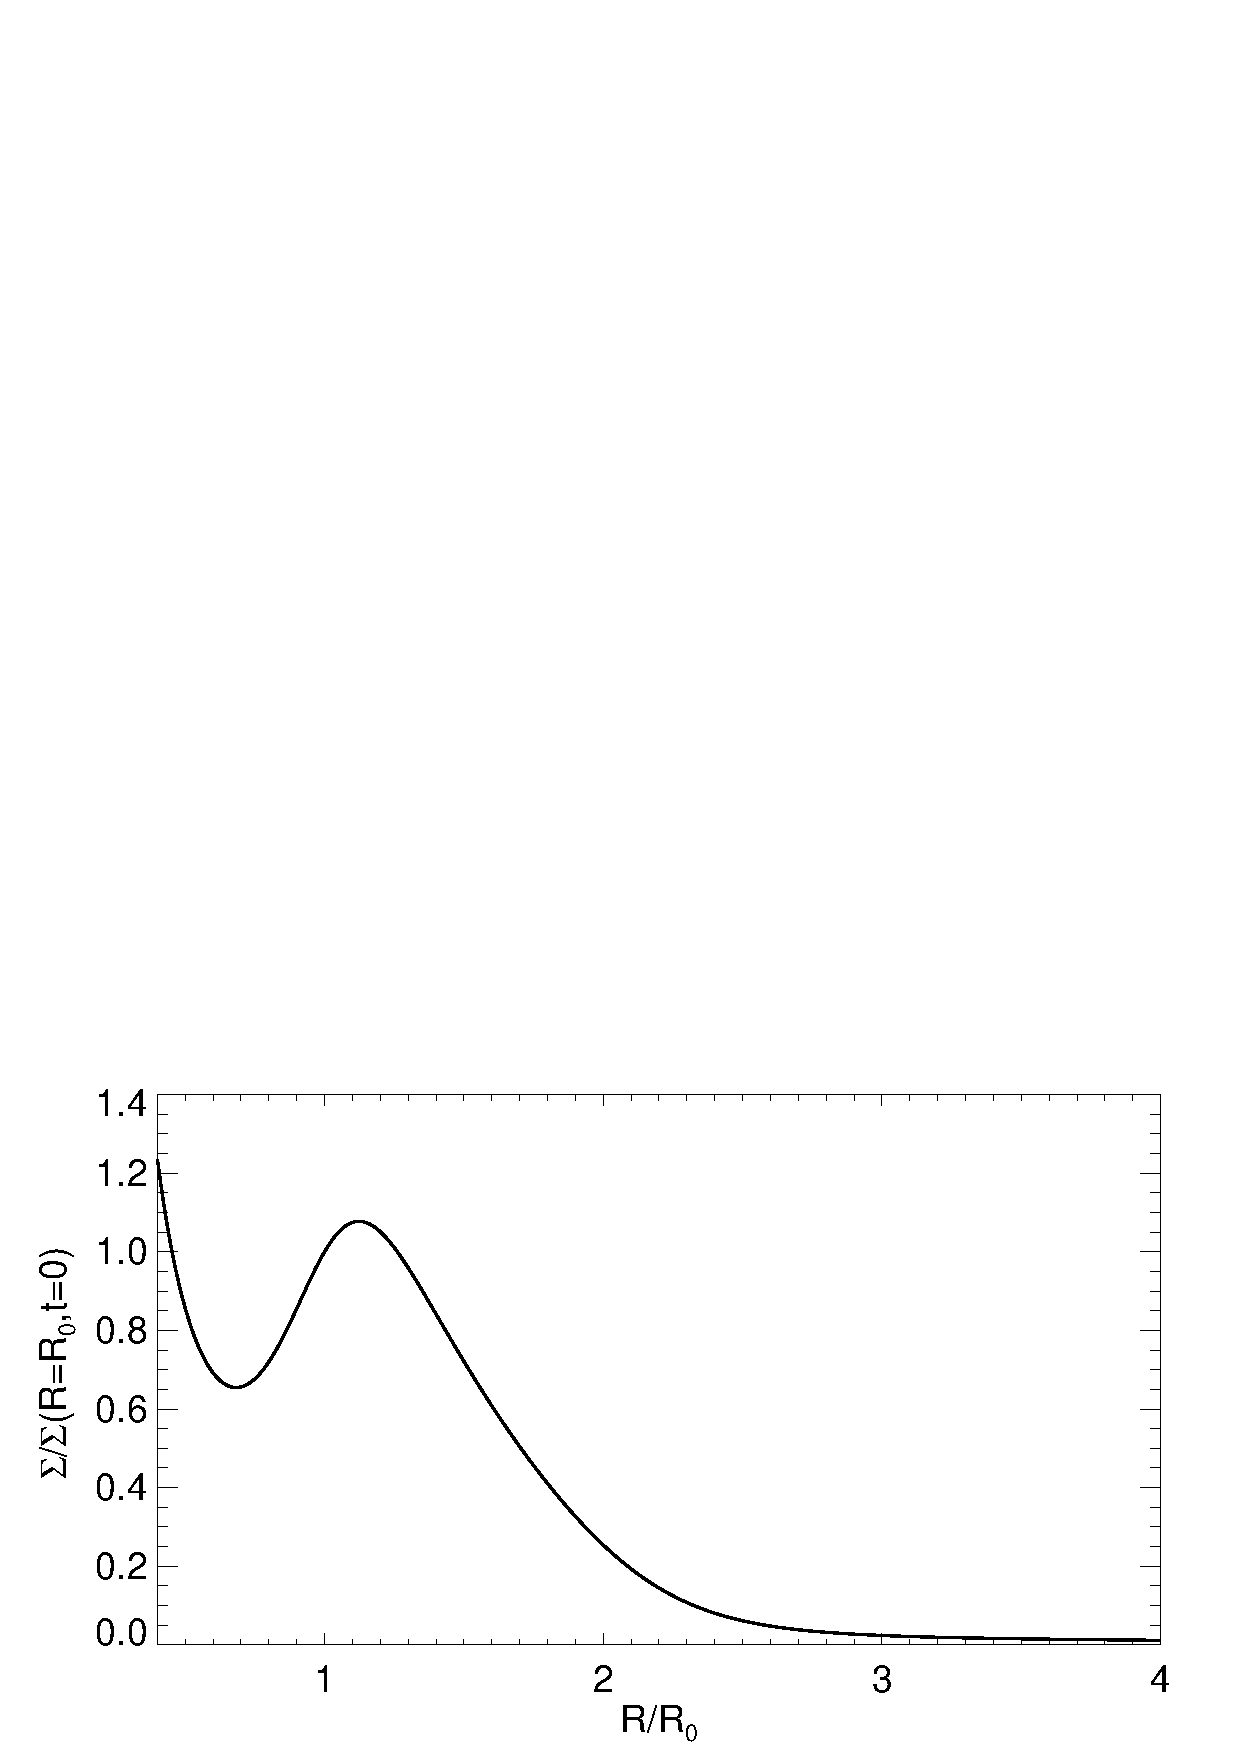
\includegraphics[width=\linewidth,clip=true,trim=0cm 1.7cm 0cm
  0cm]{figures/compare_profiles_dens000} 
  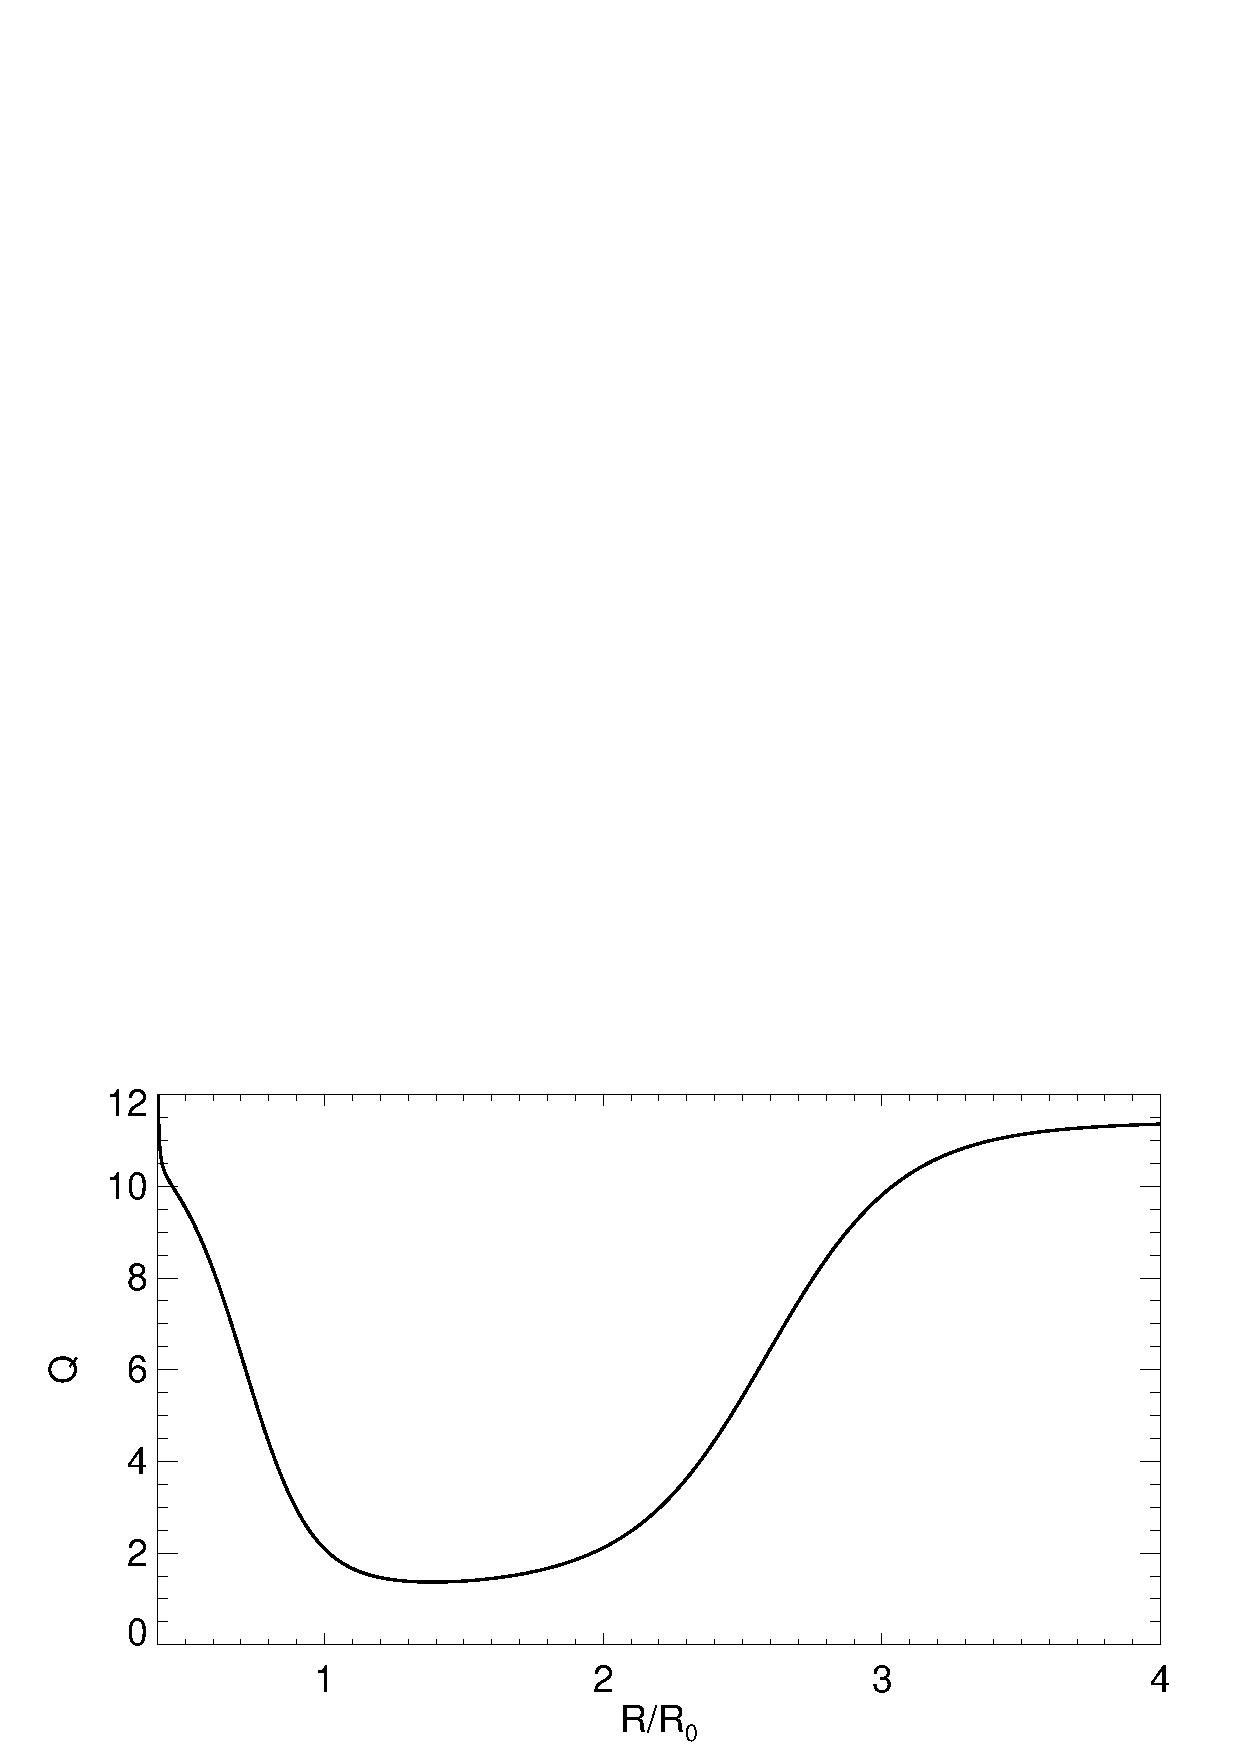
\includegraphics[width=\linewidth]{figures/compare_profiles_Q000}
  \caption{Fiducial profiles of the surface density (top) and Toomre
    parameter (bottom) used in this work.\label{initial_surf}}
\end{figure}


\section{Numerical methods}
%We will mostly employ 2D simulations in favour of resolution, but have
%also run some cases in 3D. We describe here the numerical setup used
%in each code. 
%introduce notation, terminlogy for each code 

We adopt computational units such that $G=M_*=R_0=1$. Time is measured
in the Keplerian orbital period at the reference radius, $P_0\equiv 
2\pi/\Omega_k(R_0)$.  

\subsection{FARGO}
Our primary code is FARGO with self-gravity \citep{baruteau08}. This
is a popular, simple finite-difference code for 2D discs. `FARGO' refers
to its azimuthal transport algorithm, which circumvents time-step
contraint set by the inner disc boundary. 
The 2D Poisson equation is solved in integral form 
\begin{align}\label{2d_grav}
  \Phi_{d,z=0}(R,\phi) = - \int
  \frac{G\Sigma(R^\prime,\phi^\prime)R^\prime dR^\prime d\phi^\prime}{\sqrt{R^2+R^{\prime 2} -
      2RR^\prime\cos{(\phi - \phi^\prime)} + \epsilon_g^2}} 
\end{align}
using Fast Fouier Transform (FFT), where $\epsilon_g$ is a softening
length to prevent a numerical singularity and the integration is taken
over the disc. The FFT approach requires
$\epsilon_g\propto R$ \citep{baruteau08}.  

The 2D disc occupies
$R\in[R_\mathrm{min},R_\mathrm{max}],\,\phi\in[0,2\pi]$ and is
divided into $(N_R,N_\phi)$ grids, logarithimically spaced in radius and
uniform spaced in azimuth. At radial boundaries we set the
hydrodynamic variables to their initial values.         

%poisson kernal integration, softening 
%where used?
%BC
\subsection{ZEUS-MP}
ZEUS-MP  is a general-purpose finite difference
code \citep{hayes06}. We use the code in 3D spherical geometry, covering
$r\in[r_\mathrm{min},r_\mathrm{max}]$, $\theta\in[\theta_\mathrm{min},\pi/2]$,
$\phi\in[0,2\pi]$. The vertical domain is chosen to cover $n_H$
scale-heights, i.e. $\tan{(\pi/2 - \theta_\mathrm{min})}/h=n_H$. 
The grid is logarithmically spaced in radius and uniformly spaced in the angular
coordinates. We assume reflectional symmetry across the midplane, and
apply relfective boundary conditions at radial boundaries and the
upper disc boundary.  

ZEUS-MP solves the 3D Poisson equation using a conjugate gradient
method. To suppliment boundary conditions for the linear solver, we
expand the boundary potential using in spherical harmonics $Y_{lm}$ 
as described in \cite{boss80}. The expansion is truncated at
$\lmax,\mmax$. This code was used in \cite{lin12b} for
self-gravitating disc-planet simulations.  

%used in lin 2012 
\subsection{PLUTO} 
PLUTO is a general-purpose Godunov code \citep{mignone07}. The grid
setup is the same as that adopted in ZEUS-MP above. We configure the
code similarly to that used in \cite{lin14}: piecewise linear
reconstruction, a Roe solver and second order Runge-Kutta time
integration. We also enable the FARGO algorithm for azimuthal
transport. 

We solve the 3D Poisson equation throughout the domain using spherical
harmonic expansion \citep{boss80}, as used for the boundary potential
in ZEUS-MP. This version of PLUTO was used in \cite{lin14b} for
self-gravitating disc-planet simulations, producing similar results to
that of ZEUS-MP and FARGO. 

%used in conference proceeding 

\subsection{Diagnostics}

\subsubsection{Evolution of non-axisymmetirc modes}
The disc evolution is quantified using mode amplitudes and angular
momenta as follows. We list the 2D definitions with obvious 3D generalisations. 
A hydrodynamic variable $f$ (e.g. $\Sigma$) is written as 
\begin{align}
  f(R,\phi,t) &= \sum_{m=-\infty}^{\infty}f_m(R,t)\exp{\ii m \phi} \notag\\
  &= f_0(R) + 2 \real\left[\sum_{m=1}^\infty f_m \exp{(\ii
      m\phi)}\right], 
\end{align}
where the $f_m$ may be obtained from Fourier transform in $\phi$. 

The normalised surface density associated with $m$ is
\begin{align}
  \Delta\Sigma_m = \frac{2}{\Sigma_{00}} \real\left[\Sigma_m \exp{(\ii
      m\phi)}\right]
\end{align}
where $\Sigma_{00} = \Sigma_0(t=0)$. The time evolution of the
$m^\mathrm{th}$ mode can be characterized by 
assuming $\Sigma_m\propto\exp{(-\ii \sigma t)}$, where
$\sigma = \omega + \ii\gamma$ is the complex frequency, $\omega$ is
the real frequency and $\gamma$ is the growth rate. The total
non-axisymmetric surface density is 
\begin{align}
  \Delta\Sigma = \frac{\Sigma - \Sigma_0}{\Sigma_0}. 
\end{align}


\subsubsection{Angular momentum decomposition}
The total disc angular momentum in $R\in[R_1,R_2]$ is
\begin{align}
  J &= \int_{R_1}^{R_2}\int_0^{2\pi} \Sigma Rv_\phi RdRd\phi \notag\\
  &= 2\pi\int_{R_1}^{R_2}R\Sigma_0 v_{\phi0} R dR \notag\\ 
  &\phantom{=}+
  \sum_{m=1}^\infty2\pi\int_{R_1}^{R_2} 2R\real\left[\Sigma_m v_{\phi
      m}^*\right] RdR, \notag\\
  &= \sum_{m=0}^\infty \int_{R_1}^{R_2}  j_m(R) dR = \sum_{m=0}^\infty J_m. 
\end{align}
where $^*$ denotes complex conjugation, and we idenfity $J_m$ as the 
angular momentum associated with disc structure with
$m^\mathrm{th}$-fold symmetry, and $j_m$ the associated angular
momentum per unit length. We will use $J_m$ to monitor angular momentum 
conservation for the disc as a whole.  

\section{Linear density waves}\label{wkb}
In this paper we take a fully numerical approach using non-linear
hydrodynamic simulations. However, it will be useful to employ
existing linear density wave theory to interpret the simulations. 
We list here the main definitions and results from 2D linear theory,
taken from \cite{lin11} and \cite{shu91}.  

In a linear analysis, one assumes a steady axisymmetric background state, such as
that defined in \S\ref{model}, which is then perturbed such that
\begin{align}  
  \Sigma \to \Sigma(R) + \delta\Sigma_m(R)\exp{\left[\ii\left(-\sigma t +
        m\phi\right)\right]}, 
\end{align}
and similarly for other variables. Since the background is
axisymmetric, we identify $\delta\Sigma_m(R)\exp{\left(-\ii\sigma
    t\right)} = \Sigma_m$ as defined for diagnostics. 
The linearised mass and momentum equations are
\begin{align}
  &-\ii\sbar \delta\Sigma_m = -\frac{1}{R}\frac{d}{dR}\left(R\Sigma\delta
    v_{Rm}\right) - \frac{\ii m \Sigma}{R}\delta v_{\phi m}, \\
  &-\ii\sbar\delta v_{Rm} - 2\Omega \delta v_{\phi m} = -
  c_s^2(R)\frac{d}{dR}\left(\frac{\delta\Sigma_m}{\Sigma}\right) - \frac{d}{dR}\delta\Phi_m,\\
  & -\ii\sbar\delta v_{\phi m} + \frac{\kappa^2}{2\Omega}\delta v_{Rm} =
  -\frac{\ii m }{R}\left(c_s^2\frac{\delta\Sigma_m}{\Sigma} + \delta\Phi_m\right),
\end{align}
where $\sbar = \sigma - m\Omega$ and $\kappa^2 =
R^{-3}\p_R(R^4\Omega^2)$ is the square of the epicycle frequency. A
locally isothermal equation of state has been assumed.    
The linearised Poisson equation is 
\begin{align}
  \nabla^2\delta\Phi_m = 4\pi G \delta\Sigma_m \delta(z). 
\end{align}

The linearised equations can be combined to a single
integro-differential eigenvalue problem. We list below some general
properties of the linear perturbations that will be useful for
understanding our simulations. We defer a full numerical
exploration of the linear problem to a future study. 

\subsection{Global angular momentum conservation for linear
  perturbations} 
It can be shown that linear perturbations with $\phi$-dependence in the form
$\exp{(\ii m\phi)}$ satisfies angular momentum conservation
in the form 
\begin{align} 
  \frac{\p \jlin}{\p t} + \nabla\cdot\bm{F} = \tbg, 
\end{align}
where
\begin{align}\label{lin_ang_mom_cons}
  \jlin \equiv
  -\frac{m\Sigma}{2}\imag\left(\bm{\xi}^*\cdot\frac{\p\bm{\xi}}{\p
      t} + \Omega \hat{\bm{k}}\cdot\bm{\xi}\times\bm{\xi}^* + \ii
    m \Omega |\bm{\xi}|^2\right) 
\end{align}
is the angular momentum density, $\bm{\xi}$ is the Lagragian
displacement, and $\bm{F}$ is the angular momentum flux
consisting of a Reynolds stress and a gravitational stress. Explicit
expressions for $\bm{\xi}$ and $\bm{F}$ can be found in e.g.,
\cite{papaloizou85} and \cite{lin11} respectively.   

The term $\tbg$ is 
\begin{align}\label{baroclinic_torque}
  \tbg \equiv
  -\frac{m}{2}\imag\left(\Sigma_m\xi_R^*\frac{dc_s^2}{dR}\right), 
\end{align}
and arises because we have adopted a locally isothermal equation of
state. In a barotropic fluid, such as a strictly isothermal disc,
$\tbg$ vanishes and the angular momentum associated with
the perturbation is conserved, provided that there is no net angular
momeumtum flux. We briefly outline the derivation of $T_\mathrm{BG}$
in Appendix 
\ref{tbg_deriv}. 

However, as noted in \cite{lin11}, if there is an imposed
temperature gradient, as is the disc models considered in this paper,
then $\tbg\neq 0$ in general, which corresponds to a torque
exerted by the background disc on the perturbation.       

We remark that the perturbed angular momentum density $\jlin$ has been
defined to satisfy a conservation law. This differs from the 
empirical angular momentum decomposition above. 

%each m satisfies its own equation 

\subsection{Local results}
%The linearised equations correspond to an integro-differential
%equation eigenvalue problem. 
In the local approximation, perturbations are assumed to vary rapidly
relative to any background gradients. \cite{shu91} gives the
dispersion relation for tightly-wound density 
waves of the form $\exp{[\ii(-\sigma t + m \phi + kR)]}$ in a razor-thin
disc as  
\begin{align}\label{dispersion}
  (\sigma - m\Omega)^2 = \kappa^2 + k^2c_s^2 - 2\pi G \Sigma |k|, 
\end{align}
and $k$ is a real wavenumber such that $|kR|\gg1$. Note that in this
approximation, only axisymmetric perturbations with $m=0$ can be
unstable (having an imaginary $\sigma$).  

Given the pattern speed $\Omega_p$, Eq. \ref{dispersion} can be solved
for $|k|$,   
\begin{align}\label{wavenumber}
  |k| = \frac{\pi G \Sigma}{c_s^2}\left[1 \pm \sqrt{1 -
      Q^2(1-\nu^2)}\right], 
\end{align}
where 
% \begin{align}
%   k_T \equiv \frac{\kappa^2}{2\pi G \Sigma}
% \end{align}
% is a characteristic wavenumber, 
\begin{align}
  Q \equiv \frac{c_s\kappa}{\pi G \Sigma}
\end{align}
is the usual Toomre parameter, and
\begin{align}
  \nu \equiv \frac{(\omega - m\Omega)}{\kappa}
\end{align}
is a dimensionless frequency. The upper (lower) signs in
Eq. \ref{wavenumber} correspond to short (long) waves.  

The \emph{co-rotation radius} $R_c$ is where the pattern speed matches
the fluid rotation,
\begin{align}
  \Omega(R_c) = \Omega_p.
\end{align}
\emph{Lindblad resonances} $R_L$ occurs where
\begin{align}
  \nu^2(R_L) = 1. 
\end{align}
Finally, \emph{Q-barriers} occur at radii $R_{Qb}$ where
\begin{align}
  Q^2(R_{Qb})\left[1-\nu^2(R_{Qb})\right] = 1.  
\end{align}
According to Eq. \ref{wavenumber}, purely wave-like solutions with
real $k$ are only possible when $Q^2(1-\nu^2)\leq1$.  

A detailed discussion of the properties of density waves in the local
approximation can be found in \cite{shu91}. A important result is that
waves interior to co-rotation ($R<R_c$) have negative angular momentum, while
waves outside co-rotation ($R>R_c$) have positive angular
momentum. The local approximation becomes less good for gobal modes,
but will nevertheless be useful in results interpretation.   

\section{Results}\label{results2d}
We first present results from FARGO simulations. The 2D disc spans
$[R_\mathrm{min}, R_\mathrm{max}] = [0.4,10]R_0$. This gives a total
disc mass $M_{d}=0.086M_*$. The mass within
$R\in[R_\mathrm{min},R_{1}]$ is $0.017M_*$, that within
$R\in[R_{1},R_{2}]$ is $0.049M_*$, and that within
$R\in[R_{2},R_\mathrm{max}]$ is $0.021M_*$. We use a resolution of
$N_R\times N_\phi = 1024\times 2048$, or about $16$ grids per $H$, and
adopt $\epsilon_g=10^{-4}hR$ for the   
self-gravity softening length\footnote{In 2D self-gravity, $\epsilon_g$ also
  approximates for the vertical disc thickness, so a more appropriate
  value would be $\epsilon_g\sim H$ \citep{muller12}. However, because
  $\epsilon_g\propto R$ is needed in FARGO, the Poisson kernel
  (Eq. \ref{2d_grav}) is no longer symmetric in $(R,R^\prime)$. We
  choose a small  
  $\epsilon_g$ in favour of angular momentum conservation, keeping in
  mind that the strength of self-gravity will be over-estimated.}.

In these simulations the disc is subject to initial perturbations in 
cylindrical radial velocity, 
\begin{align}\label{randpert}
  v_R \to v_R+ c_s\frac{\delta}{M}
  \exp{\left[-\frac{1}{2}\left(\frac{R-\overline{R}}{\Delta 
          R}\right)^2\right]}\sum_{m=1}^M\cos{m\phi},
\end{align}
where the amplitude $\delta\in[-10^{-3},10^{-3}]$ is set randomly but
independent of $\phi$, $\overline{R} = (R_{1}+R_{2})/2$
and $\Delta R = (R_{2}-R_{1})/2$. 

\subsection{Reference run}
To obtain a picture of the overall disc evolution, we describe a 
fiducial run initialised with $M=10$ in Eq. \ref{randpert}. 
Fig. \ref{fargo_modeamp} plots evolution of the maximum 
non-axisymmetric surface density amplitudes in $R\in[R_{1},R_{2}]$
for $m\in[1,10]$. Snapshots from the simulation are shown in
Fig. \ref{fargo_2d}. 
At early times $t\lesssim100P_0$ the disc 
dominated by low-amplitude high-$m$ perturbations. The $m\geq4$ modes
growth initially and saturate (or decays) after $t=40P_0$. Notice the
low $m\leq 2$ modes decay initially, but grows between $t\in[20,40]P_0$,
possibly due to non-linear interaction of the high-$m$ modes  
\citep{laughlin96,laughlin97}. However, the $m=1$ mode begins to grow
again after $t=70P_0$, and eventually dominates the annulus. 

\begin{figure}
  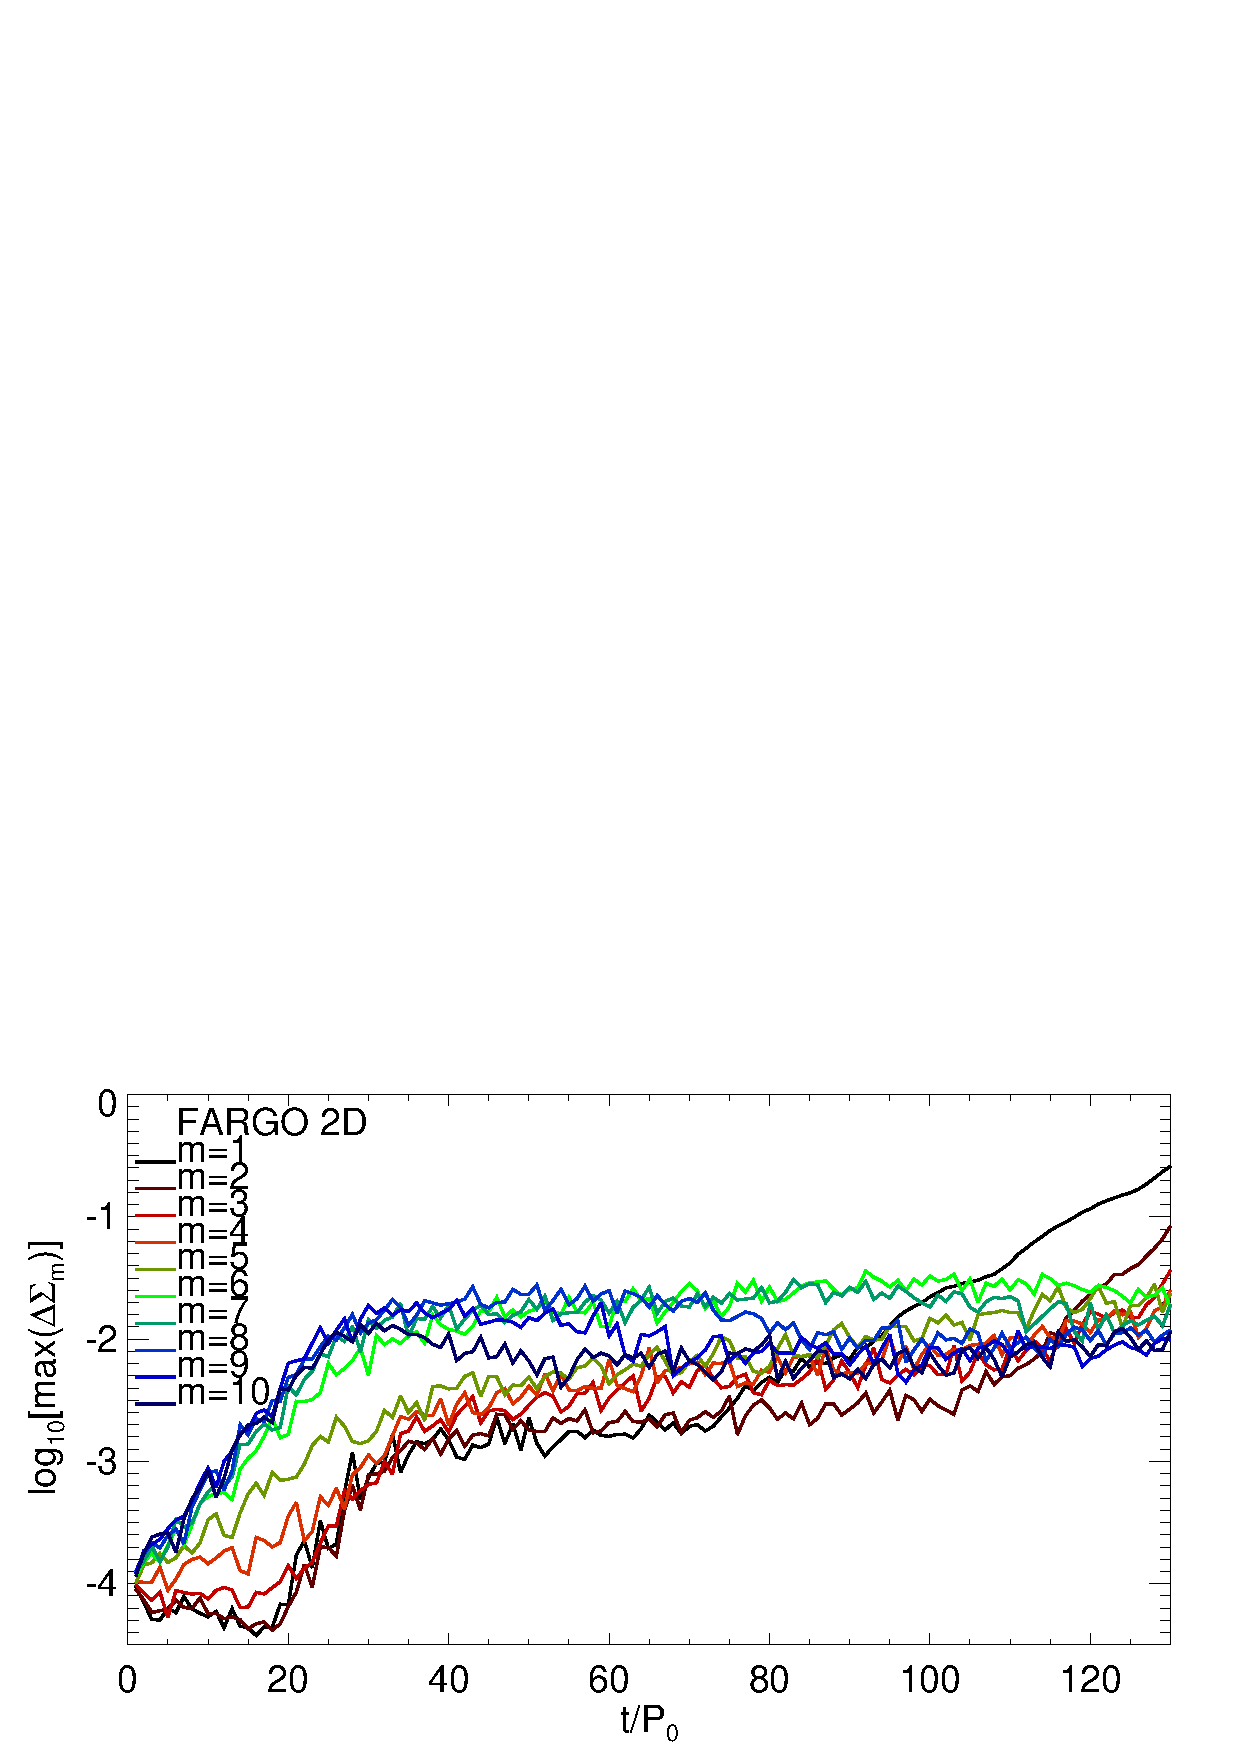
\includegraphics[width=\linewidth]{figures/nonaxi_evol_DZ_fargo}
  \caption{Evolution of non-axisymmetric surface density maxima 
    in the FARGO simulation initialised with perturbations
    with $m\in[1,10]$.\label{fargo_modeamp}} 
\end{figure}

\begin{figure}
  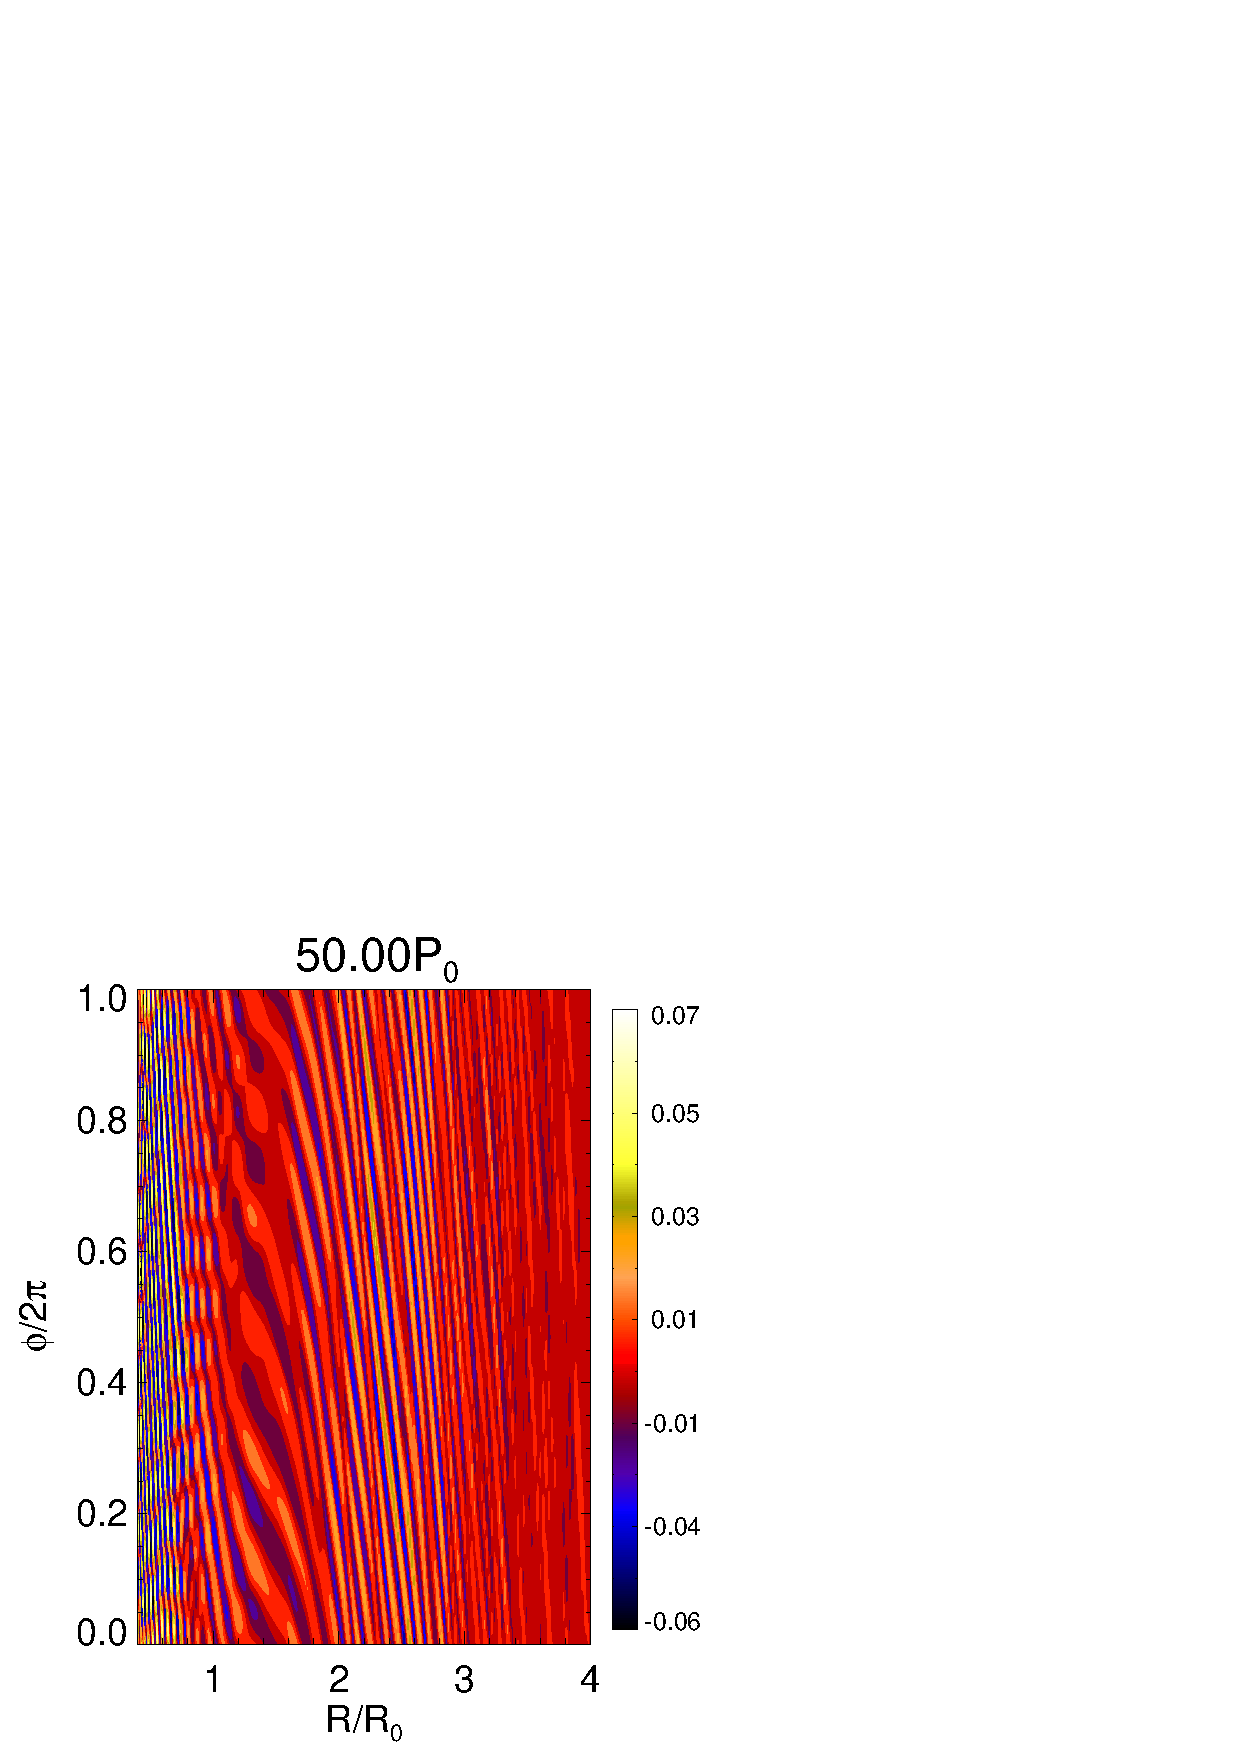
\includegraphics[scale=0.27]{figures/polarxy_dens050}\includegraphics[scale=0.27,clip=true,trim=2.26cm 
  0cm 0cm 
  0cm]{figures/polarxy_dens110}\includegraphics[scale=0.27,clip=true,trim=2.26cm
  0cm 0cm 0cm]{figures/polarxy_dens130} 
  \caption{Visualisation of the FARGO 2D simulation in
    Fig. \ref{fargo_modeamp}. The total  
    non-axisymmetric surface density
    $\Delta\Sigma$ is shown. \label{fargo_2d}} 
\end{figure}

Fig. \ref{2d_angmom} shows the evolution of disc angular momentum
components. Only the $m=0,\,1$ components are 
plotted since they are dominant. The $m=1$ structure has
an associated negative angular momentum.  
Its growth is compensated by an increase in the axisymmetric
component of angular momentum, such that $\Delta J_0 + \Delta
J_1 \sim 0$. Note that FARGO does not conserve angular momentum
exactly. However, we find the total angular momentum varies by 
$|\Delta J/J|= O(10^{-6})$, and is much smaller than the
change in the angular momenta components, $|\Delta J_{0,1}/J|>
O(10^{-5})$. Fig. \ref{2d_angmom} then suggest that angular momentum
is transferred from the one-armed spiral to the background disc.    

\begin{figure}
  % scale=0.41
  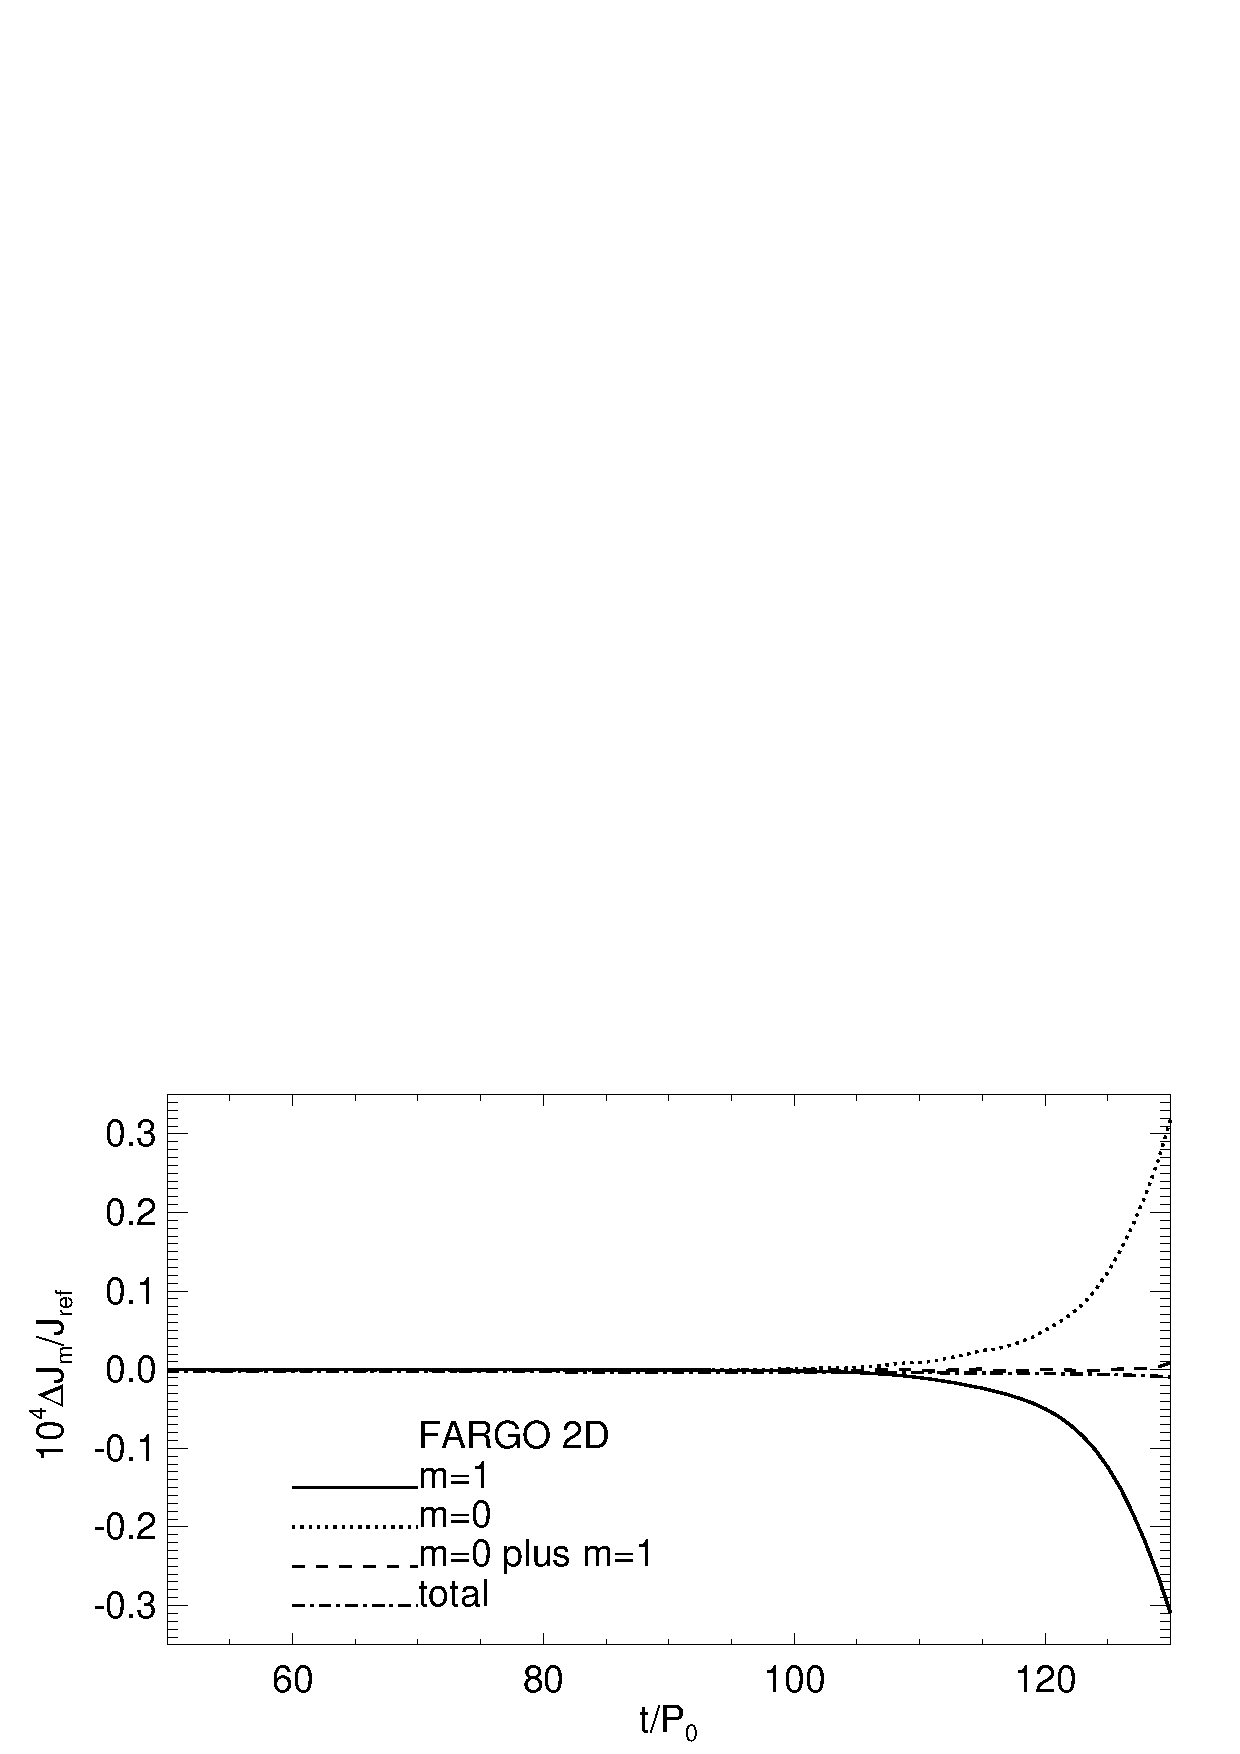
\includegraphics[width=\linewidth]{figures/nonaxi_evol_ang_fargo}
  \caption{Evolution of angular momentum components in the 
    FARGO simulation in Fig. \ref{fargo_modeamp}---\ref{fargo_2d}. The
    perturbation relative to $t=0$ in 2D is shown in units of the 
    initial total angular momentum $J_\mathrm{ref}$.\label{2d_angmom}} 
\end{figure}   

\subsection{Properties of the $m=1$ spiral and its growth}\label{fargo_m1}
In order to characterise the $m=1$ spiral that eventually
dominates, here we examine a simulation initialised with 
$M=1$ in Eq. \ref{randpert}. The one-armed spiral that emerges is more
coherent than the above simulation, which facilitates the analysis
below.   

Fig. \ref{2d_fargo_viz} shows a snapshot of the $m=1$ surface
density. By measuring the $m=1$ surface density amplitude and its
pattern speed, we obtain a co-rotation radius and growth rate 
\begin{align*}
  &R_c \simeq 4.4R_0,\\
  &\gamma\simeq 0.014\Omega_k(R_0) = 0.13\Omega_p. 
\end{align*}
This one-armed spiral can be considered as low frequency because its 
pattern speed $\Omega_p \simeq 0.1\Omega_k(R_0)\lesssim 0.3\Omega$ in
$R\in[R_{1},R_{2}]$ (where it has the largest amplitude). Thus, the spiral 
pattern appears nearly stationary. The growth rate $\gamma$ is also slow
relative to the local rotation, although the characteristic growth
time $\gamma^{-1} \simeq 10P_0$ is not very long.  
\begin{figure}
  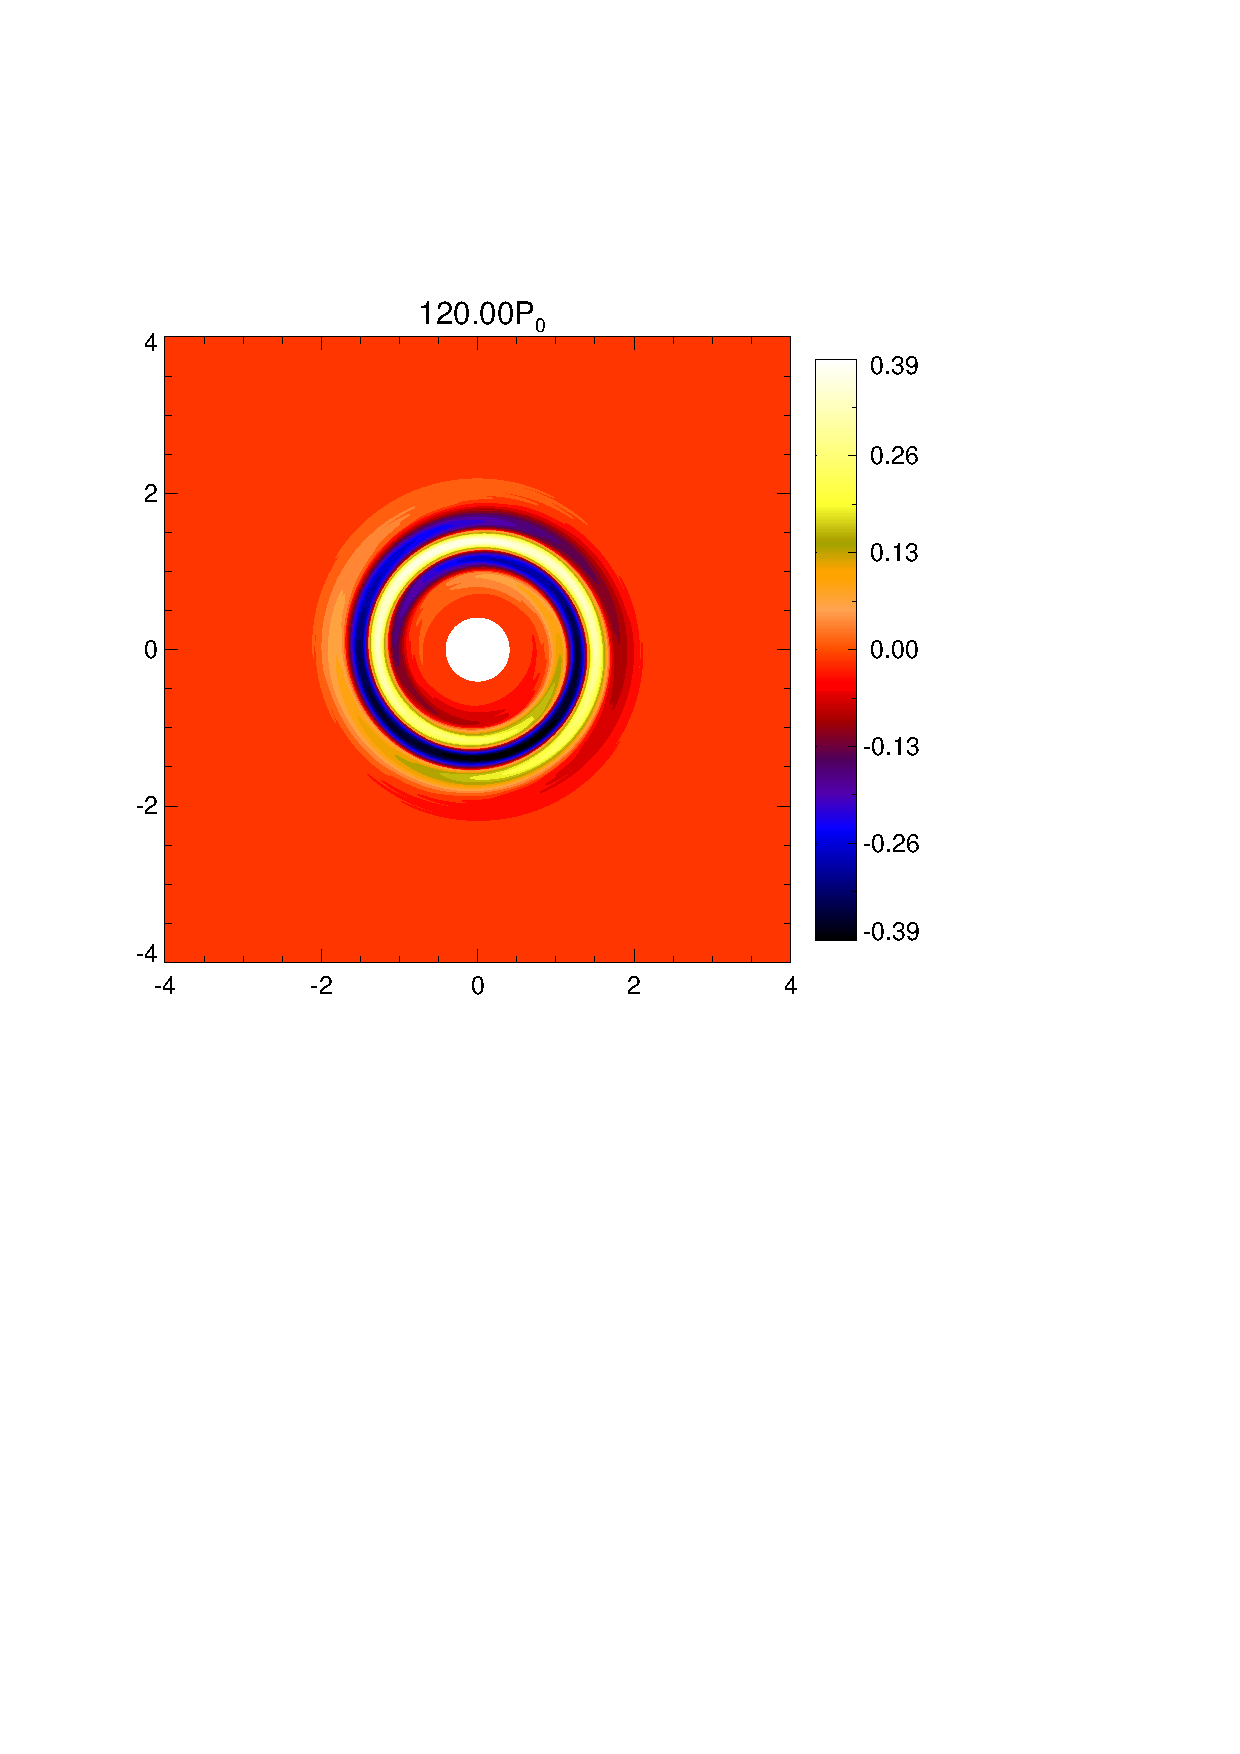
\includegraphics[width=\linewidth]{figures/polarxy2_dens120_fargo}
  \caption{Cartesian visualisation of the $m=1$ surface density
    structure in the FARGO simulation initialised with only $m=1$
    perturbations. 
    \label{2d_fargo_viz}} 
\end{figure}   

Next, we write $\Sigma_1 = 
|\Sigma_1|\exp{(\ii kR)}$, where $k$ is real, and assume the amplitude
$|\Sigma_1|$ varies slowly compared to the complex phase. This is the
main assumption in local theory. We calculate $k$ numerically and plot
its normalised value in Fig. \ref{fargo_wavenumber}. We find 
\begin{align*}
  kR \sim \frac{\pi G \Sigma}{c_s^2}R \sim \frac{1}{hQ}, 
\end{align*}
where we used $Q\sim c_s\Omega/\pi G \Sigma$ and $R\Omega/c_s\sim
h^{-1}$. Since $Q=O(1)$ and $h\ll 1$ imply $|kR|\gg 1$, we 
can apply results from local theory
self-consistently. Fig. \ref{2d_fargo_viz} shows the $m=1$ spiral is
trailing, which is consistent with $k>0$. 
 
%snapshot shows it's tightly wound
\begin{figure}
  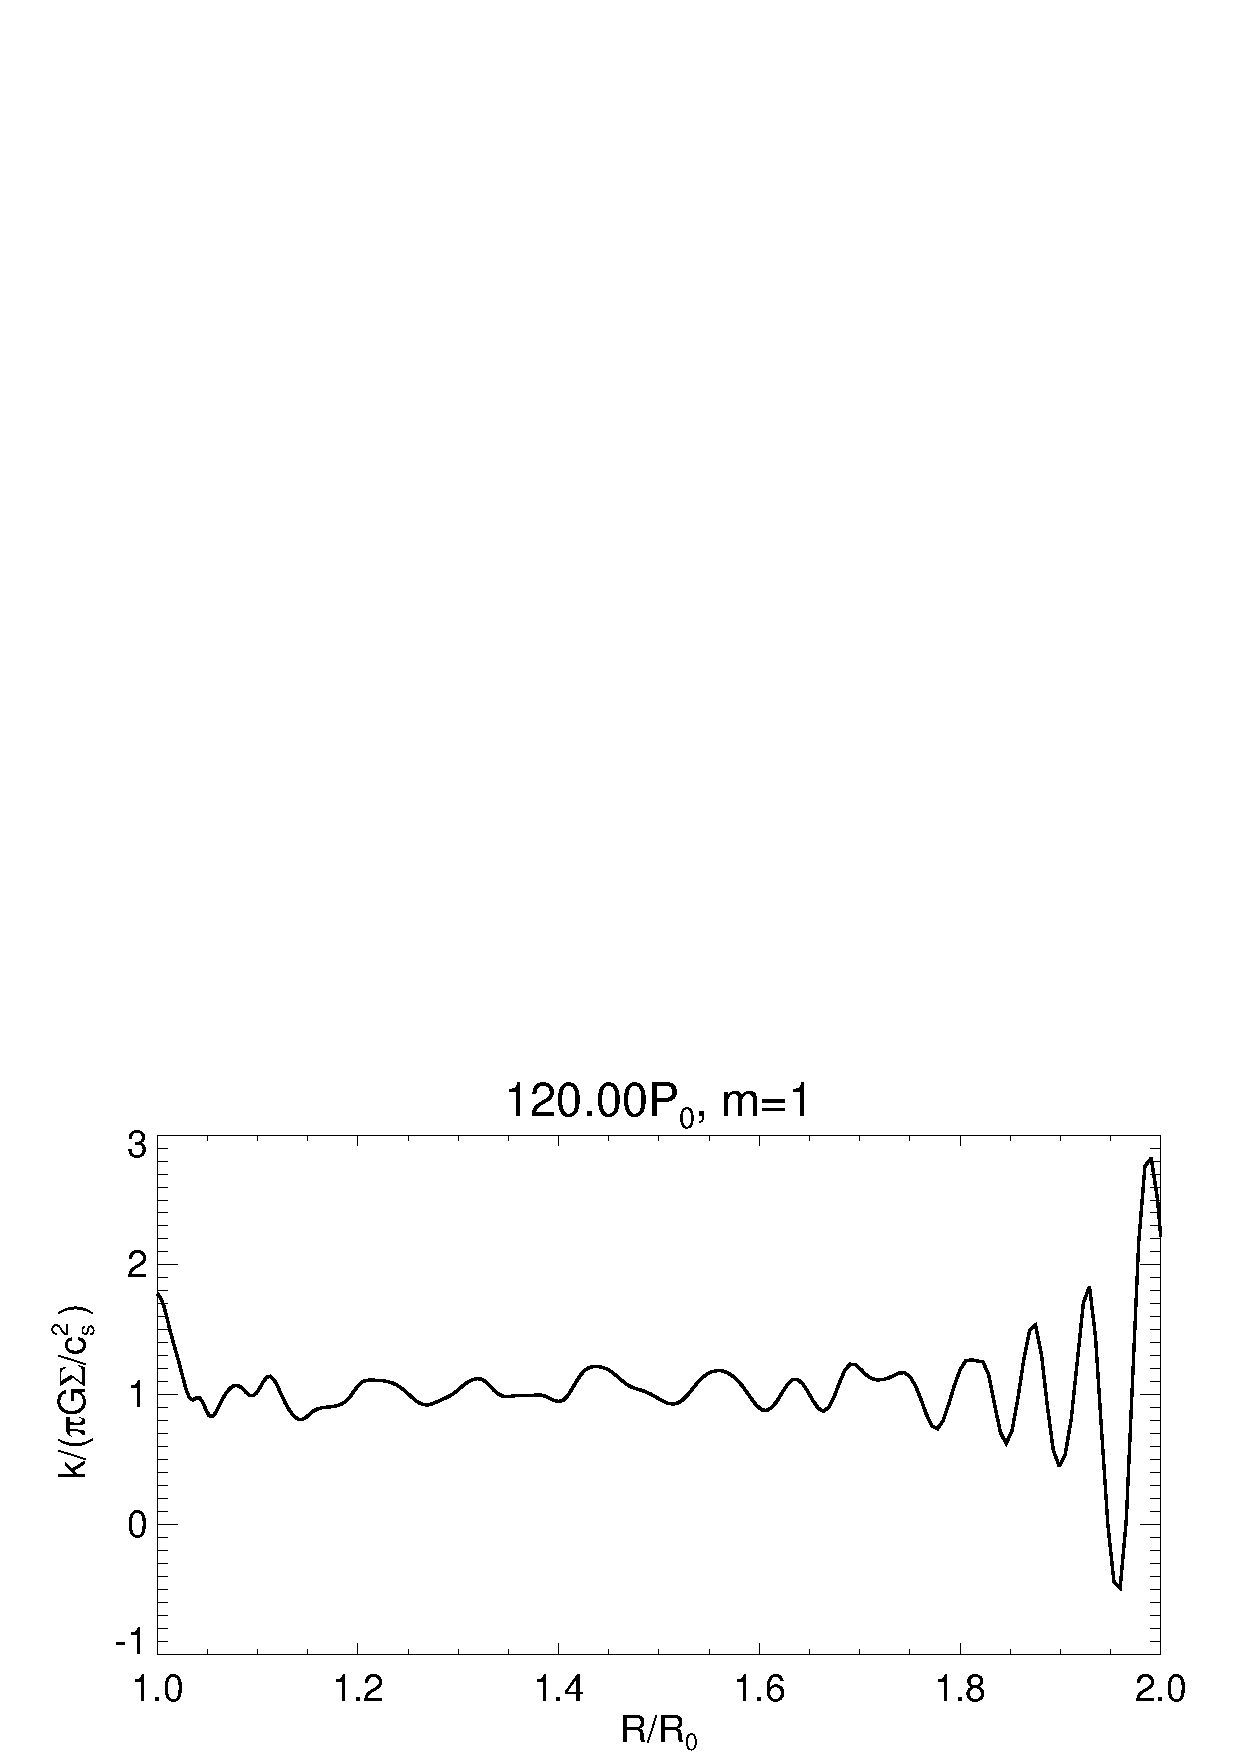
\includegraphics[width=\linewidth]{figures/m1_analysis_kr120_fargo}
  \caption{Normalised radial wavenumber of the $m=1$ spiral in 
    Fig. \ref{2d_fargo_viz}.\label{fargo_wavenumber}} 
\end{figure}   

%%%%%%%%%%%%%%%%%%%%%% 

Using the estimated value of $R_c$, we plot in
Fig. \ref{fargo_qbarrier} the quantity $\nu^2 - 1 + Q^{-2}$, which is
required to be positive in local theory for purely wave-like
solutions to the dispersion relation (Eq. \ref{dispersion}) when the
mode frequency is given. %Note that, with the above measured wavenumber $k$, 
%Eq. \ref{dispersion} requires $\nu^2 - 1 + Q^{-2}\sim0$ and the lower
%sign (long waves) to be taken. 
Fig. \ref{fargo_qbarrier} shows two $Q$-barriers located in
the inner disc, at $R_{Qb}=R_0$ and $R_{Qb}=1.6R_0$; the bounded region is indeed 
where the $m=1$ spiral develops. This suggests that the one-armed 
spiral is trapped. Note in this region, $\nu^2 - 1 + 
Q^{-2}\simeq 0.1\ll 1$, which is necessary for consistency with 
the measured wavenumber $k$ and Eq. \ref{wavenumber}.  
%Eq. \ref{dispersion} with the lower sign taken (i.e. long waves).  
There is one outer Lindblad resonance at $R_L\simeq
7.2R_0$. Thus, acoustic waves may be launched in $R\gtrsim 7.2R_0$ by
the spiral disturbance in the inner disc \citep{lin11b}. 
%implications: effect on dynamics in outer disc 

\begin{figure}
  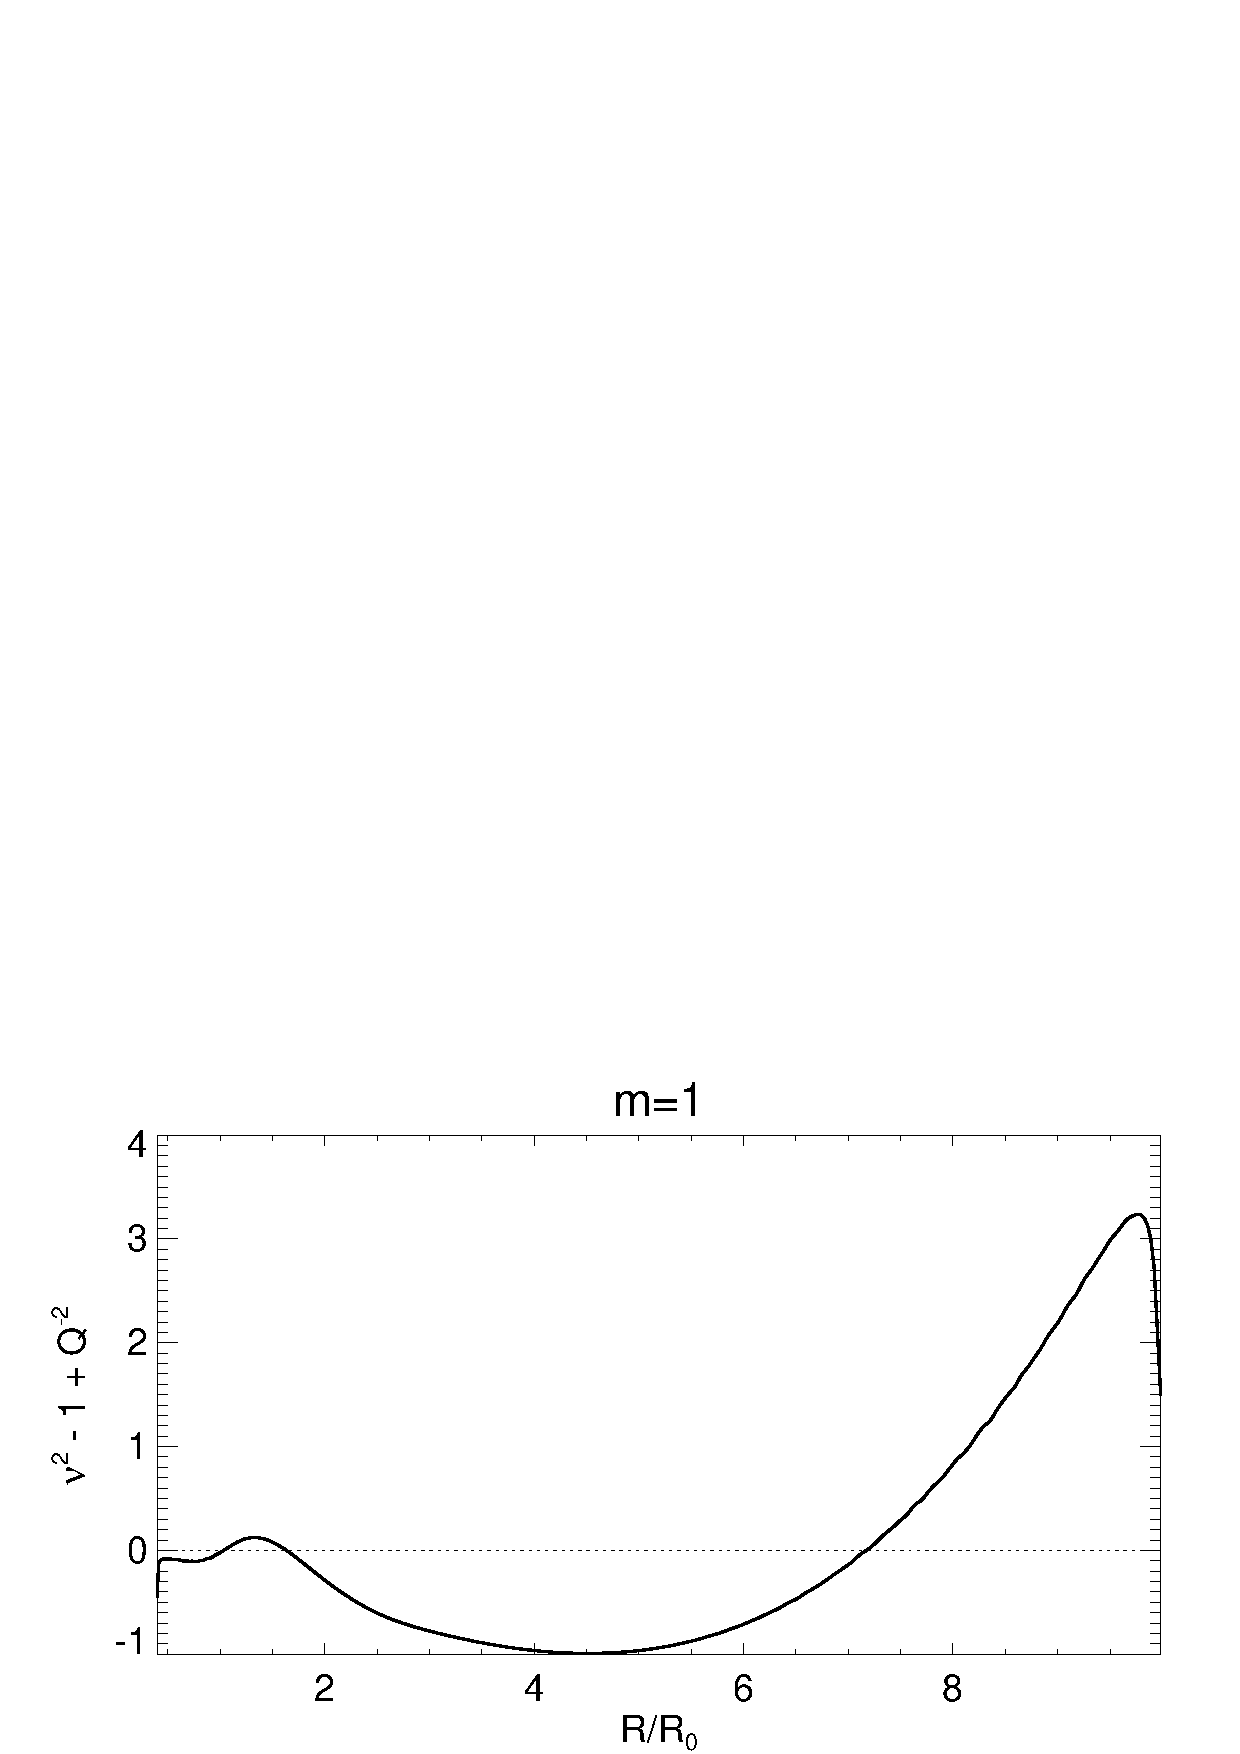
\includegraphics[width=\linewidth]{figures/m1_analysis_Qbar_fargo} 
  \caption{Dimensionless mode frequency $\nu$ for the $m=1$ spiral in
    Fig. \ref{2d_fargo_viz}. For a given real mode frequency, the
    dispersion relation for local density waves, Eq. \ref{dispersion},
    permits purely wave-like solutions in regions where $\nu^2 - 1 +
    Q^{-2}>0$.    
    \label{fargo_qbarrier}} 
\end{figure}

\subsubsection{Angular momentum exchange with the background disc}  
The wavenumber $k = \pi G\Sigma/c_s^2$ minimises the shifted frequency
$\sbar$ in the dispersion relation, Eq. \ref{dispersion}.  
Physically, then, it is not surprising to 
find perturbations of this wavenumber in a
self-gravitating disc where $Q\sim 1$. However, according the
local dispersion relation, $m=1$ perturbations are
formally stable for real $k$ and $Q>1$.   

%most of the perturbation is inside co-rotation 
%so resonant interaction unlikely for instability 

In order to track down the origin for the (slow) growth of the
$m=1$ spiral, we invoke angular momentum conservation for linear
perturbations, Eq. \ref{lin_ang_mom_cons}. Assuming fluxes are
negligible at the disc boundaries, we can integrate
Eq. \ref{lin_ang_mom_cons} to give
\begin{align}\label{baroclinic_torque_int}
  \frac{d}{dt}\underbrace{\int_{R_\mathrm{min}}^{R_\mathrm{max}}\jlin
    2\pi R dR}_{\jlintot} 
  =\int_{R\mathrm{min}}^{R\mathrm{max}}T_\mathrm{BG} 2\pi R dR, 
\end{align}
where we recall $T_\mathrm{BG}$ is the torque density due to the imposed
sound-speed profile (Eq. \ref{baroclinic_torque}). We explicitly 
compute both sides of Eq. \ref{baroclinic_torque_int} using
simulation data, and compare them in Fig. \ref{fargo_angmom_ex}. There
is a good match between the two torques, especially at early times
$t\lesssim110P_0$. The average discrepancy is $\simeq 5\%$. 
The match is less good later on, when the spiral
amplitude is no longer small ($\Delta\Sigma_1\sim 0.2$ at $t=110P_0$
and $\Delta\Sigma_1\sim 0.4$ by $t=120P_0$) and linear theory becomes
less applicable. Fig. \ref{fargo_angmom_ex} confirms that the $m=1$ spiral
wave experiences a negative torque that further reduces its angular
momentum. This is consistent with angular momentum component
measurements (Fig. \ref {2d_angmom}).  

% similar results if only intergrating between R_1 and R_2
%wave losses at boundaries 

\begin{figure}
  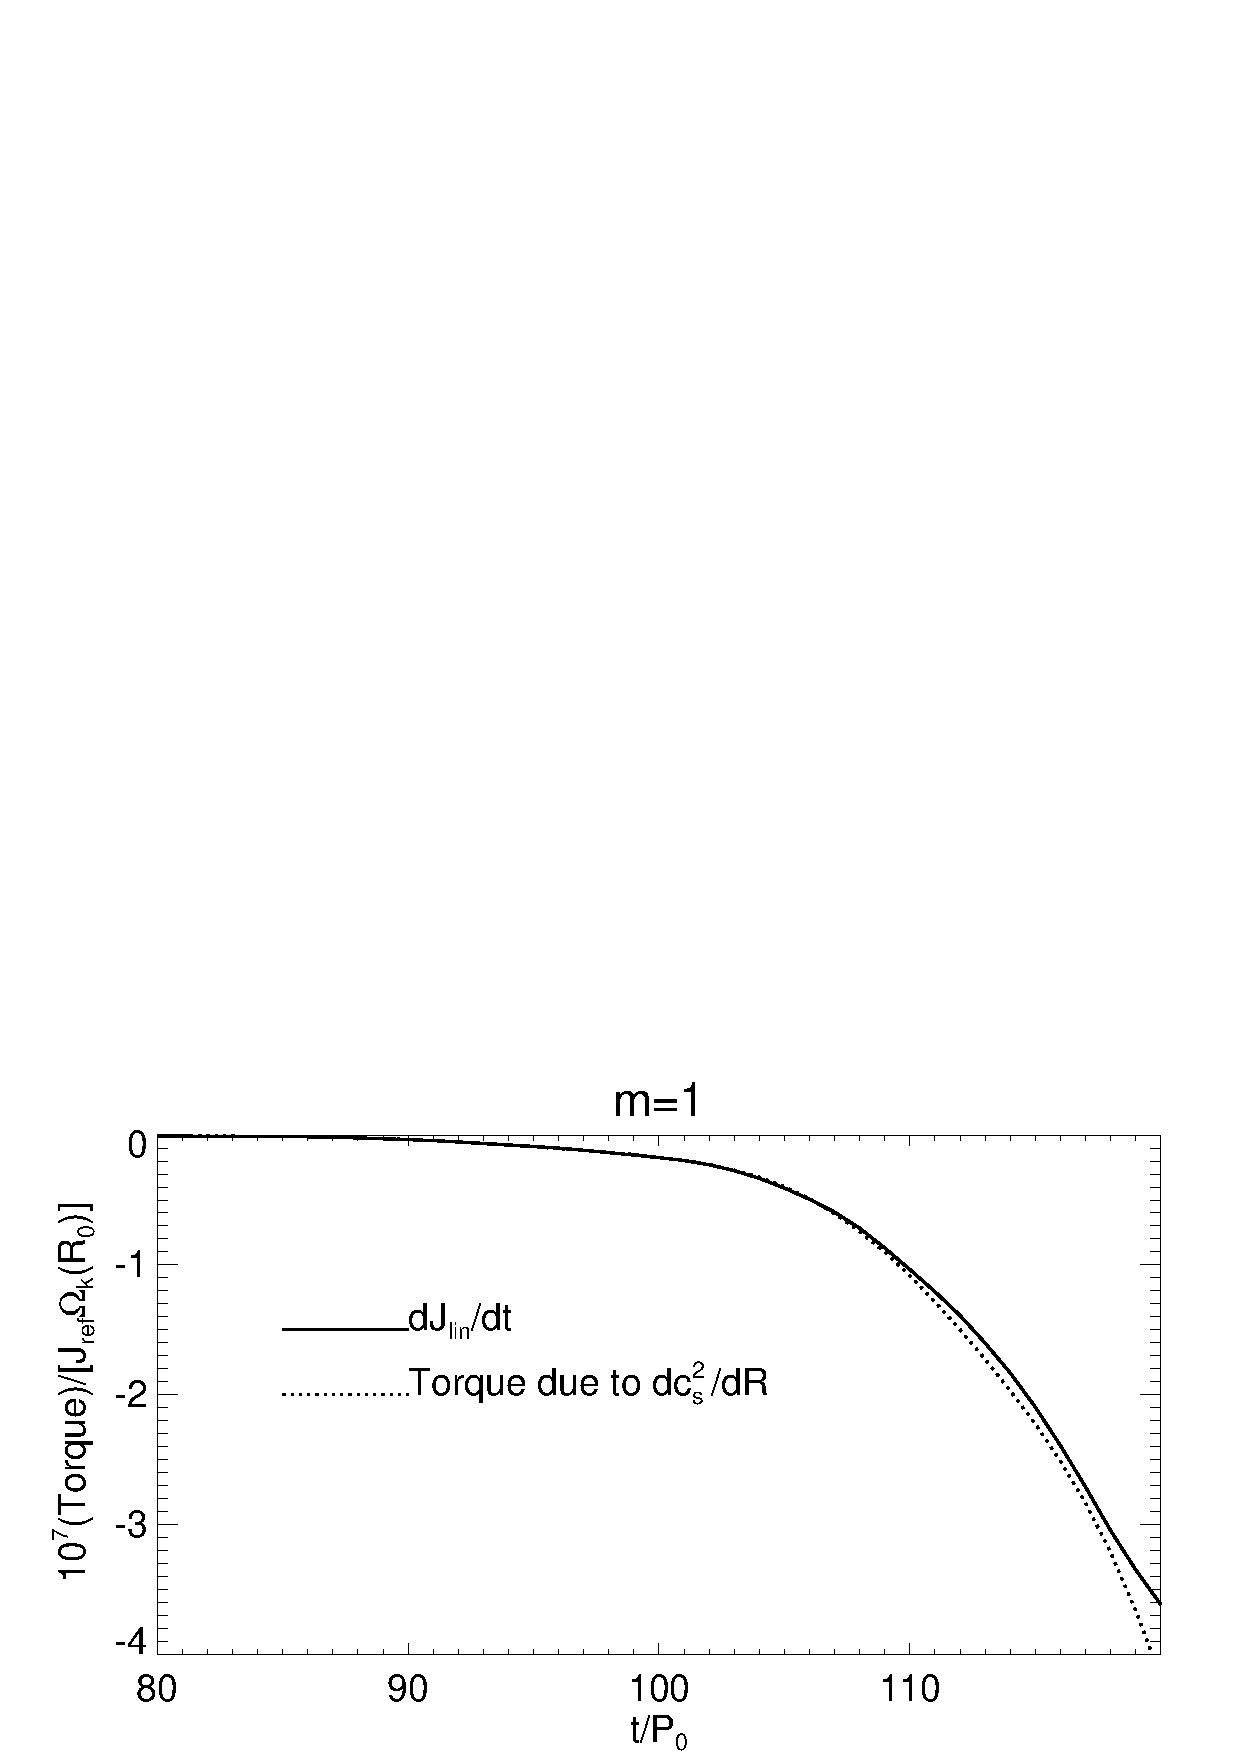
\includegraphics[width=\linewidth]{figures/m1_analysis_ang_fargo} 
  \caption{Rate of change of the $m=1$ wave angular momentum as defined by
    Eq. \ref{baroclinic_torque_int} (solid) compared to the torque
    exerted on the wave associated with the background temperature
    gradient (dotted). 
    \label{fargo_angmom_ex}} 
\end{figure}

%ang mom decreases slightly more rapidly than torque exchange provides
%- probably non-linear effects/shocks 

\subsection{Dependence on the imposed temperature profile}
The simulations above suggest the growth of the $m=1$ spiral mode
can be attributed to the background torque applied on linear perturbations
as a result of an imposed temperature gradient, as discussed in
\S\ref{global_cons}. According to Eq. \ref{baroclinic_torque}, this
torque is proportional to $q$, the power-law index used to set the
sound-speed profile (Eq. \ref{sound-speed}) in our simulations. 
We confirm this through a series of simulations with $q\in[0,1]$, 
initialised with $m=1$ perturbations. However, to keep the Toomre $Q$
profiles similar, we adjust the surface density power-law index such
that $s = (3+q)/2$.  

Fig. \ref{fargo_varq} compares the $m=1$ spiral amplitudes as a
function of $q$. We indeed observe slower growth with decreasing
$q$. Although the figure indicates growth for the strictly isothermal
disc ($q=0$), we did not observe a coherent one-armed spiral upon
inspection of the $m=1$ surface density field. The growth in this case
may be associated with high-$m$ modes, which dominated the
simulation.   

% difficult to measure  
% show result of isothermal calc?

\begin{figure}
  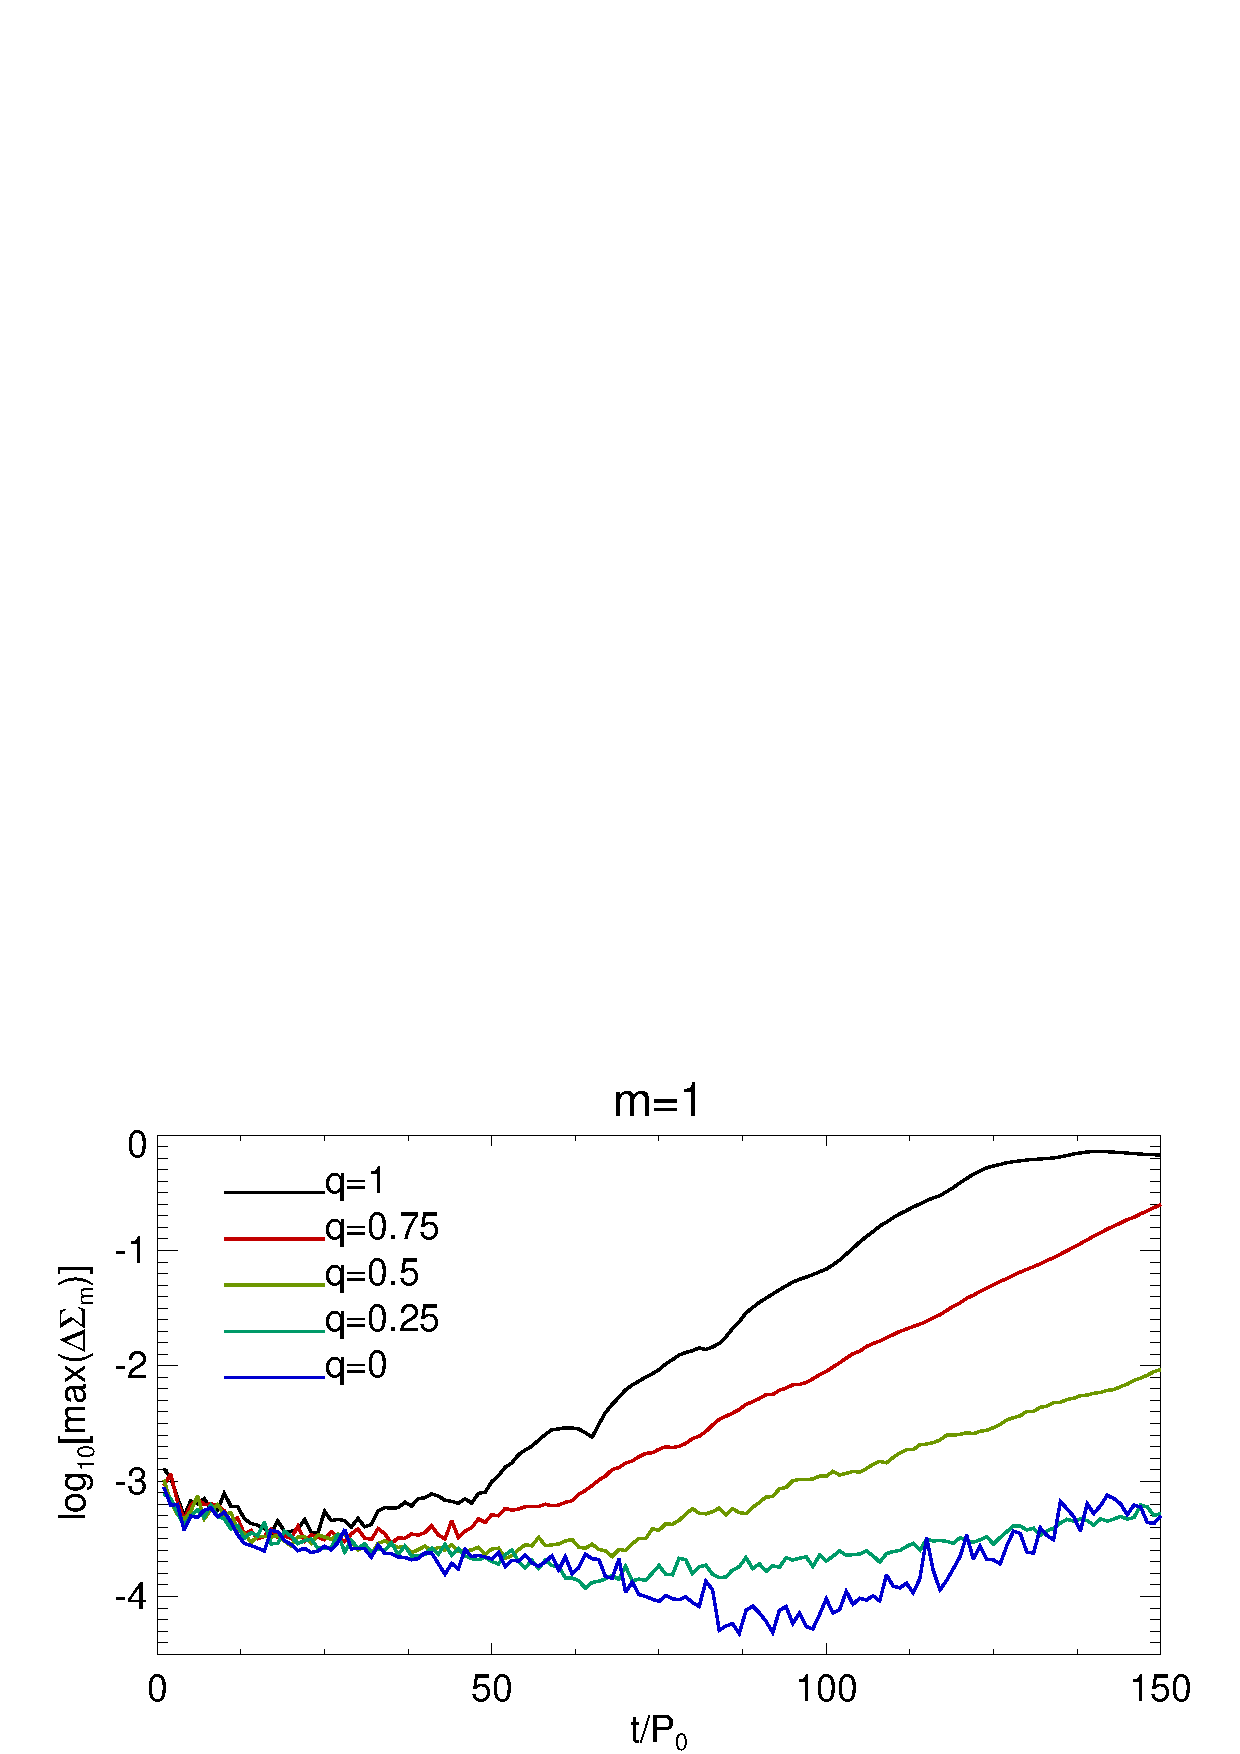
\includegraphics[width=\linewidth]{figures/m1_analysis_plot_fargo_varq}   
  \caption{Evolution of the $m=1$ spiral amplitude as a function of
    the imposed sound-speed gradient $q$. The maximum value of the
    $m=1$ surface density in $R\in[R_1,R_2]$ is shown. 
    \label{fargo_varq}} 
\end{figure}
We plot growth rates of the $m=1$ spiral as a function of $q$ in 
Fig. \ref{fargo_varq_growth}. The correlation can be fitted with a 
linear relation
\begin{align*}
  \gamma \simeq \left[0.015 q - 7.9\times10^{-4}\right] \Omega_k(R_0). 
\end{align*}
% difficult to measure very small growth rates
This shows that the temperature gradient is responsible for the
development of the one-armed spirals observed in our simulations.  

\begin{figure}
  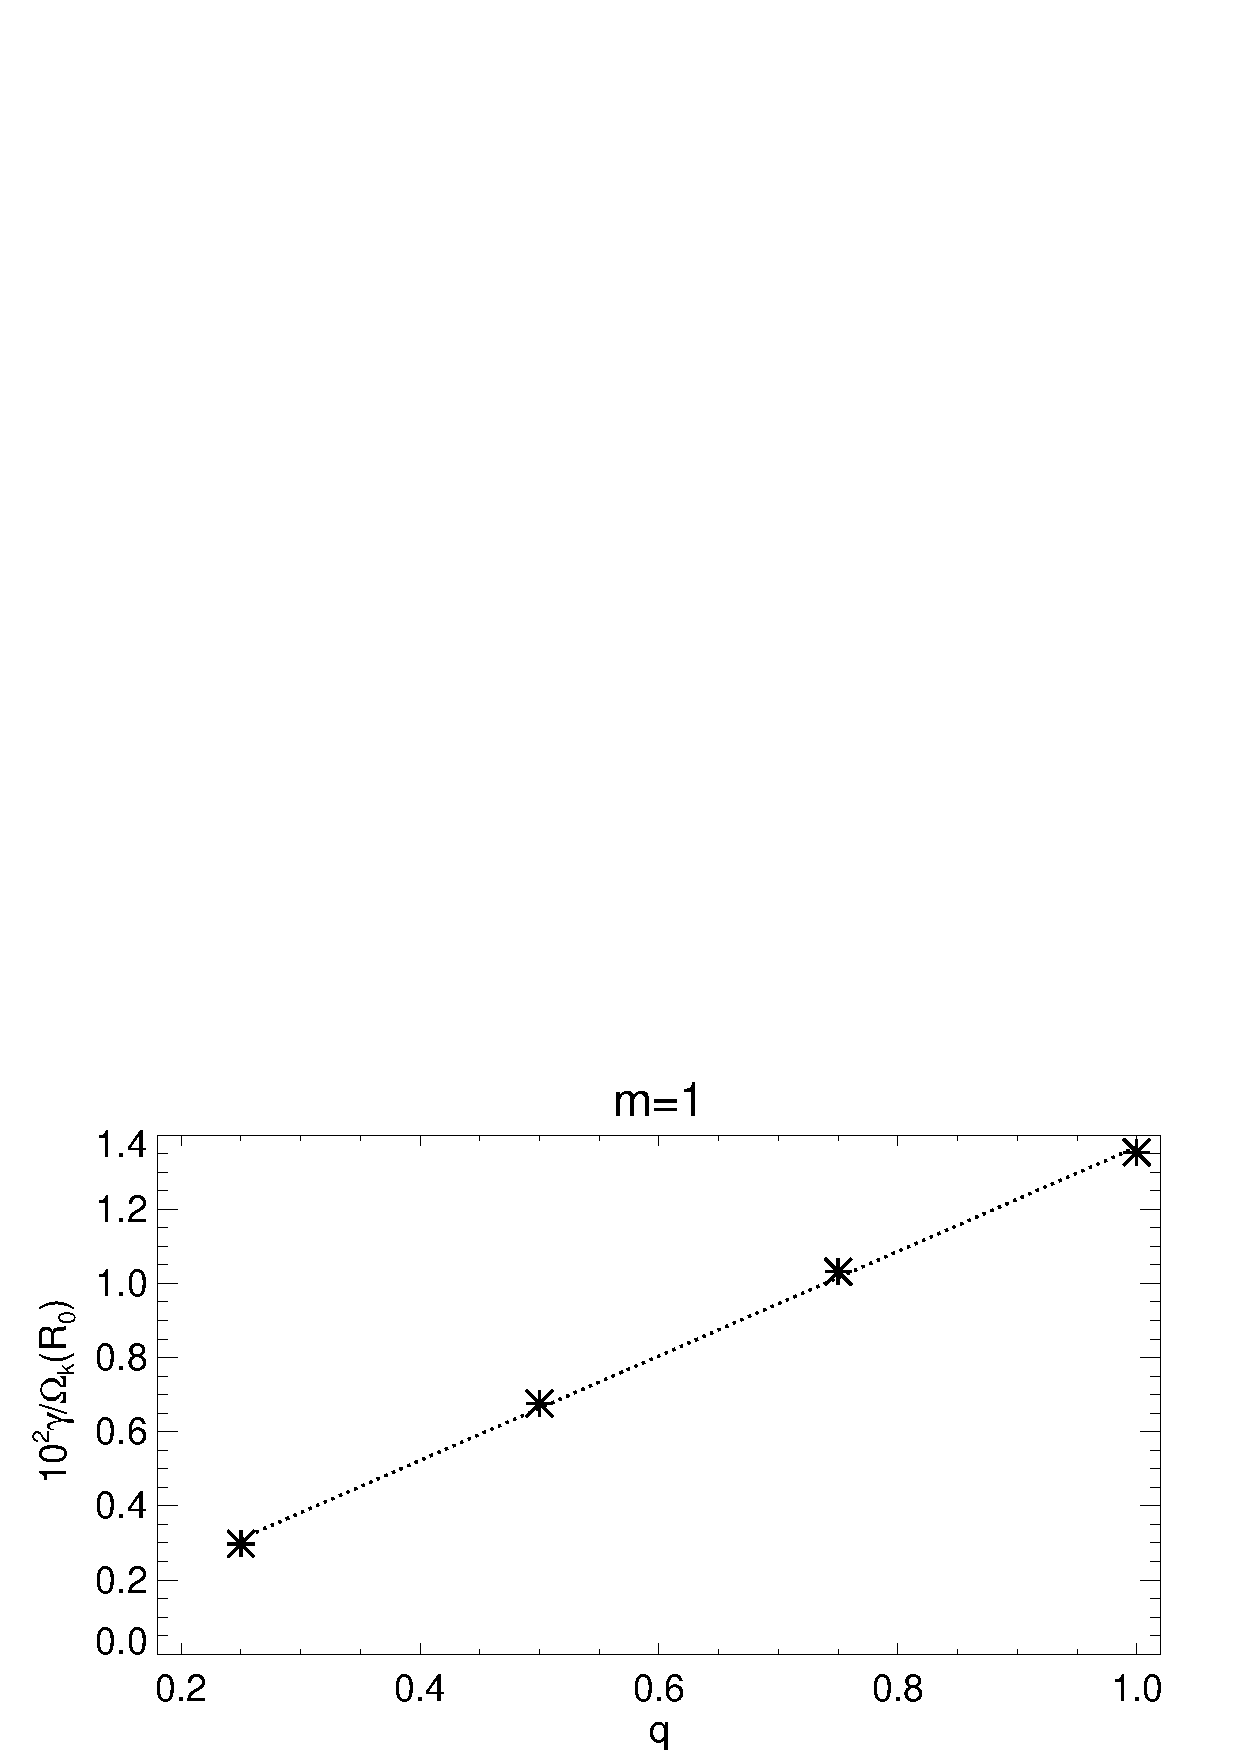
\includegraphics[width=\linewidth]{figures/m1_analysis_plot_ratemax_fargo_varq}    
  \caption{Growth rates of the $m=1$ spiral mode as a function of the
    imposed sound-speed gradient $q$ (asterisks). A linear fit is also 
    plotted (dotted line). 
    \label{fargo_varq_growth}} 
\end{figure}
%maybe extend the low q simulations to get better rates?

We also performed a series of simulations with variable aspect-ratio 
$h\in[0.03,0.07]$ but fixed $q=1$. This affects the magnitude of the temperature
gradient since $c_s \propto h$. However, with other parameters equal
to that in the fiducial simulation,  varying $h$ also changes the disc
mass. For $h\in[0.03,0.07]$ the total disc mass ranges from
$M_d=0.052M_*$ to $M_d=0.12M_*$ and the 
mass within $R\in[R_1,R_2]$  ranges from $0.033M_*$ to $0.062M_*$. 
% similar Q profiles

Fig. \ref{fargo_varh_growth} shows the growth rates of the $m=1$
spiral in $R\in[R_1,R_2]$ as a function of $h$. Growth rates increases
with $h$, roughly as  
\begin{align*}
  \gamma \simeq \left[0.10h + 8.3\times10^{-3}\right]\Omega_k(R_0).  
\end{align*}
However, a linear fit is less good than for variable $q$ cases above. This
may be due to the change in the total disc mass when $h$ changes. We
find no qualitative difference between the spiral pattern that
emerges. 

\begin{figure}
  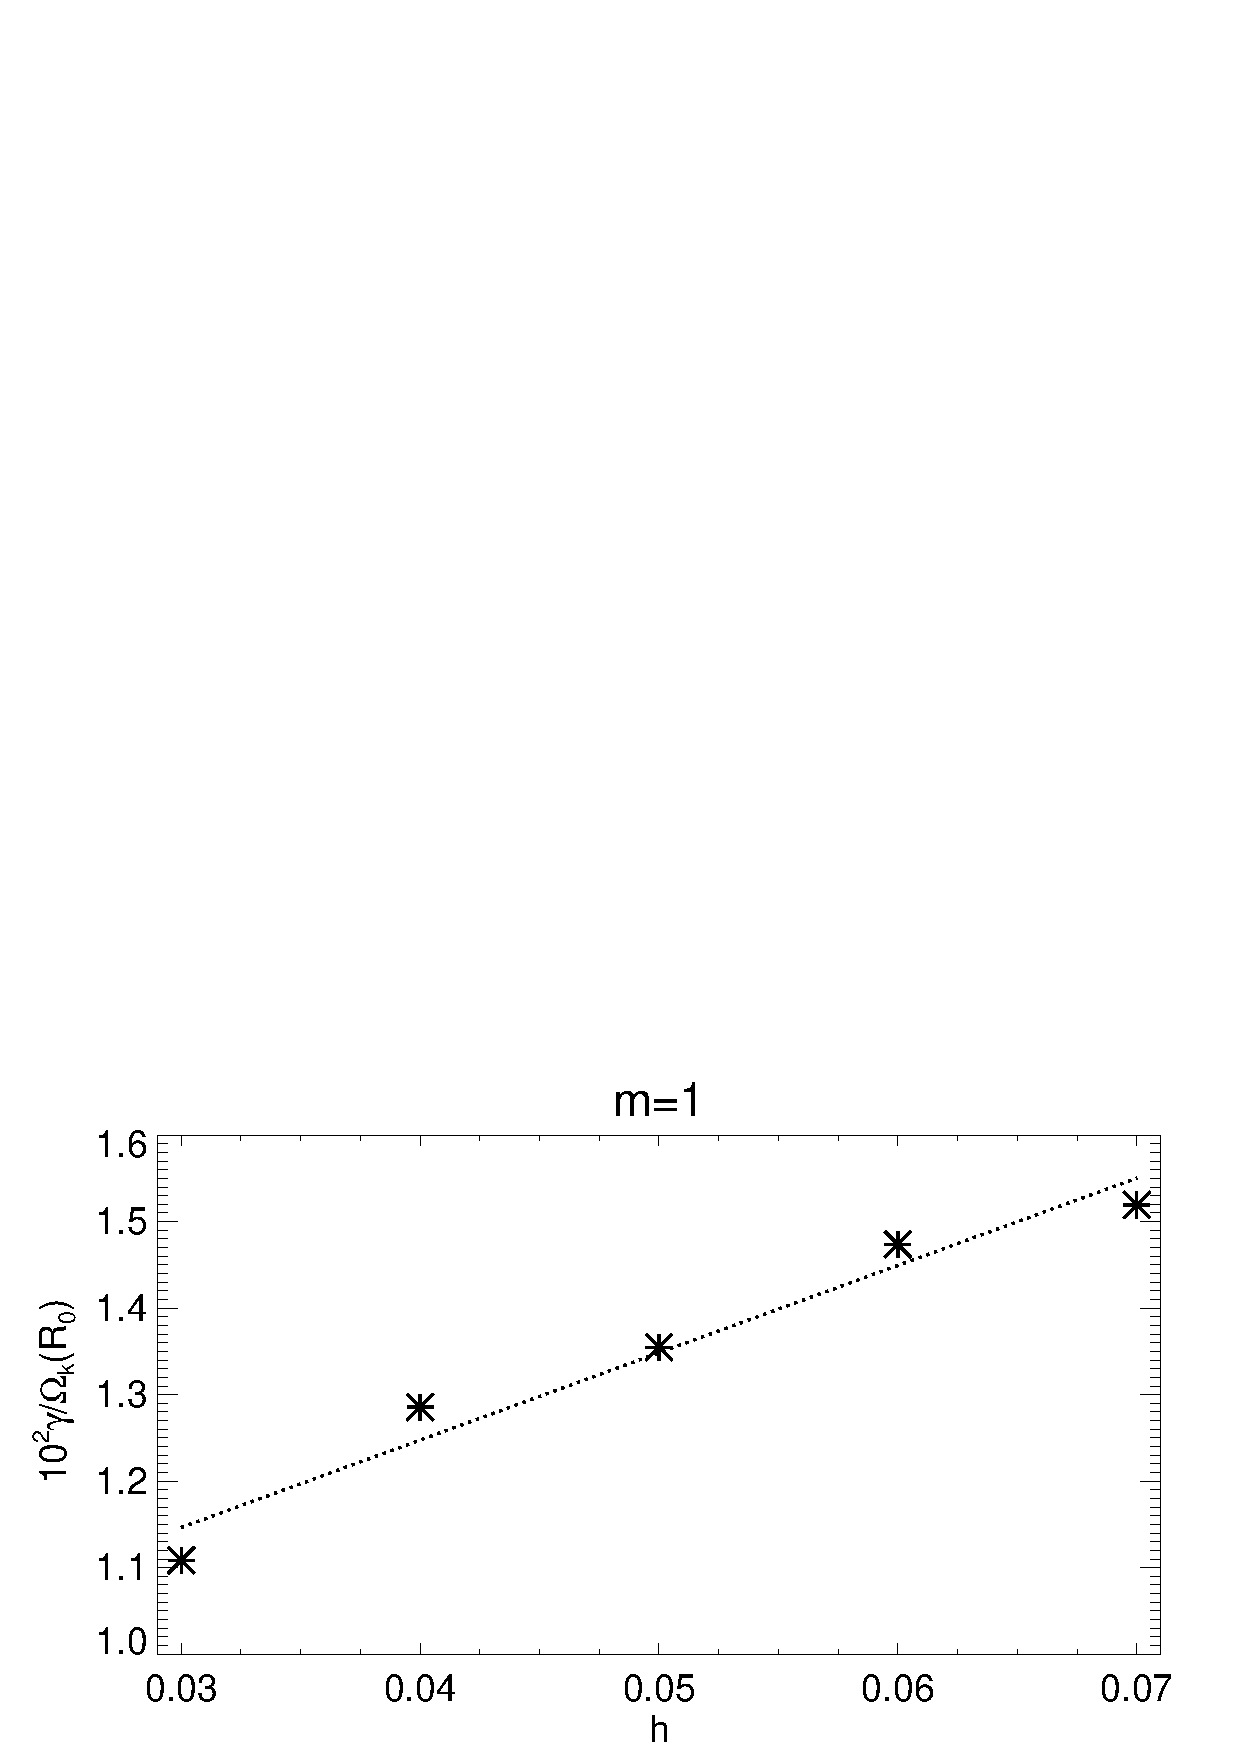
\includegraphics[width=\linewidth]{figures/m1_analysis_plot_ratemax_fargo_varh}    
  \caption{Growth rates of the $m=1$ spiral mode as a function of the
    disc aspect-ratio $h$ (asterisks). A linear fit is also
    plotted (dotted line). 
    \label{fargo_varh_growth}} 
\end{figure}

\section{Three-dimensional simulations}\label{results3d}
In this section we review 3D simulations carried 
out using ZEUS-MP and PLUTO. The main purpose is to verify 
the above results with different numerical codes, and validate  
the 2D approximation.    

The 3D disc has radial size
$[r_\mathrm{min},r_\mathrm{max}]=[0.4,10]R_0$ and vertical extent  
$n_H=2$ scale-heights at $R=R_0$. The resolution is $N_r\times N_\theta\times
N_\phi=256\times32\times512$, or about $4$ cells per
$H$. Because of the reduced resolution 
compared to 2D, we use a smooth perturbation by setting
$\delta = 10^{-3}$ and $M=1$ in Eq. \ref{randpert}. This corresponds
to a single $m=1$ disturbance in $R\in[R_1,R_2]$.
%, which
%eventually dominates in 2D simulations.  

The 3D discs are initialised in approximate equilibrium only, so we
first evolve the disc without perturbations using  
$(\lmax,\mmax)=(32,0)$ up to $t=10P_0$, during which 
meridional velocities are damped out. We then restart the simulation
with the above perturbation and $(\lmax,\mmax)=(32,32)$, and damp
meridional velocities near the radial boundaries. 

Fig. \ref{3d_ampmax} plots the evolution of the $m=1$ spiral amplitudes measured
in the ZEUS-MP and PLUTO runs. We also ran simulations
with a strictly isothermal equation of state ($q=0$), which display no
growth compared to that with a temperature gradient.  This confirms
the temperature gradient effect is the same in 3D. 
%why no high m
                                %modes as in 2D for iso disc?
                                %resolution? 

In the ZEUS-MP run, we observed high-$m$ disturbances developed near 
the inner boundary initially, which is likely responsible for the
growth seen at $t<50P_0$. This is a numerical artifact and effectively
seeds the simulation with a larger perturbation. Results
from ZEUS-MP are therefore off-set from PLUTO by $\sim50P_0$. However,
once the coherent $m=1$ spiral begins to grow ($t\gtrsim 100P_0$), 
we measure similar growth rates in both codes: 
\begin{align*}
  &\gamma \simeq 0.0073\Omega_k(R_0) \quad\quad \mathrm{PLUTO},\\
  &\gamma \simeq 0.0085\Omega_k(R_0) \quad\quad \varA{ZEUS-MP}.
\end{align*}
Both are smaller than the 2D simulations, because of the 
lower resolutions adopted in 3D and/or the small softening length
employed in 2D. 
%Rc = 8.6R_0

\begin{figure}
  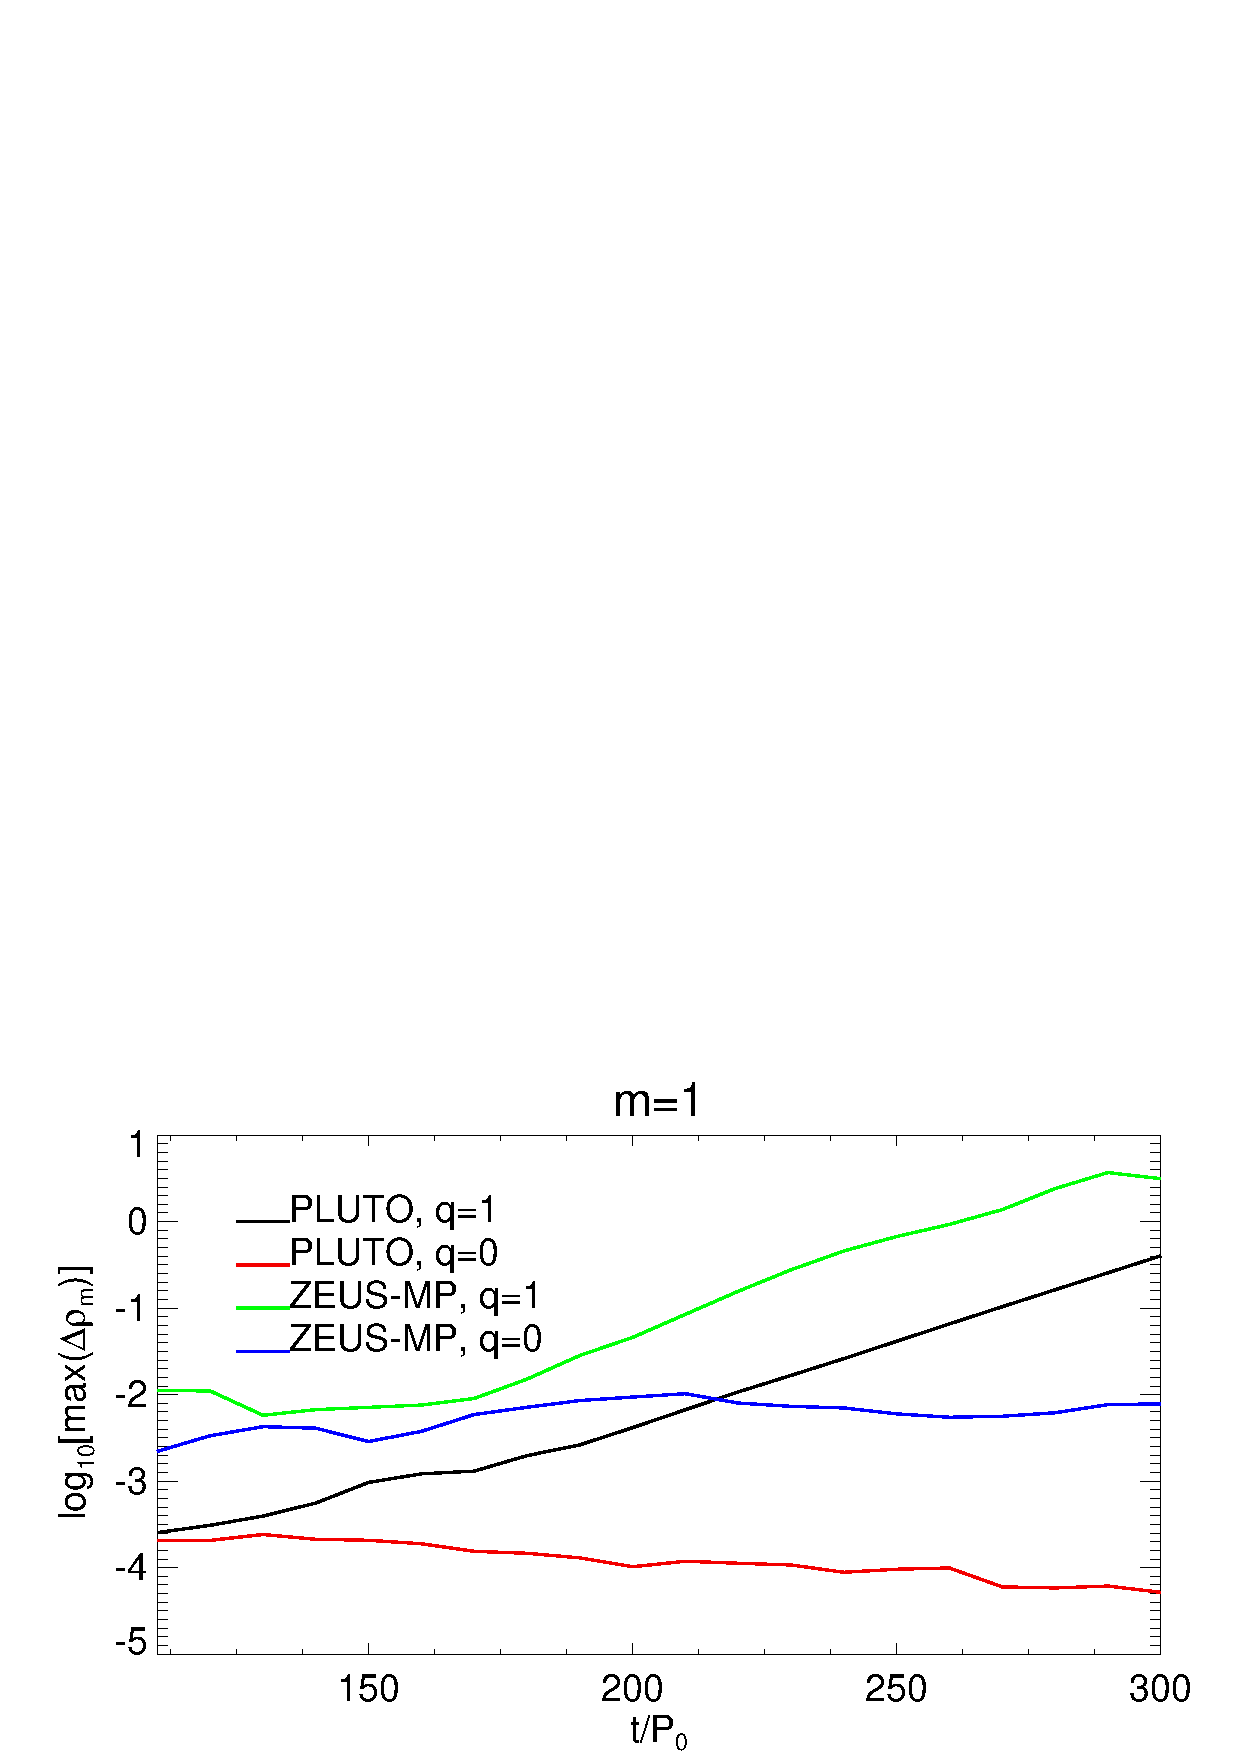
\includegraphics[width=\linewidth]{figures/m1_analysis_plot_ampmax3d}
  \caption{Evolution of the maximum $m=1$ density component in  $r\in[R_1,R_2]$
    in the 3D simulations. Results from discs with a 
    temperature gradient ($q=1$) and a strictly isothermal disc
    ($q=0$) are shown.  
    \label{3d_ampmax}}   
\end{figure}

%more global than 2D?

Visualisations of the 3D simulations are shown in   
Fig. \ref{3d_prelim} for the disc midplane and near the upper disc
boundary. The snapshots are chosen when the one-armed spirals in the two codes
have reached comparable amplitudes. %The agreement between the codes,
%as well as with the 2D simulations (Fig. \ref{2d_fargo_viz}), is
%satisfactory. 
Both codes show similar one-armed patterns at either height, and the
midplane snapshot is similar to the 2D simulation
(Fig. \ref{fargo_2d}). 
The largest spiral amplitude is found in the
self-gravitating region $R\in[R_1,R_2]$, independent of
height. However, notice the spiral pattern extends into 
the non-self-gravitating outer disc ($R>R_2$) at $z\sim 2H$, i.e.    
the disturbance becomes more global away from the midplane.  
%2d only adequate for self-gravitaing region 
\begin{figure}
  \begin{center}
    \subfigure[ZEUS-MP]{
      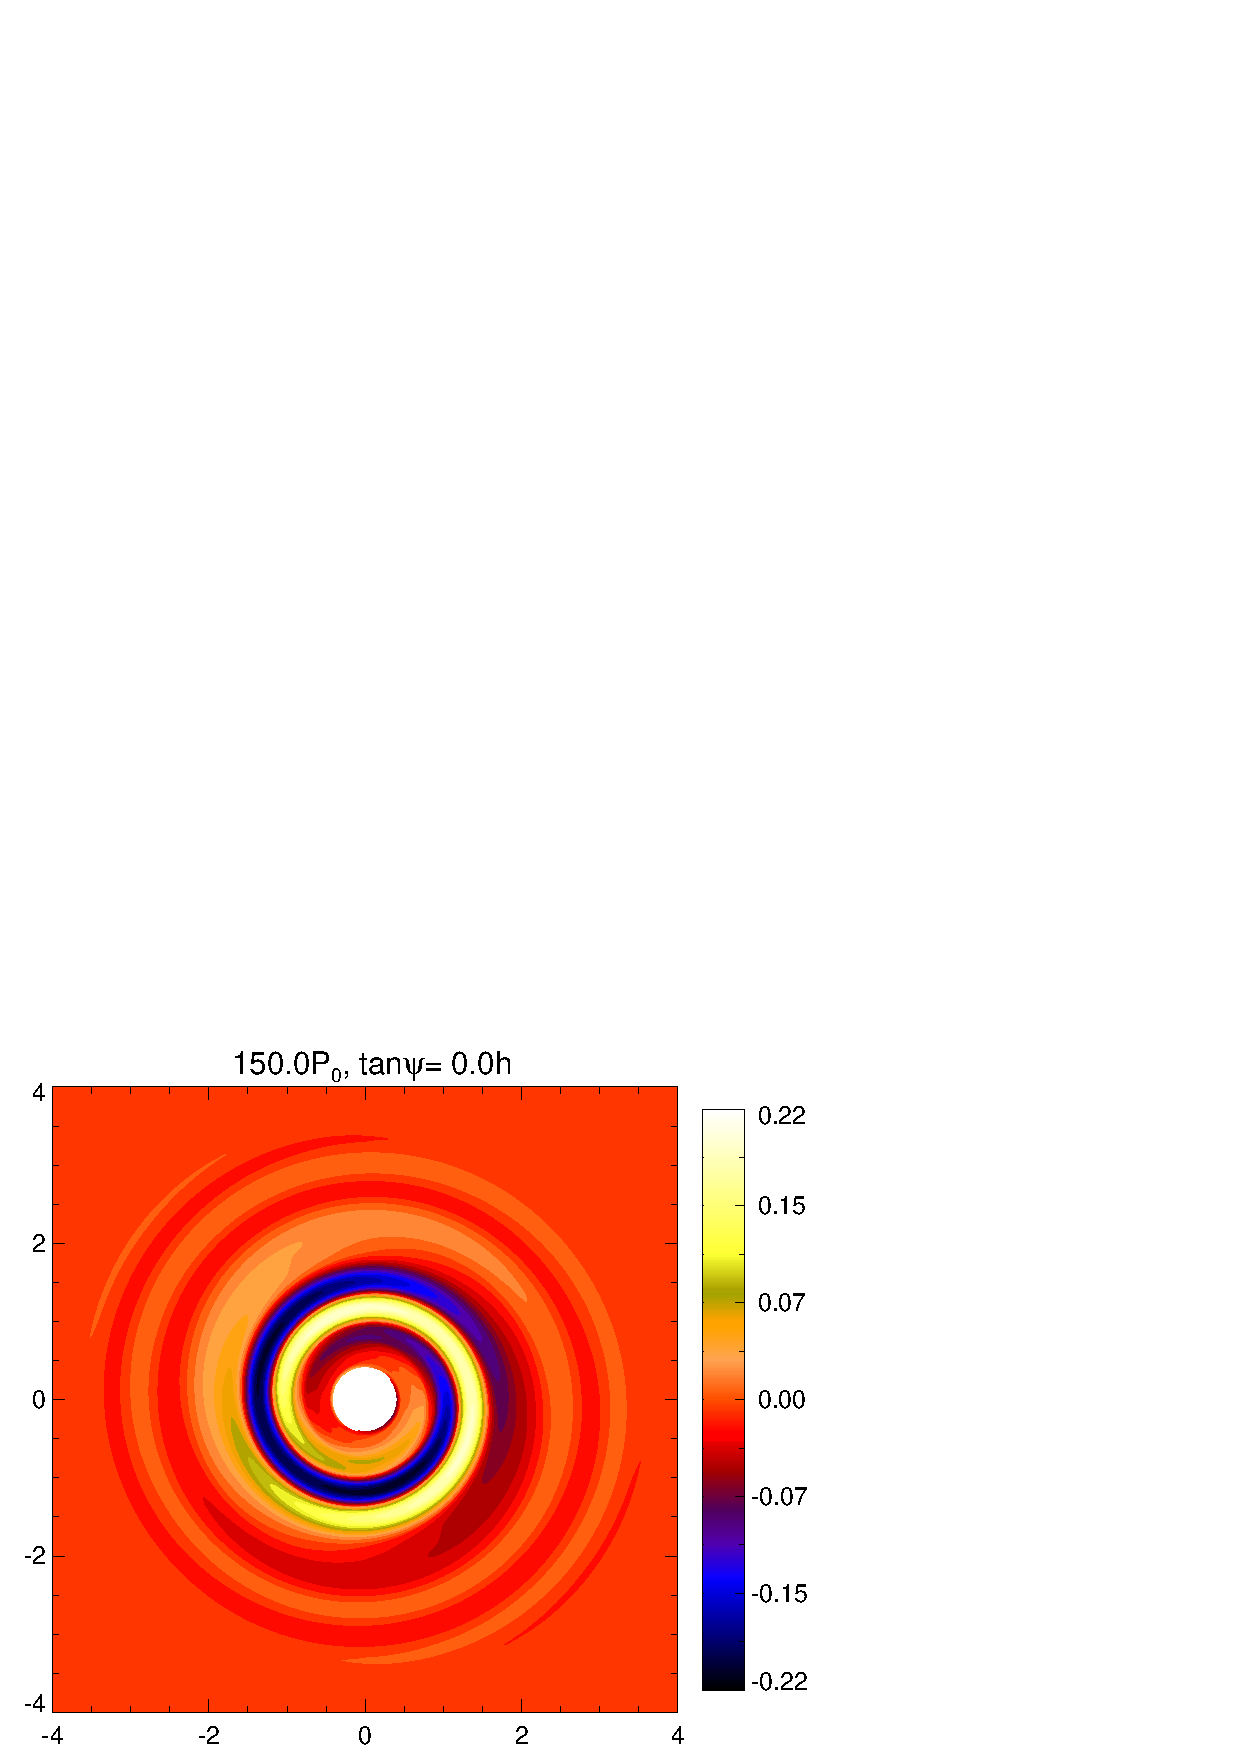
\includegraphics[scale=0.305,clip=true,trim=0cm 0cm 0cm 0cm]{figures/polarxy2_dens015_z0}  
      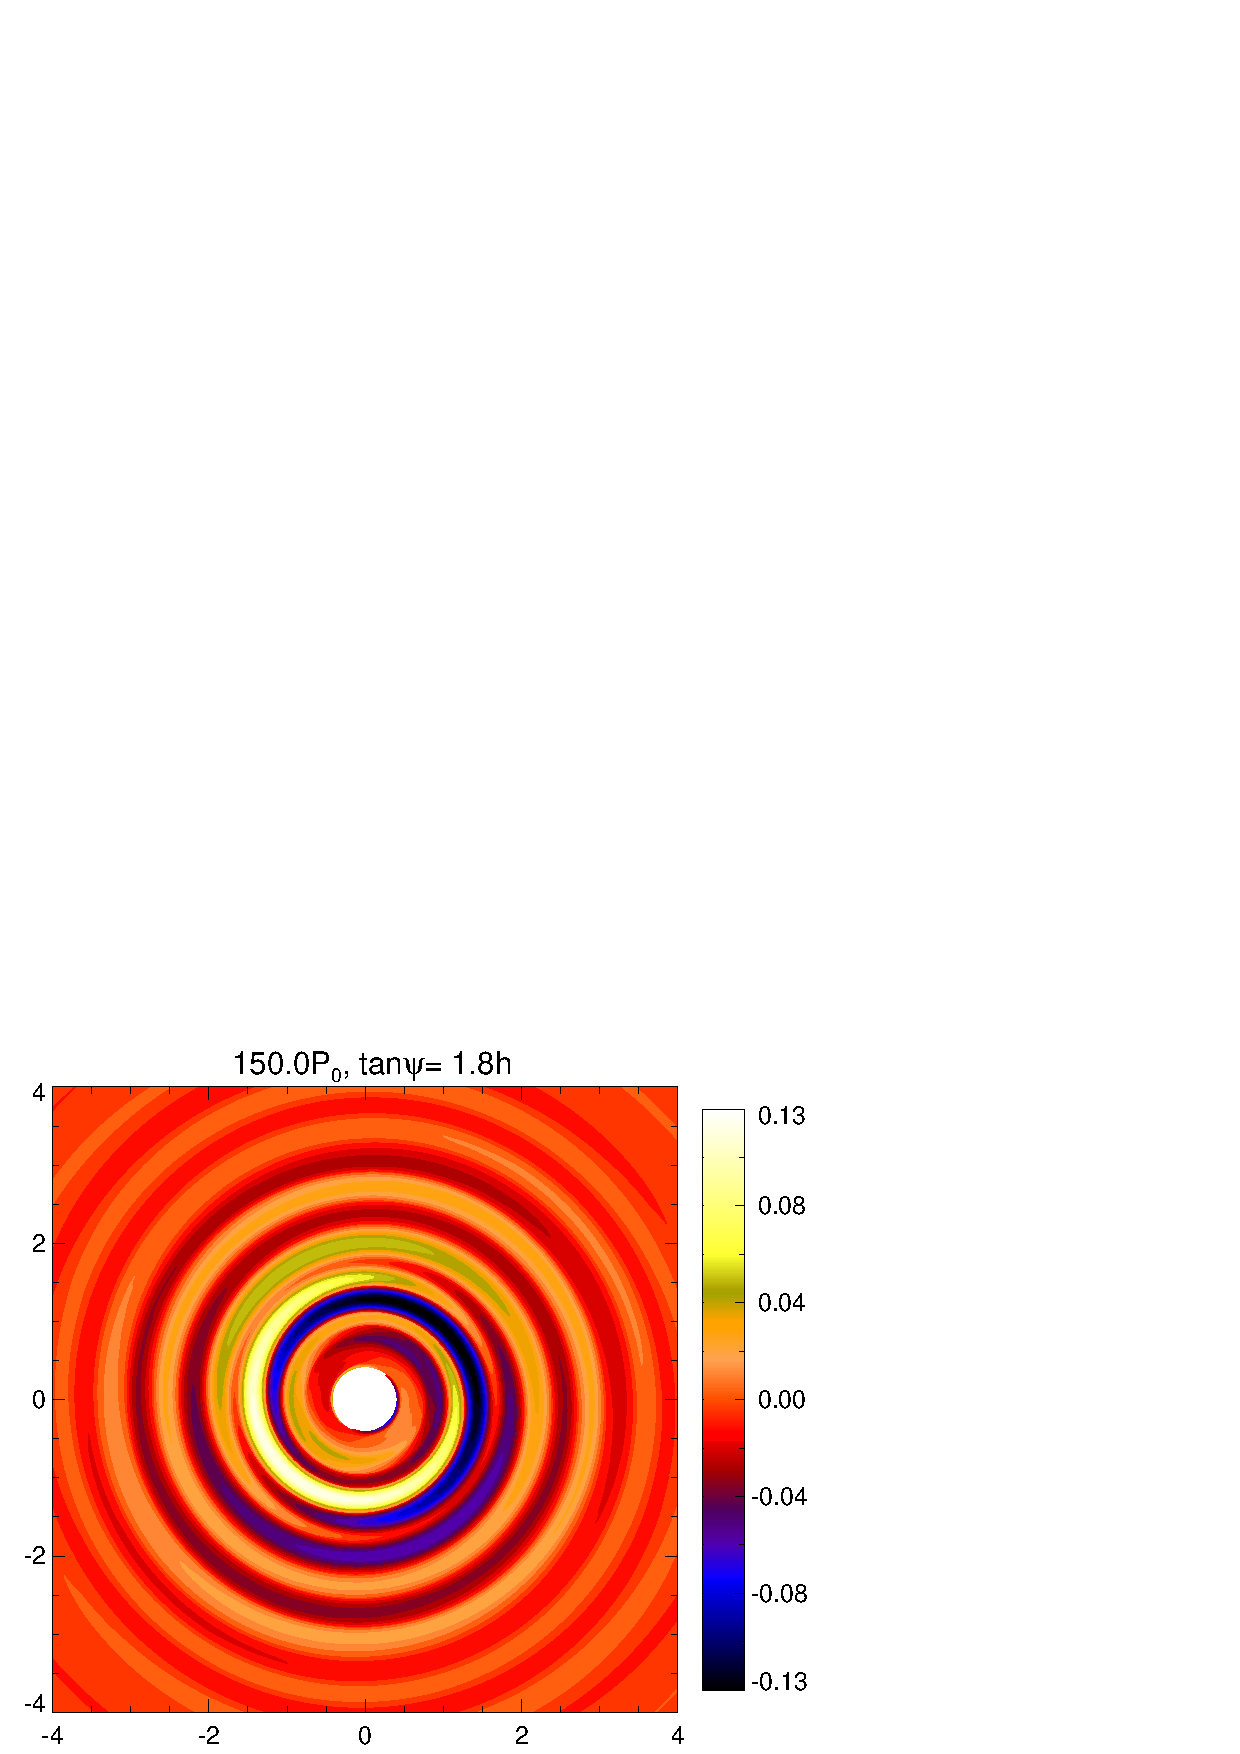
\includegraphics[scale=0.305,clip=true,trim=0.8cm 0cm 0cm
      0cm]{figures/polarxy2_dens015_zmax}  
    }
    \subfigure[PLUTO]{
      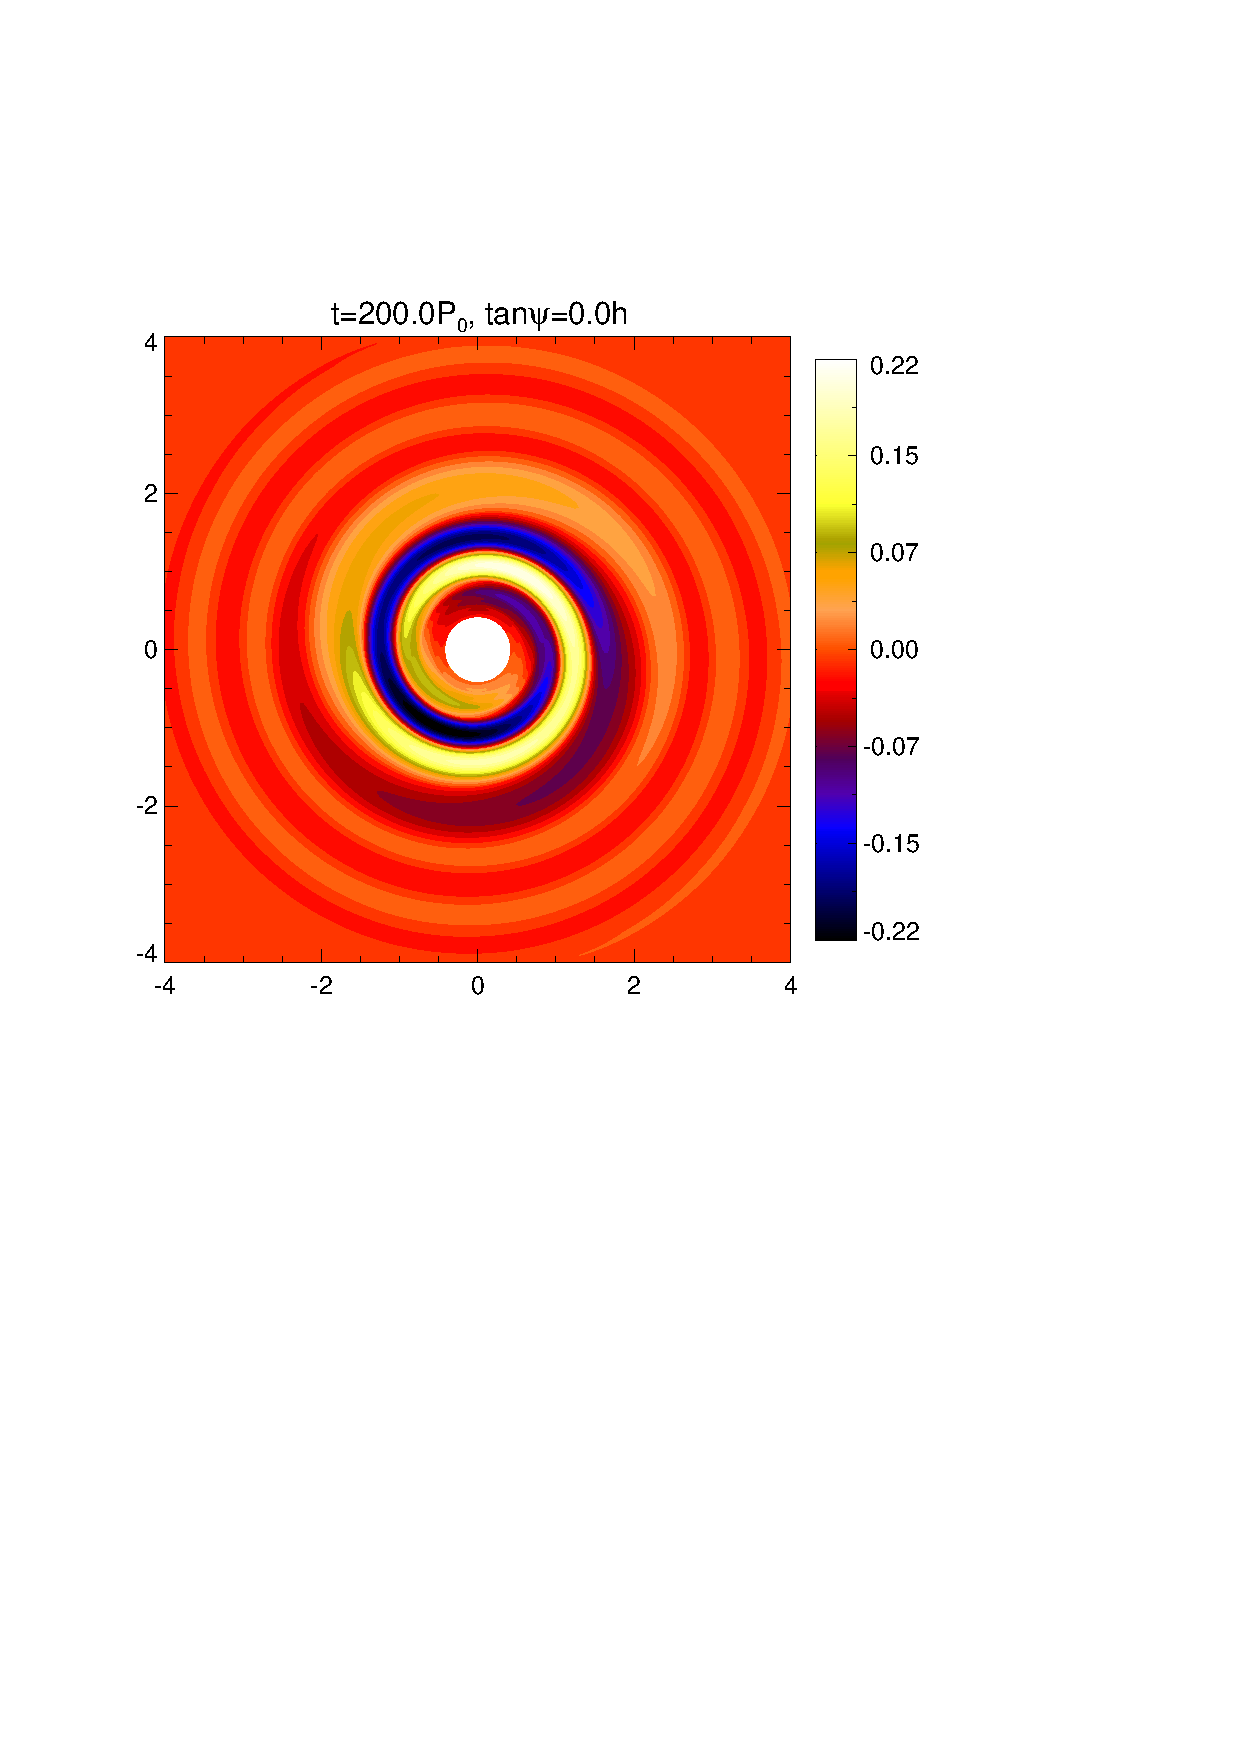
\includegraphics[scale=0.305,clip=true,trim=0cm 0cm 0cm 0cm]{figures/pdiskxy_023_z0}
      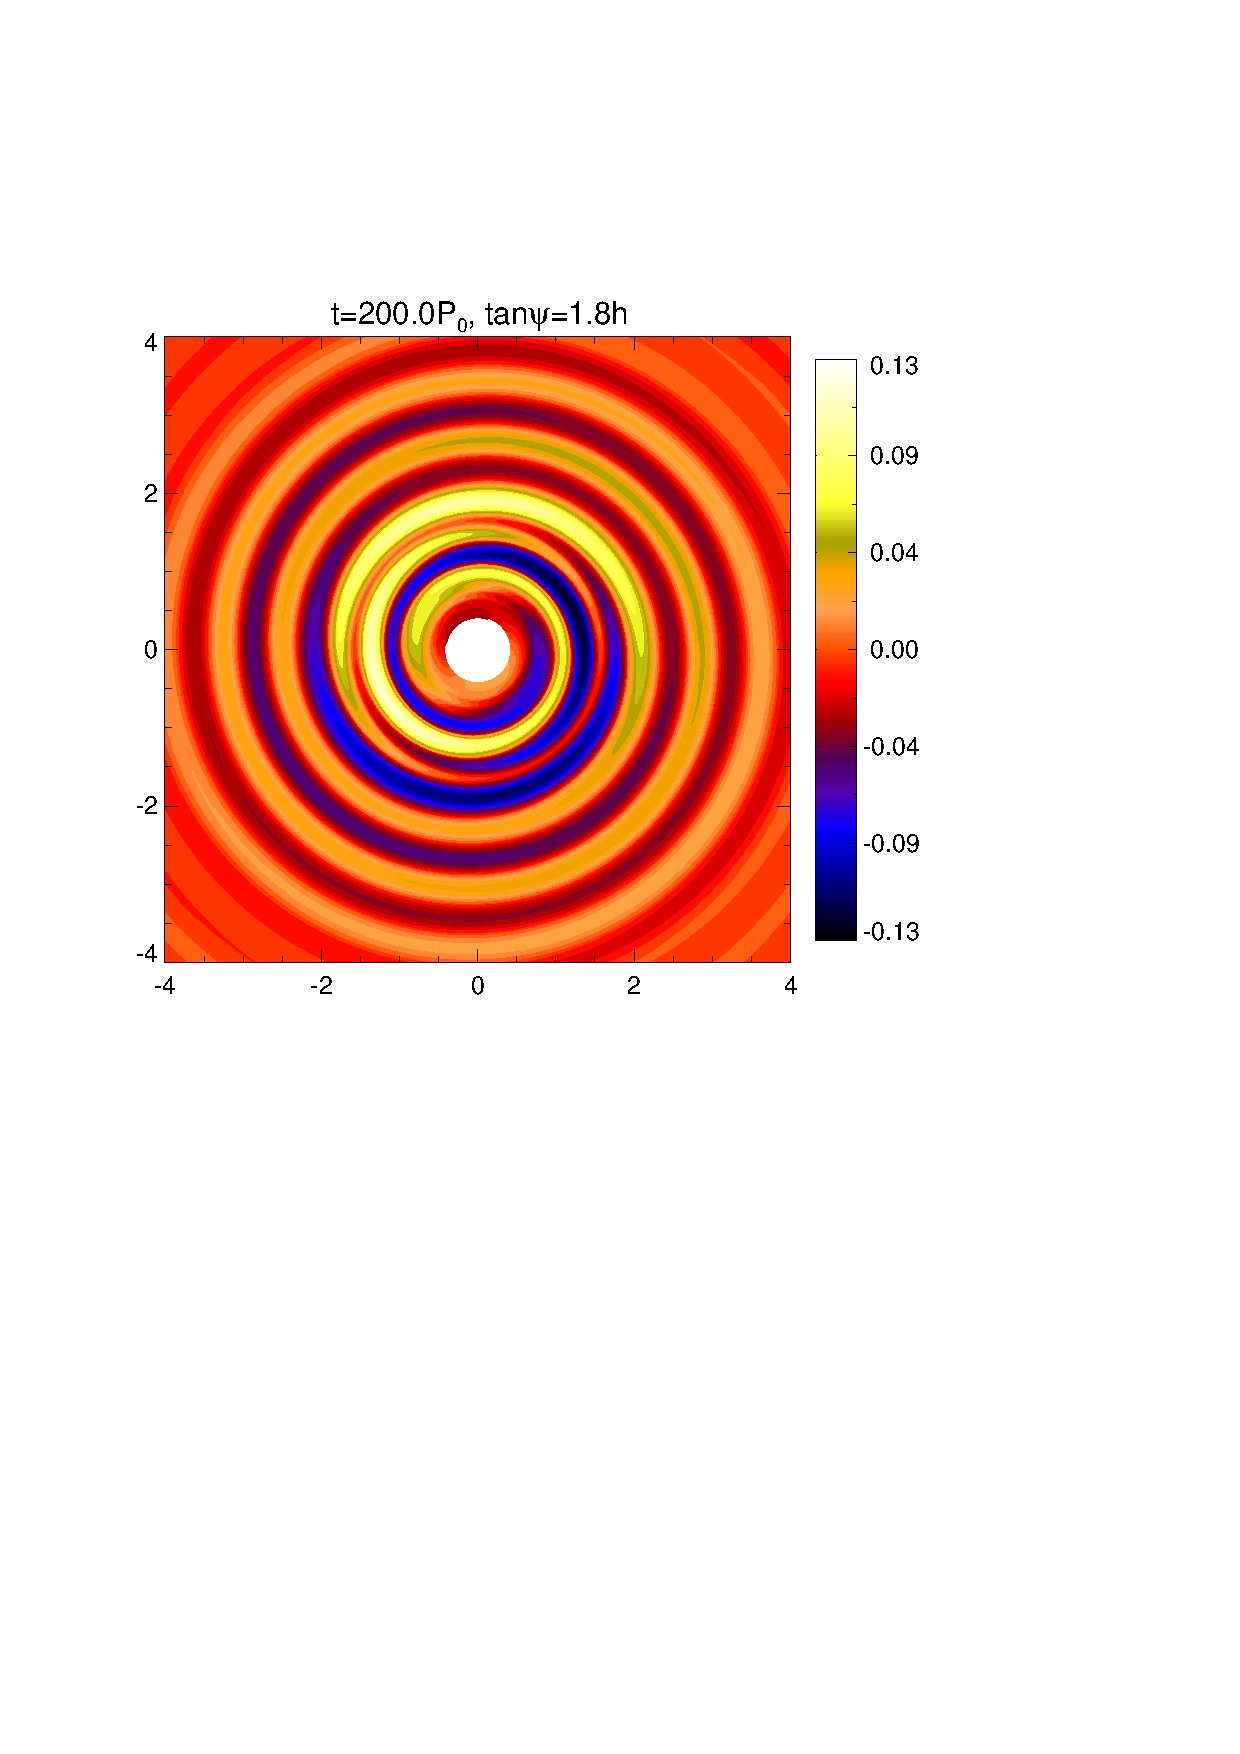
\includegraphics[scale=0.305,clip=true,trim=0.8cm 0cm 0cm
      0cm]{figures/pdiskxy_023_zmax}
    }
  \end{center}
  \caption{Three-dimensional simulations using the ZEUS-MP (top) and 
    PLUTO (bottom) codes. The $m=1$ density component $\Delta\rho_1$
    at the midplane (left) and approximately 
    two scale-heights above the midplane (right) is shown. Here $\psi
    \equiv \pi/2 - \theta$ is the angular height  
    from the midplane. \label{3d_prelim}}   
\end{figure}

\subsection{Vertical structure}
Fig. \ref{3d_rz} shows the vertical structure of the one-armed 
spiral in the PLUTO run. The spiral is vertically confined to $z
\lesssim H$ at $R\sim R_0$ (the self-gravitating region). Thus, a 2D
disc model, representing dynamics near the disc midplane, is  
sufficient capture the instability. However, for $R>2R_0$ the spiral amplitude
increases away from the midplane. It remains  
small in our disc model ($|\Delta\rho_1| \lesssim 0.1$), but could become 
significant with a larger vertical domain. This means that 3D 
simulations are necessary to study the effect of the one-armed spiral
on the exterior, non-self-gravitating disc.  
   
\begin{figure}
  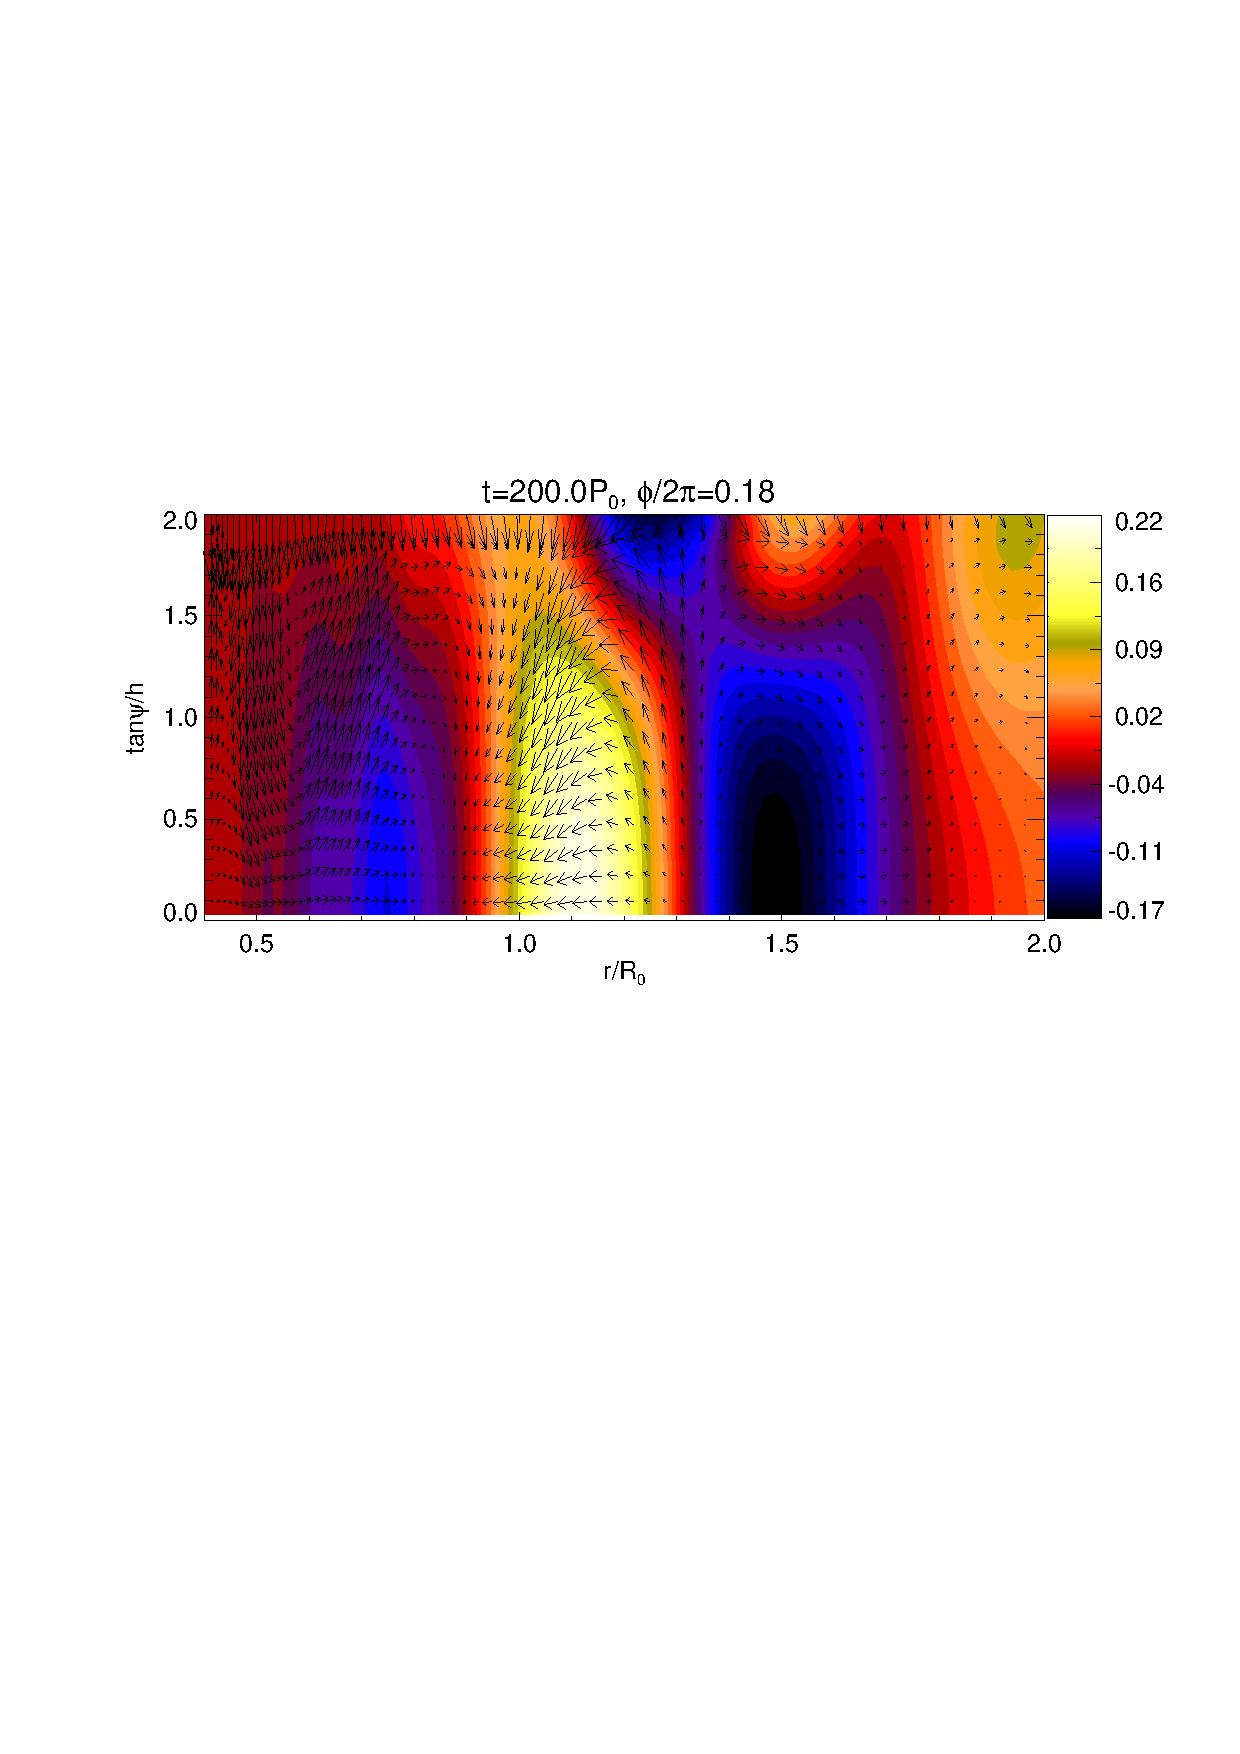
\includegraphics[scale=0.47,clip=true,trim=0cm 0.79cm 0cm
  0cm]{figures/pdisk_rz_023_sg}  
  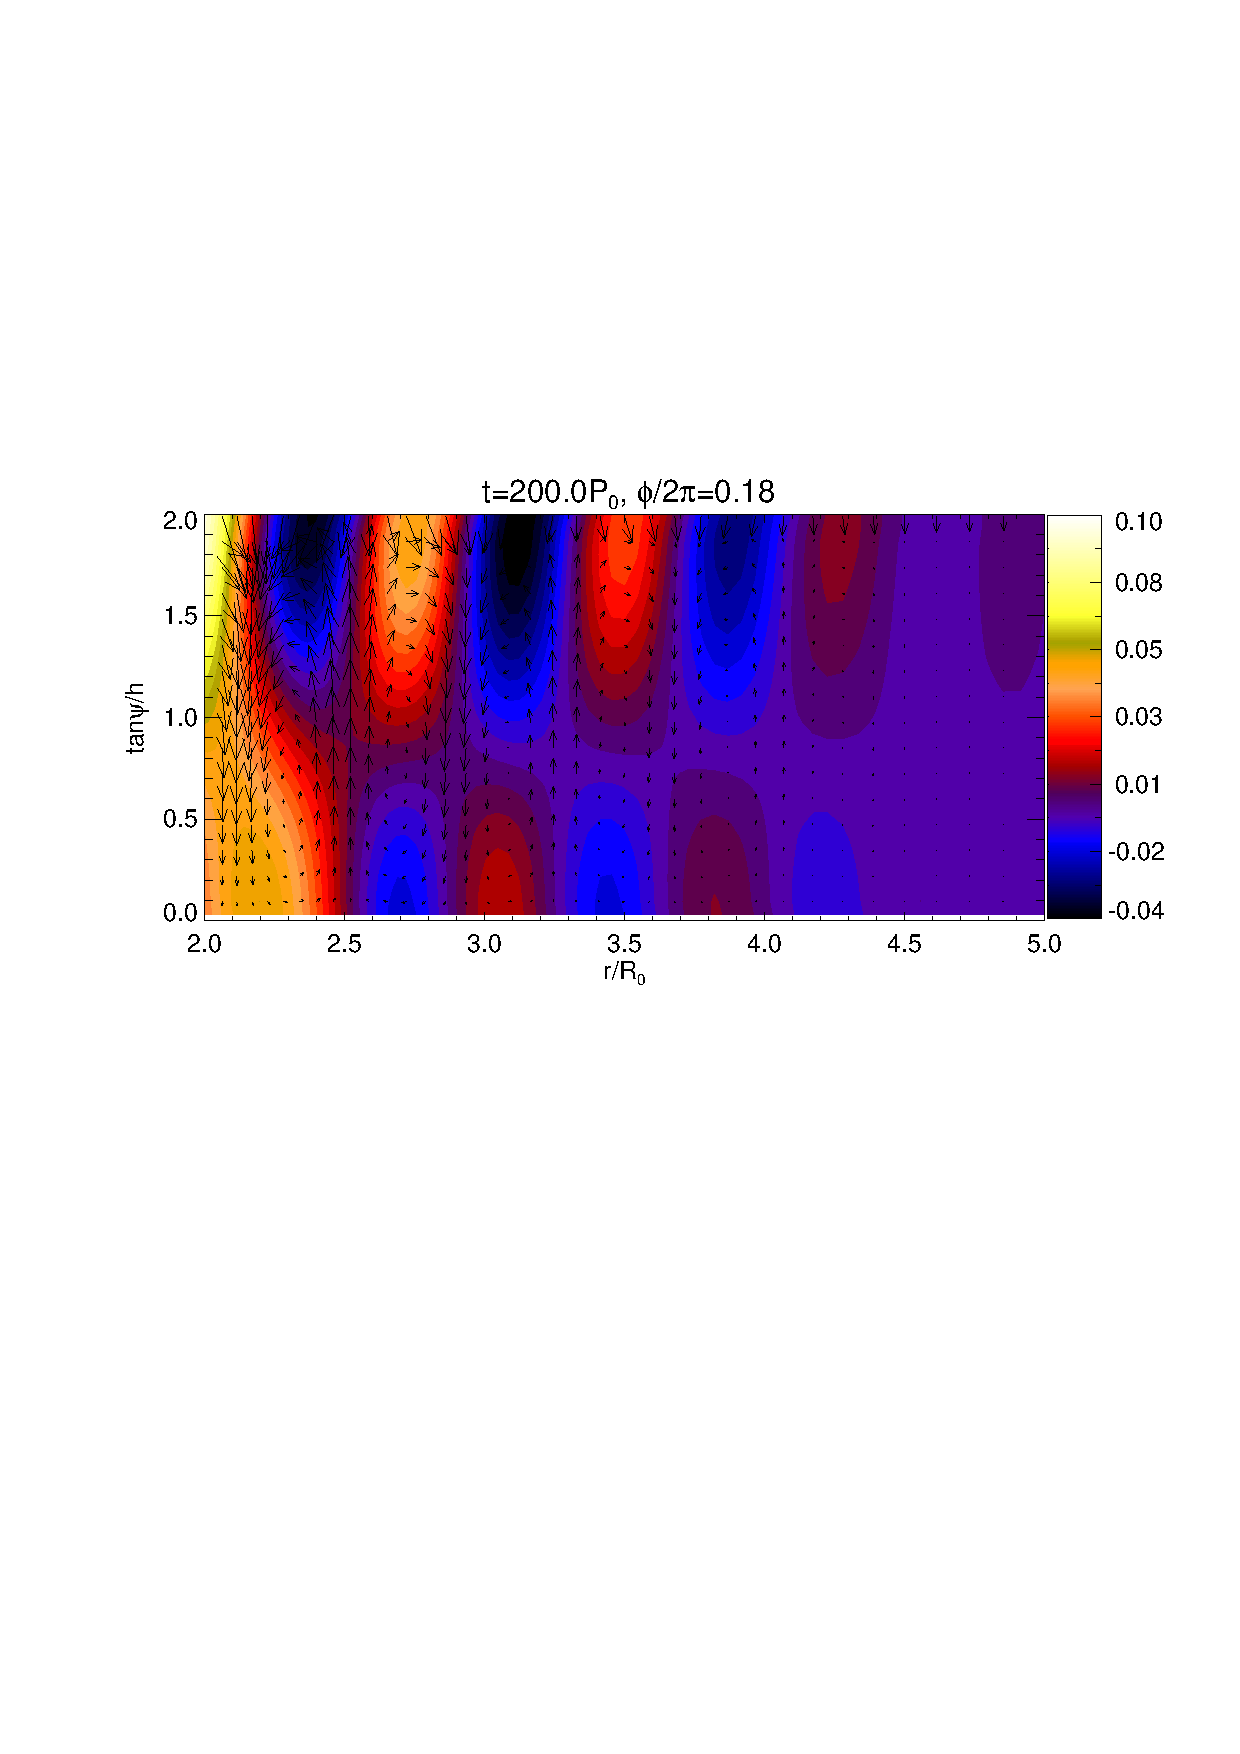
\includegraphics[scale=0.47,clip=true,trim=0cm 0cm 0cm
  0.64cm]{figures/pdisk_rz_023_nsg}  
  \caption{The $m=1$ density component in the meridional plane in the 
    PLUTO simulation. The slices are taken at the azimuth of   
    $\mathrm{max}[\Delta\rho_1(r,\pi/2,\phi)]$. Arrows represent the vector 
    $(v_r/R_0,-v_\theta/rh\sin^2{\theta})$. The top (bottom) panel corresponds
    to the inner (outer) portions of the disc. 
    \label{3d_rz}} 
\end{figure}   

Although Fig. \ref{3d_rz} appears to display significant vertical motion,
we measure the three-dimensionality parameter $\Theta < 10^{-2}$
(Eq. \ref{theta}), so vertical motions are insignificant compared to
horizontal motions. This supports a 2D approximation. On the other
hand, we find  $\mathrm{max}|v_z/c_s|\sim 0.2$ which, although
sub-sonic, is not very small.  
%may increase with height 

\subsection{Angular momentum conservation}   
Fig. \ref{3d_angmom} shows the angular momentum evolution in the 3D 
runs during the linear growth of the one-armed spiral. Because the
ZEUS-MP simulation is off-set from PLUTO, the time interval for the
plot was chosen such that the change in the angular momentum
components are comparable in the two codes. 

ZEUS-MP does not conserve angular momentum very well, but the
variation in total angular momentum $|\Delta J/J|< O(10^{-6})$ is
small compared to the individual components $|\Delta J_{0,1}/J|\sim
10^{-4}$. %it worsens with time 
PLUTO reaches similar values of $|\Delta J_{0,1}|$, but achieves better
conservation, with $|\Delta J/J|=O(10^{-8})$. These plots are again
similar to the 2D simulations, i.e. angular momentum lost by $J_1$ is
gained by $J_0$. This confirms that the interaction between $J_1$ and
$J_0$ operates in 3D and 2D similarly.  

\begin{figure}
%scale=0.41
  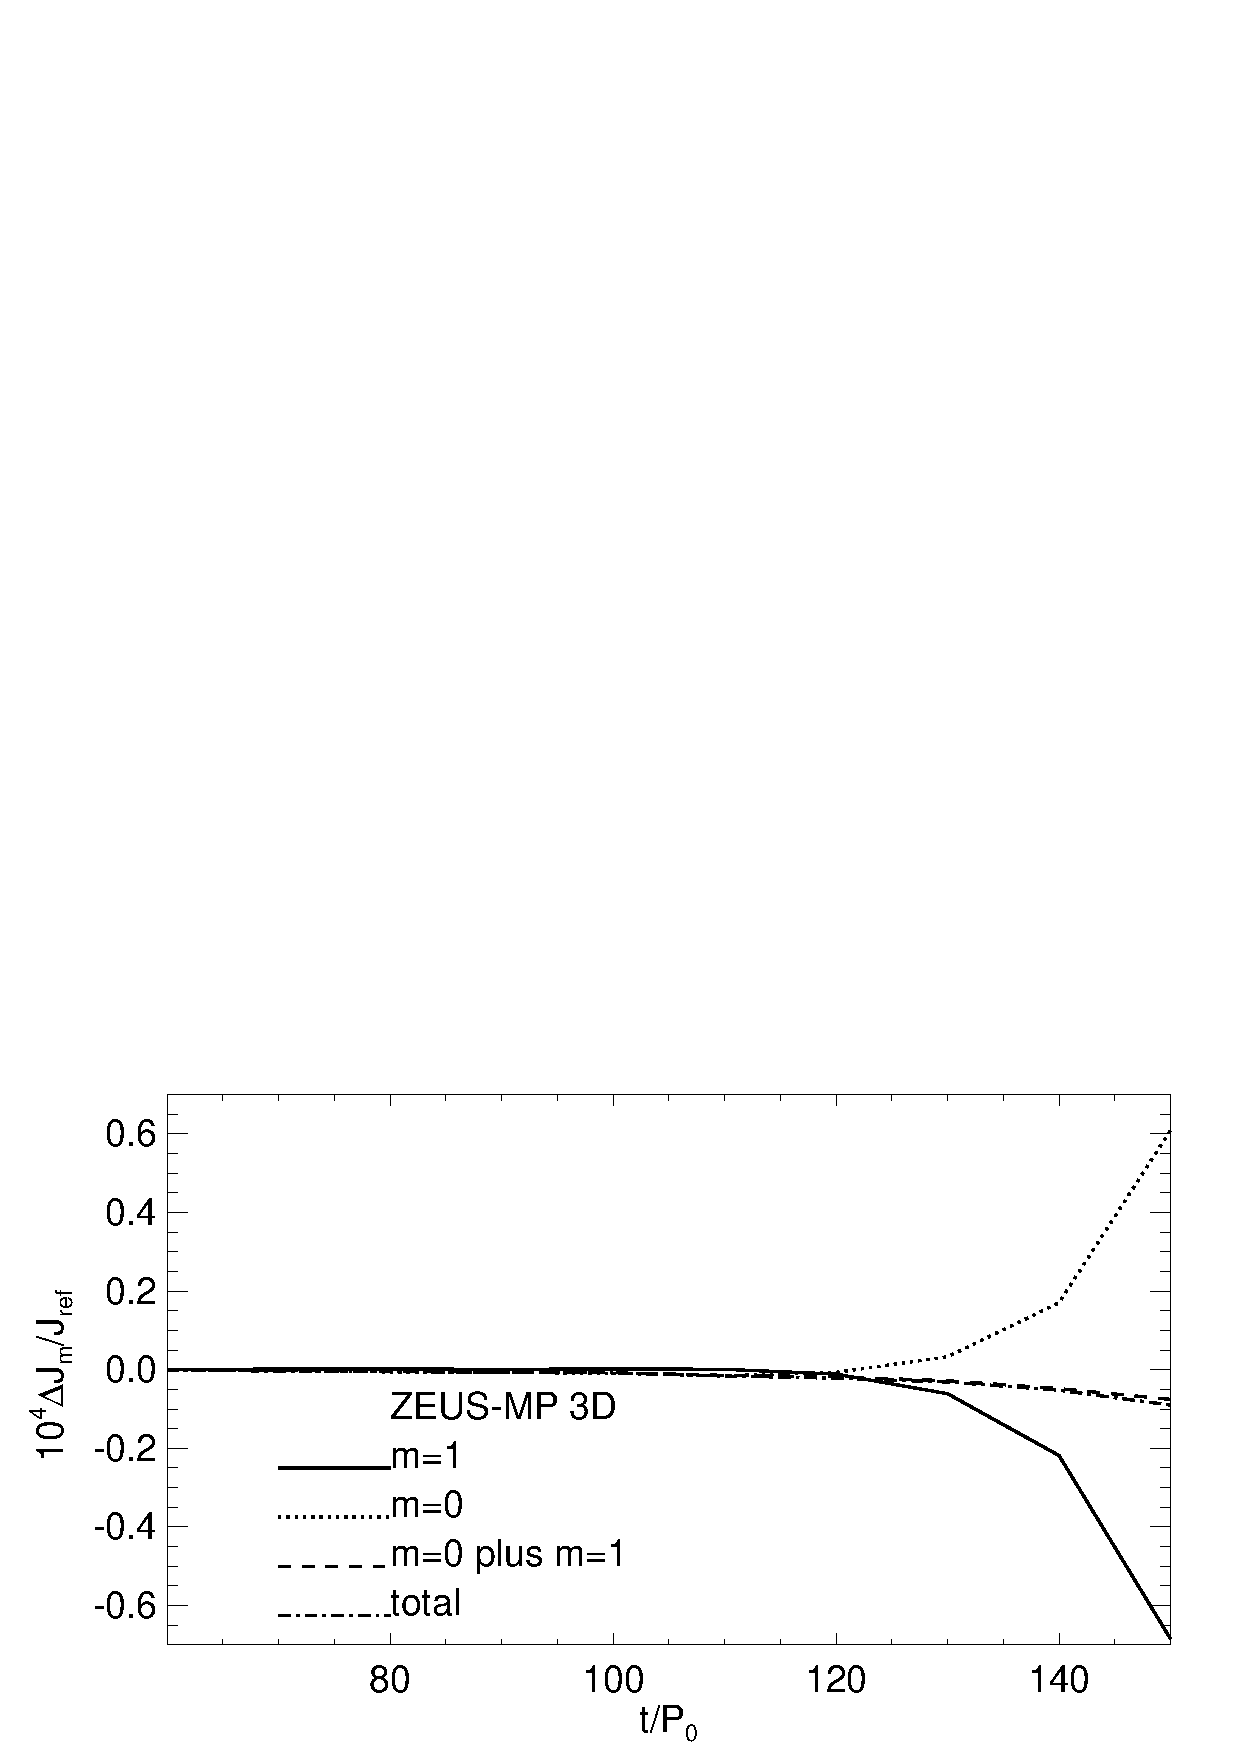
\includegraphics[scale=.41,clip=true,trim=0cm 1cm 0cm 0cm]{figures/nonaxi_evol_ang_zeus}
  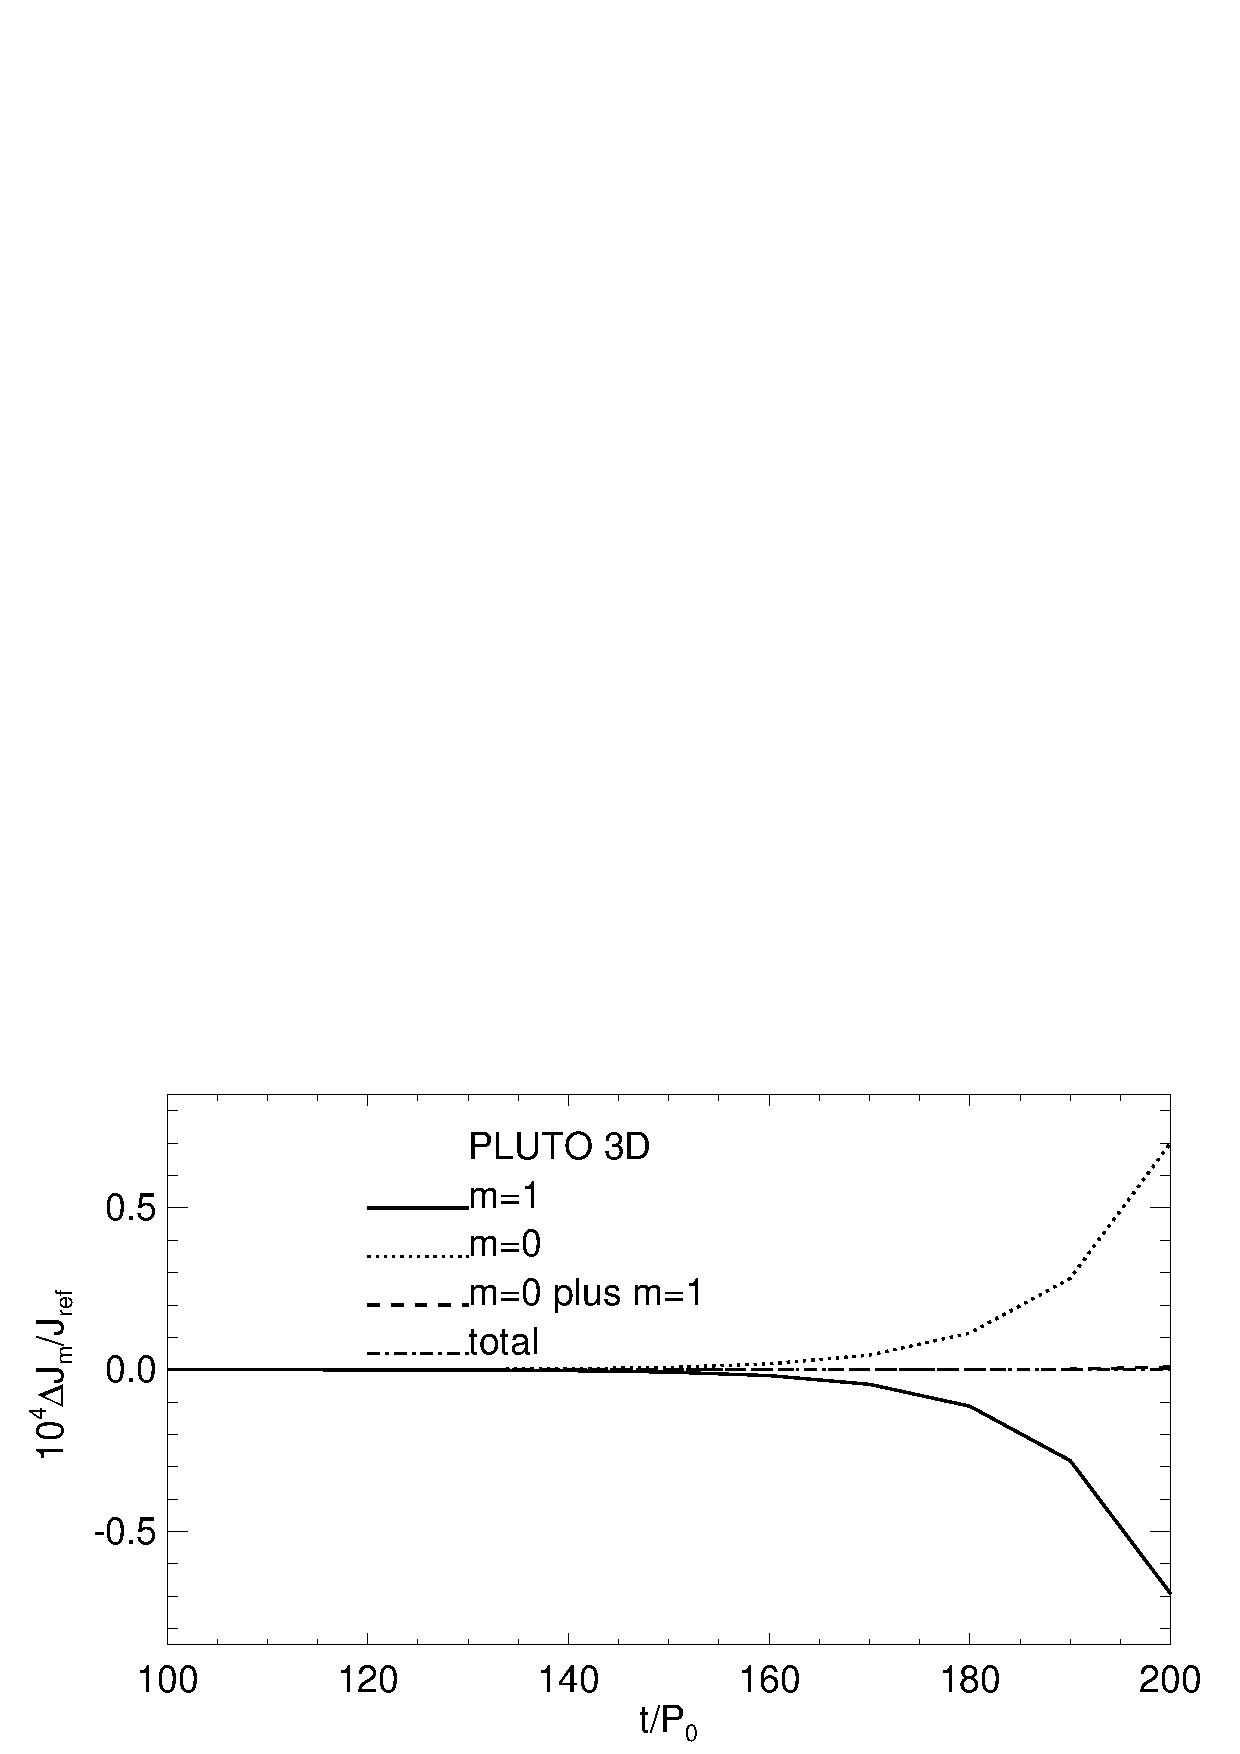
\includegraphics[scale=.41]{figures/nonaxi_evol_ang_pluto}
  \caption{Evolution of angular momentum components in the 3D 
    simulations. The perturbation 
    relative to $t=10P_0$, during the growth of the one-armed spiral,
    is shown in units of the initial total angular momentum
    $J_\mathrm{ref}$.\label{3d_angmom}}  
\end{figure}   


\section{Discussion}\label{discussions} 
Having confirmed the $m=1$ spiral instability through numerical
simulations, we now use results from the simulations combined with
linear theory to construct an explanation for their growth. For
simplicitly, we return to 2D discs. 


% According to previous studies \citep{adams89}, our disc models
% should not support $m=1$ linear spiral instabilities. This is because
% our discs are not sufficiently massive ($M_d\lesssim 0.1M_*$) and, more
% importantly, we have surpressed the motion of the central star. The 
% latter can induce $m=1$ instabilities in massive discs  \citep{shu90}.   


\subsection{Angular momentum density of  low-frequency $m=1$ modes}
From Eq. \ref{lin_ang_mom_cons} and assuming a time-dependence of the
form $\exp{(-\ii \sigma t)}$ with $\real{\sigma} = \omega$,  
the angular momentum density associated with linear waves is
\begin{align}
  \jlin = \frac{m\Sigma}{2}\left[\left(\omega -
      m\Omega\right)|\bm{\xi}|^2 + \ii\Omega\left(\xi_R\xi_\phi^* -
      \xi_R\xi_\phi^*\right)\right].  
\end{align}
For a low-frequency mode, $|\omega|\ll m\Omega$. Then neglecting the
term $\omega|\bm{\xi}|^2$ and setting $m=1$,
\begin{align}
  \jlin &\simeq \frac{\Sigma\Omega}{2}\left[-|\bm{\xi}|^2 + \ii\left(\xi_R\xi_\phi^* -
      \xi_R\xi_\phi^*\right)\right]\notag\\
  & = -\frac{\Sigma\Omega}{2}|\xi_R + \ii\xi_\phi|^2\notag\\
  & \leq 0.
\end{align}
Thus, low-frequency $m=1$ modes generally have negative
angular momentum. If the mode loses (positive) angular momentum
to the background, then we can expect instability. We demonstrate
this below. 

\subsection{Unstable interaction between low-frequency $m=1$ spirals
  and the background disc due to an imposed temperature gradient}
The $m=1$ spiral that emerges in our simulations have low frequency
($\Omega_p < \Omega$),
grows slowly ($\gamma\ll\Omega_p$), and its spatial form is consistent local theory  
(\S\ref{fargo_m1}). Then to a first approximation, we can regard it 
as a neutral, low-frequency $m=1$ mode in satifying the 
dispersion relation Eq. \ref{dispersion} in local theory.  %attribute
                                %growth to temp gradient 
To demonstrate possible instability, %we 
% first construct a neutral low-frequency mode using local theory, 
we show that the torque density acting on such a mode due to the background
temperature gradient is negative, which enforces the mode, because it
has negative angular mometum.  
% Note that
% we will not be assuming a self-gravitating disc until the end of this
% section. 

We begin by recalling the expression for the torque density due to a
locally isothermal equation of state,
\begin{align*}
  T_\mathrm{BG} = - \frac{m}{2}\frac{dc_s^2}{dR}\imag\left(\delta\Sigma_m\xi_R^*\right).   
\end{align*}
The Eulerian surface density perturbation is given by
\begin{align}\label{den_pert}
  \delta\Sigma_m = -\nabla\cdot\left(\Sigma\bm{\xi}\right) 
  = -\frac{1}{R}\frac{d}{dR}\left(R\Sigma \xi_R\right) - \frac{\ii m}{R}\Sigma\xi_\phi.  
\end{align}
We now invoke local theory by setting $d/dR \to \ii k$ where $k$ is
real, and assume $|kR|\gg m$ so that the second term on the right hand
side of Eq. \ref{den_pert} is negligible. Then    
\begin{align}
  \delta\Sigma _m  \simeq -\ii k \Sigma \xi_R,
\end{align}
which gives
\begin{align}
  T_\mathrm{BG} = \frac{m}{2}\frac{dc_s^2}{dR}k\Sigma |\xi_R|^2. 
\end{align}
% \begin{align}
%   T_\mathrm{BG} &= -\frac{m}{2}\frac{dc_s^2}{dR}\imag\left[\delta\Sigma_m \left(\frac{\delta
%         v_{Rm}}{-\ii\sbar}\right)^*\right] \notag\\
%   & = \frac{m}{2}\frac{dc_s^2}{dR}\imag\left[\ii \delta\Sigma_m \left(\frac{\delta
%         v_{Rm}}{\sbar}\right)^*\right]
% \end{align}
% where we replaced the radial Lagrangian displacement by the Eulerian
% radial velocity perturbation in Eq. \ref{baroclinic_torque}. 
% The linearised momentum equations give
% \begin{align}
%   D\delta v_{Rm} =& 
%   \ii\sbar\left[c_s^2\frac{d}{dR}\left(\frac{\delta\Sigma_m}{\Sigma}\right)
%     + \frac{d}{dR}\delta\Phi_m\right] \notag\\ 
%   &- \frac{2\ii
%     m\Omega}{R}\left(c_s^2\frac{\delta\Sigma_m}{\Sigma} +
%     \delta\Phi_m\right),
% \end{align}
% where $D\equiv \kappa^2 - \sbar^2$. 
% We now invoke local theory by setting $d/dR \to \ii k$ where $k$ is
% real, and using the local solution to the Poisson equation
% \begin{align}
%   \delta\Phi_m = -\frac{2\pi G}{|k|}\delta\Sigma_m 
% \end{align}
% \citep{shu91}. Then the radial velocity perturbation becomes
% \begin{align}
%   \delta v_{Rm} =
%   \frac{1}{D}\frac{\delta\Sigma_m}{\Sigma}\left(\frac{2\pi G
%       \Sigma}{|k|} - c_s^2\right)\left(k\sbar + \frac{2\ii
%       m\Omega}{R}\right),
% \end{align}
% so that 
% \begin{align}
%   \ii\delta\Sigma_m \left(\frac{\delta v_{Rm}}{\sbar}\right)^* =
%   \frac{1}{D^*}\frac{|\delta\Sigma_m|^2}{\Sigma}\left(\frac{2\pi G
%       \Sigma}{|k|} - c_s^2\right)\left(\ii k  + \frac{2
%       m\Omega}{R\sbar^*}\right). 
% \end{align}
% For a neutral mode, $\sbar$, and therefore $D$ is real. Then, after
% taking the imaginary part of the above expression, the torque
% density is 
% \begin{align}\label{tbg_explicit}
%   T_\mathrm{BG} &=
%   \frac{m}{2}\frac{dc_s^2}{dR}\left[\frac{k}{D}\frac{|\delta\Sigma_m|^2}{\Sigma}\left(\frac{2\pi G
%       \Sigma}{|k|} - c_s^2\right)\right].
% % &\simeq \frac{m}{2}\frac{dc_s^2}{dR}\left[\frac{k}{\left(\kappa^2 -
% %         m^2\Omega^2\right)}\frac{|\delta\Sigma_m|^2}{\Sigma}\left(\frac{2\pi
% %       G \Sigma}{|k|} - c_s^2\right)\right]. 
% \end{align}
% We now use the local dispersion relation,
% Eq. \ref{dispersion}, to make the replacement $D = 2\pi G \Sigma |k| -
% k^2c_s^2$ in the above expression. This gives
% \begin{align}\label{tbg_simple}
%   T_\mathrm{BG} =
%   \frac{m}{2}\frac{dc_s^2}{dR}\frac{1}{k}\frac{|\delta\Sigma_m|^2}{\Sigma}.  
% \end{align}  
This torque density is negative for trailing waves in discs with
a fixed temperature profile decreasing outwards ($k>0$ and $dc_s^2/dR<0$,
respectively). Note that this conclusion does not rely on the
low-frequency approximation and holds for any $m$.   

However, if the linear disturbance under consideration \emph{is} a
low-frequency $m=1$ mode, then it has negative angular
momentum. If it is a trailing spiral and $dc_s^2/dR<0$, as is typical
for circumstellar or protoplanetary discs, then $T_\mathrm{BG}<0$, and
the background disc applies a negative torque on the disturbance,
which further decreases its angular momentum. This suggests the spiral
amplitude will grow.    

Using $\jlin$ and $T_\mathrm{BG}$, we can obtain a rough estimate of
the growth rate $\gamma$ of linear perturbations due to the background
torque as  
\begin{align}
  2\gamma \sim \frac{T_\mathrm{BG}}{\jlin},
\end{align}
where the factor of two accounts for the fact that the angular momentum
density is quadradtic in the linear perturbations. Inserting the above
expressions for $\jlin$ and $T_\mathrm{BG}$ for $m=1$ gives
\begin{align}
  2\gamma \sim
  -\frac{dc_s^2}{dR}\frac{k}{\Omega}\frac{|\xi_R|^2}{|\xi_R + \ii
    \xi_\phi|^2}. 
%  \lesssim -\frac{dc_s^2}{dR}\frac{k}{\Omega}.
\end{align}
In Appendix \ref{horizontal_displacements}, we argue $\xi_\phi \simeq
2\ii \xi_R$ for the modes of interest. Then 
%To further simplify this expression, we need to relate $\xi_R$ and
%$\xi_\phi$. 
% \begin{align}
%   2\gamma \sim
%   -\frac{dc_s^2}{dR}\frac{1}{k\Sigma^2\Omega}\frac{|\delta\Sigma_1|^2}{|\xi_R
%     + \ii\xi_\phi|^2}.
% \end{align}
% Now, using $\delta\Sigma_m/\Sigma = -\ii k \xi_R - \ii m \xi_\phi/R$
% in the local approximation, we have
% \begin{align}
%   2\gamma \sim -\frac{dc_s^2}{dR}\frac{k}{\Omega}\frac{|\xi_R +
%     \xi_\phi/kR|^2}{|\xi_R + \ii \xi_\phi|^2}
%   \lesssim -\frac{dc_s^2}{dR}\frac{k}{\Omega}.
% \end{align}
% where we used $dc_s^2/dR <0$, $k>0$ and $|kR|\gg 1$ to obtain the
% inequality. 
%where we used $dc_s^2/dR <0$ and $k>0$ to obtain the inequality. 
for the temperature profiles $c_s^2 = c_{s0}^2 (R/R_0)^{-q}$ as
adopted in our disc models,  
\begin{align}
  2\gamma \sim q\frac{c_s^2}{R}\frac{k}{\Omega}. 
\end{align}
For perturbations in a self-gravitating disc with characteristic
wavenumber $k \sim \pi G \Sigma/c_s^2 \sim \Omega/Q c_s$, as seen in
our simulations, we have 
\begin{align}\label{theoretical_rate}
  \gamma \sim \frac{qh}{2Q}\Omega,
\end{align}
where we used $c_s/R\sim h\Omega$. For our fiducial disc models with
$q=1$, $Q=O(1)$, $h=0.05$, this gives $\gamma/\Omega \sim O(10^{-2})$,
consistent with simulation results.  

%Of course, we assumed a neutral mode to obtain expressions
%for $\jlin$ and $T_\mathrm{BG}$ in the first place, 
Note that by using local theory we have implicitly
assumed a neutral mode because the dispersion relation,
Eq. \ref{dispersion}, states that non-axisymmetric modes are
stable for real $k$. Eq. \ref{theoretical_rate} should be interpreted
as an order-of-magnitude estimate of the perturbative effect of a
temperature gradient on local, low-frequency $m=1$ modes.  

%neutral modes are not actually neutral)
%gamma << omega_p << omega 
%so
%Eq. \ref{theoretical_rate} is only an order-of-magnitude
%constraint. Nevertheless, the expected growth rate is in reasonable
%agreement with numerical results. 

%also total torque is integral -> may get cancelations 

\subsection{The role of self-gravity and disc structure} 
In the above discussion, we only considered a self-gravitating
perturbation to obtain an appropriate wavenumber $k$ needed to
evaluate Eq. \ref{theoretical_rate}. 
The background torque density $T_\mathrm{BG}$ does not depend on  
self-gravity explicitly, so self-gravity is not directly
responsible for instability. However, 
our numerical simulations show that the $m=1$ spiral is
confined between two $Q$-barriers, where real solutions to the local
dispersion relation is possible (Eq. \ref{wavenumber}), as a result of the adopted disc
structure. Thus, in our disc models the main role of disc structure and self-gravity is to 
allow a neutral mode to be set up and confined, which is then
destabilised through the background torque density. 

In order to confine an $m=1$ spiral between two $Q$-barriers, we
should have $Q^2(1-\nu^2)=1$ at two radii. Assuming 
Keperlian rotation and a slow pattern speed $\Omega_p\ll\Omega$, this amounts to
\begin{align}
  \left(\frac{R_{Qb}}{R_c}\right)^{-3/2} = 2Q^2(R_{Qb}). 
\end{align}
Then it may be possible to have two $Q$-barriers when the $Q$ profile
of the disc rises more rapidly (decays more slowly) than $R^{-3/2}$
for decreasing (increasing) $R$. One possibility is a gap
opened by a giant planet in a constant-$Q$ disc. In that case $Q$
rises rapidly towards the gap centre since it is a region of low
surface density.  %multi spirals associated with one planet 




%talk about additional simulations at high Q
%spiral mode as external potential to wider disc (lp11)
%interaction across co-rotation


\subsection{The confined spiral as an external potential}
One possible effect of self-gravity is to allow the one-arm spiral  
to act as an external potential for the wider disc. This is
analogous to disc-satellite interaction 
\citep{goldreich79}, and may lead to instability 
if the angular momentum associated with the spiral has the opposite 
sign to that of the density waves it induces in the exterior disc
\citep{lin11b}. Here, we estimate the magnitude of this effect using
basic results from disc-planet theory \citep[see, e.g.][and references 
therein]{papaloizou07}. 

Let us treat the one-arm spiral confined in $R\in[R_1,R_2]$ as an  
external potential of the form $\Phi_\mathrm{ext}(R)\cos{\left(\phi -
    \Omega_pt\right)}$. We take 
\begin{align} 
  \Phi_\mathrm{ext}
  =-\frac{GM_\mathrm{ring}}{\overline{R}}b^{1}_{1/2}(\beta),   
\end{align}
where $M_\mathrm{ring}$ is the disc mass contained within
$R\in[R_1,R_2]$, $\overline{R} = (R_1+R_2)/2$ is the approximate radial
location of the spiral, $b_{n}^m(\beta)$ is the Laplace coefficient
and $\beta = R/\overline{R}$. This form of
$\Phi_\mathrm{ext}$ is the $m=1$ component of the gravitational
potential of an external satellite on a circular orbit
\citep{goldreich79}.    

%and here we are interested in the
%potential it produces at $R>\overline{R}$  
%This potential is associated with a mass
%$M_\mathrm{ring}$ contained in   is the mass in $R\in[R_1,R_2]$.

%For an order-of-magnitude exercise, we simply take 
%\begin{align}
 % \Phi_\mathrm{ext} = -\frac{GM_\mathrm{ring}}{|R - \overline{R}|}, 
%\end{align}
%for the potential associated with a disturbance located at
%$R=\overline{R}$, where $M_\mathrm{ring}$ 

We expect the external potential to exert a torque on the disc at the
Lindblad and co-rotation resonances. At the outer Lindblad resonance
(OLR), this torque is 
\begin{align}
  \Gamma_L =
  \frac{\pi^2\Sigma_L}{3\Omega_L\Omega_p}
  \left[\left.R_L\frac{d\Phi_\mathrm{ext}}{dR}\right|_L + 2\left(1 - \frac{\Omega_p}{\Omega_L}\right)\Phi_\mathrm{ext}\right]^2,
\end{align}   
where a Keperian disc has been assumed and subscript $L$ denotes
evaluation at the OLR, $R=R_L$. (The inner Lindblad resonance does not
exist for the pattern speeds observed in our simulations.) 

If we associate the external potential with angular momentum 
$J_\mathrm{ext}  = M_\mathrm{ring}\overline{R}^2\Omega_p$, we can obtain a
rate $\gamma_L=\Gamma_L/J_\mathrm{ext}$. Then 
\begin{align}
  \frac{\gamma_L}{\Omega_p} = &\frac{\pi
    h}{3Q_L}\left(\frac{M_p}{M_*}\right)\left(\frac{R_L}{\overline{R}}\right)\left(\frac{R_c}{\overline{R}}\right)^3\left(\frac{R_L}{R_c}\right)^{-3/2}\notag\\
  &\times \left\{\frac{R_L}{\overline{R}}\left.\frac{db_{1/2}^1}{d\beta}\right|_L + 2\left[1 -
      \left(\frac{R_c}{R_L}\right)^{-3/2}\right]b_{1/2}^1(\beta_L)\right\}^2.
\end{align}
%\begin{align}
 % \frac{\gamma_L}{\Omega_p} \sim &\frac{\pi h}{3
  %  Q_L}\left(\frac{M_\mathrm{ring}}{M_*}\right)\left(\frac{R_L}{\overline{R}}\right)^{-1/2}\left(\frac{R_c}{\overline{R}}\right)^{5/2}\notag\\
 % &\times \left\{ \frac{R_L}{R_L - \overline{R}} - 2\left[1 -
  %    \left(\frac{R_c}{R_L}\right)^{-3/2}\right]\right\}^2\frac{R_c^2}{\left(R_L
   % - \overline{R}\right)^2}. 
%\end{align}
Inserting $h=0.05$, $Q_L=10$, $M_\mathrm{ring} = 0.05M_*$,
$R_L=7.2R_0$, $R_c=4.4R_0$ and $\overline{R}=1.5R_0$ from our fiducial
FARGO simulation, we get
\begin{align}
  \gamma_L \sim 5\times10^{-4}\Omega_p. 
\end{align}
%\begin{align}
 % \gamma_L \sim 0.012\Omega_p. 
%\end{align}
%This represents an upper limit on the effect of the OLR on the spiral
%disturbance, and is much smaller than the growth rate measured in the
%simulation ($\gamma\sim0.1\Omega_p$). We conclude that for our models,
%the OLR has negligible effect on the one-arm spiral.  
For the co-rotation torque, we use the result
\begin{align}
  \Gamma_c = \left.
    \pi^2\Phi_\mathrm{ext}^2\left(\frac{d\Omega}{dR}\right)^{-1}\frac{d}{dR}\left(\frac{2\Sigma}{\Omega}\right)\right|_{c}   
\end{align}
for a Keplerian disc, where subscript $c$ denotes evaluation at
co-rotation radius $R=R_c$. For a power-law surface density profile
$\Sigma\propto R^{-s}$ we have
\begin{align}
\frac{\gamma_c}{\Omega_p} = \frac{4}{3}\frac{\pi h}{Q_c}
\left(\frac{M_\mathrm{ring}}{M_*}\right)\left(\frac{R_c}{\overline{R}}\right)^4\left(s-\frac{3}{2}\right)
\left[b_{1/2}^1(\beta_c)\right]^2   
\end{align}
%\begin{align}
%  \frac{\Gamma_C}{J_\mathrm{ext}\Omega_p} = \frac{4}{3}\frac{\pi h}{Q_C} \left(s -
 %   \frac{3}{2}\right)\left(\frac{M_\mathrm{ring}}{M_*}\right)\frac{R_c^4}{\overline{R}^2\left(R_c
 %     - \overline{R}\right)^2}.   
%\end{align}
Using the above parameter values with $s=2$ and $Q_c=10$, we obtain a
rate
\begin{align}
  \gamma_c\sim 6\times 10^{-4}\Omega_p. 
\end{align}

These estimates are much smaller than that due to
the imposed temperature gradient as measured in the simulations
($\gamma\sim 0.1\Omega_p$). We conclude that for our disc models, the
Lindblad and co-rotation resonances have negligible effect on the
growth of the spiral arm in the inner disc. We confirmed this with
additional FARGO simulations with a reduced radial domain size,
setting $R_\mathrm{max}=3R_0$, which still developed the one-arm
spiral. 

% both are positive -> destabilizing in principle 

%\begin{align}
%  \gamma_C\sim 0.010\Omega_p,
%\end{align}
%which is again small compared to the measured growth rates. 

%not important for our models, but may be important if outer disc is
%self-gravitating too

%expressions for linear response, but have massive "planet" -> but CR
%and LR far from where spiral is 

%required disc structure (for confined SG spiral)

%\subsection{Speculations}
%speculations - long term balance. forced temp gradient drives
%instability (disc gains ang mom, spiral loses ang mom). but if spiral
%shocks and dissiple, it dumps negative angular momentum (disc gains
%negative ang mom). balance between gain from forced temp gradient and
%loss due to dissiplatoin

%other source of m=1 disturbance -> eccentric modes (adams, PJ06,
%hopkins, tremaine)


\section{Summary and conclusions}\label{summary}
In this paper, we have carried out direct numerical hydrodynamic
simulations of radially structured, self-gravitating locally
isothermal discs.     
We find such systems can be unstable to low-frequency perturbations
with azimuthal wavenumber $m=1$, which lead to the development of one-armed 
trailing spirals that persist for at least $O(10^2)$ orbits. The 
spiral pattern speed is smaller than the local disc rotation, and
growth rates are $O(10^{-2}\Omega)$ which gives a characteristic
growth time of $O(10)$ orbits.   
%While this is slow
%compared to the local rotation, it is dynamical at co-rotation.  

We used three independent numerical codes --- FARGO in 2D, ZEUS-MP and
PLUTO in 3D --- to verify the growth of  
one-armed spirals in our disc models is due to the imposed temperature
profile and disc structure. The spiral is confined between two
$Q$-barriers owing to a surface density bump. Growth rates increased
with the magnitude of the imposed temperature gradient, and one-armed
spirals did not develop in strictly isothermal simulations.  
We find the instability behaves similarly in 2D and 3D. However, in 3D
the spiral disturbance can become radially global away from 
the midplane.  

We applied angular momentum conservation within linear theory to
explain our numerical results. We find a   
forced temperature gradient introduces a torque on linear 
perturbations. We called this the background torque because it
represents an exchange of angular momentum between the background disc
and the perturbations. This offers a previously unexplored pathway to
instability. 

In the local approximation, we showed that this background torque is
negative for trailing spirals in discs with a fixed temperature or
sound-speed profile that decrease outwards. This torque enforces  
low-frequency $m=1$ modes because they are associated with negative
angular momentum. We therefore interpret the one-armed spiral instability
observed in our simulations as an initially neutral, tightly-wound
$m=1$ mode being destabilised by the imposed temperature gradient.   

\subsection{Speculations and future work}
%numerical simulations to include cooling/heating
A locally isothermal equation of state represents the limit of
infinitely short cooling (and heating) timescales, so the disc
temperature instantly returns to its initial value when perturbed.  
This assumption can be relaxed by including an energy equation with
thermal relaxation. Preliminary FARGO simulations
indicate a thermal relaxation timescale $t_c < 0.1\Omega_k^{-1}$ is
needed for the one-armed spiral to develop. However, this value may
depend on disc parameters, and will be explored in a follow-up  
study.  

% prelim sims show they are long lasting 
% balancing heating and cooling 
% should not get fragmentation (CR away from spiral) 
In the deeply non-linear regime, the one-armed spiral may 
shock and deposit negative angular momentum onto
the background disc. The spiral amplitude would saturate by gaining
positive angular momentum. However, if the temperature gradient is
maintained, it may be possible to achieve a balance between the gain
of negative angular momentum through the temperature gradient, and the
gain of positive angular momentum through shock dissipation. We remark  
that fragmentation is unlikely because the co-rotation radius 
is outside the bulk of the spiral arm, in the non-self-gravitating
portion of the disc \citep{durisen08}. In order
to study these possibilities, improved numerical models are needed to
ensure total angular momentum conservation on timescales much longer
than that considered in this paper. 

% non-sg sims, Be stars, eccentric discs
% We stress that destabilisation through the temperature gradient
% does not explicitly depend on self-gravity. In principle, this effect
% will destabilise low-frequency $m=1$ trailing spirals regardless of
% its origin.

In our models and interpretation, self-gravity coupled with the disc 
structure permits a neutral one-armed mode, which is then
destabilised by the temperature gradient. Other origins of the neutral
one-armed spiral should be investigated. One possibility is in Be star discs
\citep{rivinius13}, for which 
one-armed oscillations may explain long-timescale variations in their
emission lines \citep[see e.g.][and references
therein]{okasaki97,papaloizou06c,ogilvie08}. These studies employ
strictly isothermal disc models, so it would be interesting to explore
the effect of a temperature gradient on the stability of these
oscillations. 


%vertical shear instability?

%linear theory: explicit calculations 
%For a self-consistent description of the instability, one needs to
%explicitly solve for linear stability problem. 


%\section*{Acknowledgments}

\bibliographystyle{mn2e}
\bibliography{ref}

\appendix
\section{The background torque density in a three-dimensional disc with
  a fixed temperature profile}\label{tbg_deriv}
We give a brief derivation of the angular momentum exchange between
linear perturbations and the background disc. We consider a
three-dimensional disc in which the equilibrium pressure and density
are related by 
\begin{align}\label{iso_cond}
  p = c_s^2(R,z)F(\rho),
\end{align} 
where $F(\rho)$ is an arbitrary function of $\rho$ with dimensions of
mass per unit volume, and $c_s$ is a prescribed function of
position with dimensions of velocity squared. The equilibrium disc
satisfies 
\begin{align}
  R\Omega^2(R,z) &= \frac{1}{\rho}\frac{\p p}{d R} +
  \frac{\p\Phi_\mathrm{tot}}{\p R}, \\
  0 &= \frac{1}{\rho}\frac{\p p}{\p z} + \frac{\p\Phi_\mathrm{tot}}{\p
    z}. 
\end{align}
Note that, in general, the equilibrium rotation $\Omega$ depends on
$R$ and $z$. 

We begin with the linearised equation of motion in terms of the
Lagragian displacement $\bm{\xi}$ as given by \cite{lin93b} but with an
additional potential perturbation, 
\begin{align}\label{lagragian_pert}
  &\frac{D^2\bm{\xi}}{Dt^2} +
  2\Omega\hat{\bm{z}}\times\frac{D\bm{\xi}}{Dt}  \notag \\ &= -
  \frac{\nabla \delta p }{\rho} + \frac{\delta\rho}{\rho^2}\nabla\rho  
  -\nabla\delta\Phi_d - R
  \hat{\bm{R}}\left(\bm{\xi}\cdot\nabla\Omega^2\right) \notag \\
  & = -\nabla\left(\frac{\delta p}{\rho} + \delta \Phi_d\right) -
  \frac{\delta p}{\rho}\frac{\nabla\rho}{\rho} +
  \frac{\delta\rho}{\rho}\frac{\nabla p}{\rho} - - R
  \hat{\bm{R}}\left(\bm{\xi}\cdot\nabla\Omega^2\right),
\end{align}
where $D/Dt \equiv \p_t + \ii m \Omega$ for perturbations with
azimuthal dependence in the form $\exp\left(\ii m \phi\right)$, and  
the $\delta$ quantities denote Eulerian perturbations. 

As explained in \cite{lin11b}, a conservation law for the angular
momentum of the perturbation may be obtained by taking the dot product
between Eq. \ref{lagragian_pert} and $(-m/2)\rho\bm{\xi}^*$, then
taking the imaginary part afterwards. The left hand side bcomes the
angluar momentum density. The first term on the right hand side (RHS)
becomes 
\begin{align}\label{angflux1}
  &-\frac{m}{2}\imag\left[-\rho\bm{\xi}^*\cdot\nabla\left(\frac{\delta p}{\rho} + \delta
    \Phi_d\right)\right] \notag\\ 
&= \frac{m}{2}\imag\left\{\nabla\cdot\left[\rho\bm{\xi}^*\left(\frac{\delta p}{\rho} + \delta
    \Phi_d \right) + \frac{1}{4\pi
    G}\delta\Phi_d\nabla\delta\Phi_d^*\right]\right\} \notag\\
&+ \frac{m}{2}\imag\left(\delta\rho^*\frac{\delta p}{\rho}\right),
\end{align}
where $\delta\rho = - \nabla\cdot\left(\rho\bm{\xi}\right)$ and
$\nabla^2\delta\Phi_d = 4\pi G \delta \rho$ have been used. The first
term on the RHS of Eq. \ref{angflux1} is (minus) the 
angular momentum flux. The second term on RHS of Eq. \ref{angflux1}, 
together with the remaining terms on the RHS of 
Eq. \ref{lagragian_pert} constitutes the background torque. That is, 
\begin{align}\label{tbg_3d}
  T_\mathrm{BG} = \frac{m}{2}\imag\left[
    \frac{\delta p}{\rho} \Delta\rho^* -
%\left(\delta\rho^* + \bm{\xi}^*\cdot\nabla\rho\right) - 
    \frac{\delta\rho}{\rho}\bm{\xi}^*\cdot\nabla p  
    + \rho \xi_R^*\xi_z\frac{\p\left(R\Omega^2\right)}{\p z}\right],
\end{align}
where $\Delta\rho = \delta\rho + \bm{\xi}\cdot\nabla\rho$ is the
Lagragian density perturbation. 

So far we have not invoked an energy equation. For 
adiabatic perturbations $T_\mathrm{BG}$ is zero
\citep{lin93b}. However, if we impose the equilibrium relation
Eq. \ref{iso_cond} to hold in the perturbed state, then
\begin{align}
  \delta p = c_s^2(R,z) F^\prime \delta\rho,
\end{align}
where $F^\prime = dF/d\rho$. Inserting this into Eq. \ref{tbg_3d}, we
obtain
\begin{align}\label{tbg_3d_2}
  T_\mathrm{BG} = -\frac{m}{2}\frac{p}{\rho
    c_s^2}\imag\left[\delta\rho\bm{\xi}^*\cdot\nabla c_s^2 +
    \xi_R^*\xi_z \left(\frac{\p\rho}{\p z}\frac{\p c_s^2}{\p R} -
      \frac{\p\rho}{\p R}\frac{\p c_s^2}{\p z}\right)\right],
\end{align}
where the equilibrium equations were used. 
At this point setting $\xi_z=0$ gives $T_\mathrm{BG}$ for
perturbations with no vertical motion, 
\begin{align}
  T_\mathrm{BG,2D} = -\frac{m}{2}\frac{p}{\rho
    c_s^2}\imag\left(\delta\rho \xi_R^*  \p_R c_s^2 \right),
\end{align}
and is equivalent to the 2D
expression, Eq. \ref{baroclinic_torque}, with $\delta\rho $ replaced
by $\delta \Sigma$ and $p=c_s^2\rho$. % The 2D expression is convenient
% for razor-thin discs or perturbations without vertical motion because
% one can measure $\delta\rho$ (or $\delta \Sigma)$ directly.  


In fact, we can simplify Eq. \ref{tbg_3d_2} in the general case by
using $\delta\rho = - \rho\nabla\cdot\bm{\xi} -
\bm{\xi}\cdot\nabla\rho$, giving
\begin{align}\label{tbg_general}
  T_\mathrm{BG} = \frac{m}{2}\frac{p}{\rho
    c_s^2}\imag\left[\rho\left(\nabla\cdot\bm{\xi}\right)\bm{\xi}^*\cdot\nabla
  c_s^2\right].  
\end{align} 
For a barotropic fluid $p=p(\rho)$, the function $c_s^2$ can be
taken as constant (Eq. \ref{iso_cond}) for which $T_\mathrm{BG}$
vanishes. When there is a forced temperature gradient,
Eq. \ref{tbg_general} indicates there is angular momentum exchange
between compressible perturbations ($\nabla\cdot\bm{\xi}\neq0$) and
the background disc if there is motion along the temperature
gradient ($\bm{\xi}\cdot\nabla c_s^2 \neq 0$).  

% total effect needs to be integrated

% For the perturbations without vertical motion or those in razor-thin
% discs, the expression Eq. \ref{}

%eq baroclinic torque is more practical in 2d case because \delta
%sigma can be measured direction from simulations (xi needs to be
%calculated from velocity field, knowing the eigenfrequency)

\section{Relation between horizontal Lagragian displacements for
  local, low frequency \lowercase{$m=1$} disturbances}\label{horizontal_displacements}
Here, we aim to relate the horizontal Lagrangian displacements $\xi_R$
and $\xi_\phi$ in the local approximation. Using the local solution to
the Poisson equation 
\begin{align}
  \delta \Phi_m = -\frac{2\pi G}{|k|} \delta\Sigma_m 
\end{align}
\citep{shu91}, the linearised azimuthal equation of motion becomes 
\begin{align} 
  - \ii\sbar \delta v_{\phi m}  + \frac{\kappa^2}{2\Omega}\delta v_{Rm} = -\frac{\ii
    m}{R\Sigma}\left(c_s^2 - \frac{2\pi G
      \Sigma}{|k|}\right)\delta\Sigma_m. 
\end{align}
Next, we replace the surface density perturbation
$\delta \Sigma_m = -\ii k \Sigma \xi_R$, and use the expressions
\begin{align}
  &\delta v_{Rm} = -\ii\sbar\xi_R,\\
  &\delta v_{\phi m} = -\ii\sbar\xi_\phi - \frac{\ii R
    \p_R\Omega}{\sbar} \delta v_{Rm}
\end{align}
\citep{papaloizou85} to obtain 
\begin{align}
  -\sbar^2\xi_\phi - 2\ii\sbar\Omega \xi_R =
  \frac{m}{kR}\left(\kappa^2 - \sbar^2\right)\xi_R, 
\end{align}
where the dispersion relation Eq. \ref{dispersion} was used. 
In the local approximation, $|kR|\gg m$ by assumption.%  Furthermore,  
% Also, for low frequency $m=1$ modes $\sbar \simeq -\Omega$, so the
% quantity $|\kappa^2 - \sbar^2| \ll \Omega^2$ in a nearly Keplerian disc
% ($\kappa\sim \Omega$). 
 Hence the RHS of this equation can be neglected. Then 
\begin{align}
  \xi_\phi \simeq -\frac{2\ii\Omega}{\sbar}\xi_R.
\end{align}
For low-frequency $m=1$ modes we have $\sbar \simeq -\Omega$, so
$\xi_\phi\simeq 2\ii\xi_R$, as used in the main text.  

\end{document}
